
% Default to the notebook output style

    


% Inherit from the specified cell style.




    
\documentclass[11pt]{article}

    
    
    \usepackage[T1]{fontenc}
    % Nicer default font (+ math font) than Computer Modern for most use cases
    \usepackage{mathpazo}

    % Basic figure setup, for now with no caption control since it's done
    % automatically by Pandoc (which extracts ![](path) syntax from Markdown).
    \usepackage{graphicx}
    % We will generate all images so they have a width \maxwidth. This means
    % that they will get their normal width if they fit onto the page, but
    % are scaled down if they would overflow the margins.
    \makeatletter
    \def\maxwidth{\ifdim\Gin@nat@width>\linewidth\linewidth
    \else\Gin@nat@width\fi}
    \makeatother
    \let\Oldincludegraphics\includegraphics
    % Set max figure width to be 80% of text width, for now hardcoded.
    \renewcommand{\includegraphics}[1]{\Oldincludegraphics[width=.8\maxwidth]{#1}}
    % Ensure that by default, figures have no caption (until we provide a
    % proper Figure object with a Caption API and a way to capture that
    % in the conversion process - todo).
    \usepackage{caption}
    \DeclareCaptionLabelFormat{nolabel}{}
    \captionsetup{labelformat=nolabel}

    \usepackage{adjustbox} % Used to constrain images to a maximum size 
    \usepackage{xcolor} % Allow colors to be defined
    \usepackage{enumerate} % Needed for markdown enumerations to work
    \usepackage{geometry} % Used to adjust the document margins
    \usepackage{amsmath} % Equations
    \usepackage{amssymb} % Equations
    \usepackage{textcomp} % defines textquotesingle
    % Hack from http://tex.stackexchange.com/a/47451/13684:
    \AtBeginDocument{%
        \def\PYZsq{\textquotesingle}% Upright quotes in Pygmentized code
    }
    \usepackage{upquote} % Upright quotes for verbatim code
    \usepackage{eurosym} % defines \euro
    \usepackage[mathletters]{ucs} % Extended unicode (utf-8) support
    \usepackage[utf8x]{inputenc} % Allow utf-8 characters in the tex document
    \usepackage{fancyvrb} % verbatim replacement that allows latex
    \usepackage{grffile} % extends the file name processing of package graphics 
                         % to support a larger range 
    % The hyperref package gives us a pdf with properly built
    % internal navigation ('pdf bookmarks' for the table of contents,
    % internal cross-reference links, web links for URLs, etc.)
    \usepackage{hyperref}
    \usepackage{longtable} % longtable support required by pandoc >1.10
    \usepackage{booktabs}  % table support for pandoc > 1.12.2
    \usepackage[inline]{enumitem} % IRkernel/repr support (it uses the enumerate* environment)
    \usepackage[normalem]{ulem} % ulem is needed to support strikethroughs (\sout)
                                % normalem makes italics be italics, not underlines
    

    
    
    % Colors for the hyperref package
    \definecolor{urlcolor}{rgb}{0,.145,.698}
    \definecolor{linkcolor}{rgb}{.71,0.21,0.01}
    \definecolor{citecolor}{rgb}{.12,.54,.11}

    % ANSI colors
    \definecolor{ansi-black}{HTML}{3E424D}
    \definecolor{ansi-black-intense}{HTML}{282C36}
    \definecolor{ansi-red}{HTML}{E75C58}
    \definecolor{ansi-red-intense}{HTML}{B22B31}
    \definecolor{ansi-green}{HTML}{00A250}
    \definecolor{ansi-green-intense}{HTML}{007427}
    \definecolor{ansi-yellow}{HTML}{DDB62B}
    \definecolor{ansi-yellow-intense}{HTML}{B27D12}
    \definecolor{ansi-blue}{HTML}{208FFB}
    \definecolor{ansi-blue-intense}{HTML}{0065CA}
    \definecolor{ansi-magenta}{HTML}{D160C4}
    \definecolor{ansi-magenta-intense}{HTML}{A03196}
    \definecolor{ansi-cyan}{HTML}{60C6C8}
    \definecolor{ansi-cyan-intense}{HTML}{258F8F}
    \definecolor{ansi-white}{HTML}{C5C1B4}
    \definecolor{ansi-white-intense}{HTML}{A1A6B2}

    % commands and environments needed by pandoc snippets
    % extracted from the output of `pandoc -s`
    \providecommand{\tightlist}{%
      \setlength{\itemsep}{0pt}\setlength{\parskip}{0pt}}
    \DefineVerbatimEnvironment{Highlighting}{Verbatim}{commandchars=\\\{\}}
    % Add ',fontsize=\small' for more characters per line
    \newenvironment{Shaded}{}{}
    \newcommand{\KeywordTok}[1]{\textcolor[rgb]{0.00,0.44,0.13}{\textbf{{#1}}}}
    \newcommand{\DataTypeTok}[1]{\textcolor[rgb]{0.56,0.13,0.00}{{#1}}}
    \newcommand{\DecValTok}[1]{\textcolor[rgb]{0.25,0.63,0.44}{{#1}}}
    \newcommand{\BaseNTok}[1]{\textcolor[rgb]{0.25,0.63,0.44}{{#1}}}
    \newcommand{\FloatTok}[1]{\textcolor[rgb]{0.25,0.63,0.44}{{#1}}}
    \newcommand{\CharTok}[1]{\textcolor[rgb]{0.25,0.44,0.63}{{#1}}}
    \newcommand{\StringTok}[1]{\textcolor[rgb]{0.25,0.44,0.63}{{#1}}}
    \newcommand{\CommentTok}[1]{\textcolor[rgb]{0.38,0.63,0.69}{\textit{{#1}}}}
    \newcommand{\OtherTok}[1]{\textcolor[rgb]{0.00,0.44,0.13}{{#1}}}
    \newcommand{\AlertTok}[1]{\textcolor[rgb]{1.00,0.00,0.00}{\textbf{{#1}}}}
    \newcommand{\FunctionTok}[1]{\textcolor[rgb]{0.02,0.16,0.49}{{#1}}}
    \newcommand{\RegionMarkerTok}[1]{{#1}}
    \newcommand{\ErrorTok}[1]{\textcolor[rgb]{1.00,0.00,0.00}{\textbf{{#1}}}}
    \newcommand{\NormalTok}[1]{{#1}}
    
    % Additional commands for more recent versions of Pandoc
    \newcommand{\ConstantTok}[1]{\textcolor[rgb]{0.53,0.00,0.00}{{#1}}}
    \newcommand{\SpecialCharTok}[1]{\textcolor[rgb]{0.25,0.44,0.63}{{#1}}}
    \newcommand{\VerbatimStringTok}[1]{\textcolor[rgb]{0.25,0.44,0.63}{{#1}}}
    \newcommand{\SpecialStringTok}[1]{\textcolor[rgb]{0.73,0.40,0.53}{{#1}}}
    \newcommand{\ImportTok}[1]{{#1}}
    \newcommand{\DocumentationTok}[1]{\textcolor[rgb]{0.73,0.13,0.13}{\textit{{#1}}}}
    \newcommand{\AnnotationTok}[1]{\textcolor[rgb]{0.38,0.63,0.69}{\textbf{\textit{{#1}}}}}
    \newcommand{\CommentVarTok}[1]{\textcolor[rgb]{0.38,0.63,0.69}{\textbf{\textit{{#1}}}}}
    \newcommand{\VariableTok}[1]{\textcolor[rgb]{0.10,0.09,0.49}{{#1}}}
    \newcommand{\ControlFlowTok}[1]{\textcolor[rgb]{0.00,0.44,0.13}{\textbf{{#1}}}}
    \newcommand{\OperatorTok}[1]{\textcolor[rgb]{0.40,0.40,0.40}{{#1}}}
    \newcommand{\BuiltInTok}[1]{{#1}}
    \newcommand{\ExtensionTok}[1]{{#1}}
    \newcommand{\PreprocessorTok}[1]{\textcolor[rgb]{0.74,0.48,0.00}{{#1}}}
    \newcommand{\AttributeTok}[1]{\textcolor[rgb]{0.49,0.56,0.16}{{#1}}}
    \newcommand{\InformationTok}[1]{\textcolor[rgb]{0.38,0.63,0.69}{\textbf{\textit{{#1}}}}}
    \newcommand{\WarningTok}[1]{\textcolor[rgb]{0.38,0.63,0.69}{\textbf{\textit{{#1}}}}}
    
    
    % Define a nice break command that doesn't care if a line doesn't already
    % exist.
    \def\br{\hspace*{\fill} \\* }
    % Math Jax compatability definitions
    \def\gt{>}
    \def\lt{<}
    % Document parameters
    \title{data\_handling}
    
    
    

    % Pygments definitions
    
\makeatletter
\def\PY@reset{\let\PY@it=\relax \let\PY@bf=\relax%
    \let\PY@ul=\relax \let\PY@tc=\relax%
    \let\PY@bc=\relax \let\PY@ff=\relax}
\def\PY@tok#1{\csname PY@tok@#1\endcsname}
\def\PY@toks#1+{\ifx\relax#1\empty\else%
    \PY@tok{#1}\expandafter\PY@toks\fi}
\def\PY@do#1{\PY@bc{\PY@tc{\PY@ul{%
    \PY@it{\PY@bf{\PY@ff{#1}}}}}}}
\def\PY#1#2{\PY@reset\PY@toks#1+\relax+\PY@do{#2}}

\expandafter\def\csname PY@tok@gd\endcsname{\def\PY@tc##1{\textcolor[rgb]{0.63,0.00,0.00}{##1}}}
\expandafter\def\csname PY@tok@gu\endcsname{\let\PY@bf=\textbf\def\PY@tc##1{\textcolor[rgb]{0.50,0.00,0.50}{##1}}}
\expandafter\def\csname PY@tok@gt\endcsname{\def\PY@tc##1{\textcolor[rgb]{0.00,0.27,0.87}{##1}}}
\expandafter\def\csname PY@tok@gs\endcsname{\let\PY@bf=\textbf}
\expandafter\def\csname PY@tok@gr\endcsname{\def\PY@tc##1{\textcolor[rgb]{1.00,0.00,0.00}{##1}}}
\expandafter\def\csname PY@tok@cm\endcsname{\let\PY@it=\textit\def\PY@tc##1{\textcolor[rgb]{0.25,0.50,0.50}{##1}}}
\expandafter\def\csname PY@tok@vg\endcsname{\def\PY@tc##1{\textcolor[rgb]{0.10,0.09,0.49}{##1}}}
\expandafter\def\csname PY@tok@vi\endcsname{\def\PY@tc##1{\textcolor[rgb]{0.10,0.09,0.49}{##1}}}
\expandafter\def\csname PY@tok@vm\endcsname{\def\PY@tc##1{\textcolor[rgb]{0.10,0.09,0.49}{##1}}}
\expandafter\def\csname PY@tok@mh\endcsname{\def\PY@tc##1{\textcolor[rgb]{0.40,0.40,0.40}{##1}}}
\expandafter\def\csname PY@tok@cs\endcsname{\let\PY@it=\textit\def\PY@tc##1{\textcolor[rgb]{0.25,0.50,0.50}{##1}}}
\expandafter\def\csname PY@tok@ge\endcsname{\let\PY@it=\textit}
\expandafter\def\csname PY@tok@vc\endcsname{\def\PY@tc##1{\textcolor[rgb]{0.10,0.09,0.49}{##1}}}
\expandafter\def\csname PY@tok@il\endcsname{\def\PY@tc##1{\textcolor[rgb]{0.40,0.40,0.40}{##1}}}
\expandafter\def\csname PY@tok@go\endcsname{\def\PY@tc##1{\textcolor[rgb]{0.53,0.53,0.53}{##1}}}
\expandafter\def\csname PY@tok@cp\endcsname{\def\PY@tc##1{\textcolor[rgb]{0.74,0.48,0.00}{##1}}}
\expandafter\def\csname PY@tok@gi\endcsname{\def\PY@tc##1{\textcolor[rgb]{0.00,0.63,0.00}{##1}}}
\expandafter\def\csname PY@tok@gh\endcsname{\let\PY@bf=\textbf\def\PY@tc##1{\textcolor[rgb]{0.00,0.00,0.50}{##1}}}
\expandafter\def\csname PY@tok@ni\endcsname{\let\PY@bf=\textbf\def\PY@tc##1{\textcolor[rgb]{0.60,0.60,0.60}{##1}}}
\expandafter\def\csname PY@tok@nl\endcsname{\def\PY@tc##1{\textcolor[rgb]{0.63,0.63,0.00}{##1}}}
\expandafter\def\csname PY@tok@nn\endcsname{\let\PY@bf=\textbf\def\PY@tc##1{\textcolor[rgb]{0.00,0.00,1.00}{##1}}}
\expandafter\def\csname PY@tok@no\endcsname{\def\PY@tc##1{\textcolor[rgb]{0.53,0.00,0.00}{##1}}}
\expandafter\def\csname PY@tok@na\endcsname{\def\PY@tc##1{\textcolor[rgb]{0.49,0.56,0.16}{##1}}}
\expandafter\def\csname PY@tok@nb\endcsname{\def\PY@tc##1{\textcolor[rgb]{0.00,0.50,0.00}{##1}}}
\expandafter\def\csname PY@tok@nc\endcsname{\let\PY@bf=\textbf\def\PY@tc##1{\textcolor[rgb]{0.00,0.00,1.00}{##1}}}
\expandafter\def\csname PY@tok@nd\endcsname{\def\PY@tc##1{\textcolor[rgb]{0.67,0.13,1.00}{##1}}}
\expandafter\def\csname PY@tok@ne\endcsname{\let\PY@bf=\textbf\def\PY@tc##1{\textcolor[rgb]{0.82,0.25,0.23}{##1}}}
\expandafter\def\csname PY@tok@nf\endcsname{\def\PY@tc##1{\textcolor[rgb]{0.00,0.00,1.00}{##1}}}
\expandafter\def\csname PY@tok@si\endcsname{\let\PY@bf=\textbf\def\PY@tc##1{\textcolor[rgb]{0.73,0.40,0.53}{##1}}}
\expandafter\def\csname PY@tok@s2\endcsname{\def\PY@tc##1{\textcolor[rgb]{0.73,0.13,0.13}{##1}}}
\expandafter\def\csname PY@tok@nt\endcsname{\let\PY@bf=\textbf\def\PY@tc##1{\textcolor[rgb]{0.00,0.50,0.00}{##1}}}
\expandafter\def\csname PY@tok@nv\endcsname{\def\PY@tc##1{\textcolor[rgb]{0.10,0.09,0.49}{##1}}}
\expandafter\def\csname PY@tok@s1\endcsname{\def\PY@tc##1{\textcolor[rgb]{0.73,0.13,0.13}{##1}}}
\expandafter\def\csname PY@tok@dl\endcsname{\def\PY@tc##1{\textcolor[rgb]{0.73,0.13,0.13}{##1}}}
\expandafter\def\csname PY@tok@ch\endcsname{\let\PY@it=\textit\def\PY@tc##1{\textcolor[rgb]{0.25,0.50,0.50}{##1}}}
\expandafter\def\csname PY@tok@m\endcsname{\def\PY@tc##1{\textcolor[rgb]{0.40,0.40,0.40}{##1}}}
\expandafter\def\csname PY@tok@gp\endcsname{\let\PY@bf=\textbf\def\PY@tc##1{\textcolor[rgb]{0.00,0.00,0.50}{##1}}}
\expandafter\def\csname PY@tok@sh\endcsname{\def\PY@tc##1{\textcolor[rgb]{0.73,0.13,0.13}{##1}}}
\expandafter\def\csname PY@tok@ow\endcsname{\let\PY@bf=\textbf\def\PY@tc##1{\textcolor[rgb]{0.67,0.13,1.00}{##1}}}
\expandafter\def\csname PY@tok@sx\endcsname{\def\PY@tc##1{\textcolor[rgb]{0.00,0.50,0.00}{##1}}}
\expandafter\def\csname PY@tok@bp\endcsname{\def\PY@tc##1{\textcolor[rgb]{0.00,0.50,0.00}{##1}}}
\expandafter\def\csname PY@tok@c1\endcsname{\let\PY@it=\textit\def\PY@tc##1{\textcolor[rgb]{0.25,0.50,0.50}{##1}}}
\expandafter\def\csname PY@tok@fm\endcsname{\def\PY@tc##1{\textcolor[rgb]{0.00,0.00,1.00}{##1}}}
\expandafter\def\csname PY@tok@o\endcsname{\def\PY@tc##1{\textcolor[rgb]{0.40,0.40,0.40}{##1}}}
\expandafter\def\csname PY@tok@kc\endcsname{\let\PY@bf=\textbf\def\PY@tc##1{\textcolor[rgb]{0.00,0.50,0.00}{##1}}}
\expandafter\def\csname PY@tok@c\endcsname{\let\PY@it=\textit\def\PY@tc##1{\textcolor[rgb]{0.25,0.50,0.50}{##1}}}
\expandafter\def\csname PY@tok@mf\endcsname{\def\PY@tc##1{\textcolor[rgb]{0.40,0.40,0.40}{##1}}}
\expandafter\def\csname PY@tok@err\endcsname{\def\PY@bc##1{\setlength{\fboxsep}{0pt}\fcolorbox[rgb]{1.00,0.00,0.00}{1,1,1}{\strut ##1}}}
\expandafter\def\csname PY@tok@mb\endcsname{\def\PY@tc##1{\textcolor[rgb]{0.40,0.40,0.40}{##1}}}
\expandafter\def\csname PY@tok@ss\endcsname{\def\PY@tc##1{\textcolor[rgb]{0.10,0.09,0.49}{##1}}}
\expandafter\def\csname PY@tok@sr\endcsname{\def\PY@tc##1{\textcolor[rgb]{0.73,0.40,0.53}{##1}}}
\expandafter\def\csname PY@tok@mo\endcsname{\def\PY@tc##1{\textcolor[rgb]{0.40,0.40,0.40}{##1}}}
\expandafter\def\csname PY@tok@kd\endcsname{\let\PY@bf=\textbf\def\PY@tc##1{\textcolor[rgb]{0.00,0.50,0.00}{##1}}}
\expandafter\def\csname PY@tok@mi\endcsname{\def\PY@tc##1{\textcolor[rgb]{0.40,0.40,0.40}{##1}}}
\expandafter\def\csname PY@tok@kn\endcsname{\let\PY@bf=\textbf\def\PY@tc##1{\textcolor[rgb]{0.00,0.50,0.00}{##1}}}
\expandafter\def\csname PY@tok@cpf\endcsname{\let\PY@it=\textit\def\PY@tc##1{\textcolor[rgb]{0.25,0.50,0.50}{##1}}}
\expandafter\def\csname PY@tok@kr\endcsname{\let\PY@bf=\textbf\def\PY@tc##1{\textcolor[rgb]{0.00,0.50,0.00}{##1}}}
\expandafter\def\csname PY@tok@s\endcsname{\def\PY@tc##1{\textcolor[rgb]{0.73,0.13,0.13}{##1}}}
\expandafter\def\csname PY@tok@kp\endcsname{\def\PY@tc##1{\textcolor[rgb]{0.00,0.50,0.00}{##1}}}
\expandafter\def\csname PY@tok@w\endcsname{\def\PY@tc##1{\textcolor[rgb]{0.73,0.73,0.73}{##1}}}
\expandafter\def\csname PY@tok@kt\endcsname{\def\PY@tc##1{\textcolor[rgb]{0.69,0.00,0.25}{##1}}}
\expandafter\def\csname PY@tok@sc\endcsname{\def\PY@tc##1{\textcolor[rgb]{0.73,0.13,0.13}{##1}}}
\expandafter\def\csname PY@tok@sb\endcsname{\def\PY@tc##1{\textcolor[rgb]{0.73,0.13,0.13}{##1}}}
\expandafter\def\csname PY@tok@sa\endcsname{\def\PY@tc##1{\textcolor[rgb]{0.73,0.13,0.13}{##1}}}
\expandafter\def\csname PY@tok@k\endcsname{\let\PY@bf=\textbf\def\PY@tc##1{\textcolor[rgb]{0.00,0.50,0.00}{##1}}}
\expandafter\def\csname PY@tok@se\endcsname{\let\PY@bf=\textbf\def\PY@tc##1{\textcolor[rgb]{0.73,0.40,0.13}{##1}}}
\expandafter\def\csname PY@tok@sd\endcsname{\let\PY@it=\textit\def\PY@tc##1{\textcolor[rgb]{0.73,0.13,0.13}{##1}}}

\def\PYZbs{\char`\\}
\def\PYZus{\char`\_}
\def\PYZob{\char`\{}
\def\PYZcb{\char`\}}
\def\PYZca{\char`\^}
\def\PYZam{\char`\&}
\def\PYZlt{\char`\<}
\def\PYZgt{\char`\>}
\def\PYZsh{\char`\#}
\def\PYZpc{\char`\%}
\def\PYZdl{\char`\$}
\def\PYZhy{\char`\-}
\def\PYZsq{\char`\'}
\def\PYZdq{\char`\"}
\def\PYZti{\char`\~}
% for compatibility with earlier versions
\def\PYZat{@}
\def\PYZlb{[}
\def\PYZrb{]}
\makeatother


    % Exact colors from NB
    \definecolor{incolor}{rgb}{0.0, 0.0, 0.5}
    \definecolor{outcolor}{rgb}{0.545, 0.0, 0.0}



    
    % Prevent overflowing lines due to hard-to-break entities
    \sloppy 
    % Setup hyperref package
    \hypersetup{
      breaklinks=true,  % so long urls are correctly broken across lines
      colorlinks=true,
      urlcolor=urlcolor,
      linkcolor=linkcolor,
      citecolor=citecolor,
      }
    % Slightly bigger margins than the latex defaults
    
    \geometry{verbose,tmargin=1in,bmargin=1in,lmargin=1in,rmargin=1in}
    
    

    \begin{document}
    
    
    \maketitle
    
    

    
    \section{Data visualisation}\label{data-visualisation}

This worksheet is all about data! First, it will dive into data
visualisation techniques. Then, it will dive into basic statistics and
how to read data from simple text files.

    \subsection{Getting started...}\label{getting-started...}

In Python, you usually start by importing \emph{modules}. Each module
offers different functionality, and they are not automatically loaded.
(There are so many modules that auto-loading all of them would be a huge
waste of time and resources, and also risk conflicts between similar
names!)

    \begin{Verbatim}[commandchars=\\\{\}]
{\color{incolor}In [{\color{incolor}1}]:} \PY{c+c1}{\PYZsh{} We\PYZsq{}ll import NumPy for it\PYZsq{}s numerical capabilities.}
        \PY{k+kn}{import} \PY{n+nn}{numpy}
        \PY{c+c1}{\PYZsh{} We\PYZsq{}ll need Matplotlib\PYZsq{}s sub\PYZhy{}module pyplot to create figures.}
        \PY{k+kn}{from} \PY{n+nn}{matplotlib} \PY{k+kn}{import} \PY{n}{pyplot}
\end{Verbatim}


    \subsection{Creating some fake data}\label{creating-some-fake-data}

Normally, creating fake data is considered to be Very Naughty by the
scientific community. However, it can be super helpful if you just want
to test a few bits of code!

NumPy has a \texttt{random} sub-module that can help you sample data
from uniform (\texttt{rand}) or normal (\texttt{randn}) distributions.

    \begin{Verbatim}[commandchars=\\\{\}]
{\color{incolor}In [{\color{incolor}2}]:} \PY{c+c1}{\PYZsh{} Create 1000 x values (sampled from a uniform distribution).}
        \PY{c+c1}{\PYZsh{} These values will be between 0 and 1.}
        \PY{n}{x} \PY{o}{=} \PY{n}{numpy}\PY{o}{.}\PY{n}{random}\PY{o}{.}\PY{n}{rand}\PY{p}{(}\PY{l+m+mi}{1000}\PY{p}{)}
        \PY{c+c1}{\PYZsh{} Create 1000 y values (sampled from a normal distribution).}
        \PY{c+c1}{\PYZsh{} These values should have a mean of 0, and a standard}
        \PY{c+c1}{\PYZsh{} deviation of 1. We then add 0.1 to them, so that the mean}
        \PY{c+c1}{\PYZsh{} will likely be a positive value.}
        \PY{n}{y} \PY{o}{=} \PY{n}{numpy}\PY{o}{.}\PY{n}{random}\PY{o}{.}\PY{n}{randn}\PY{p}{(}\PY{l+m+mi}{1000}\PY{p}{)} \PY{o}{+} \PY{l+m+mf}{0.1}
\end{Verbatim}


    Now plot the fake data to see what it looks like. You can use
\texttt{matplotlib}'s \texttt{pyplot} sub-module, which has a
\texttt{scatter} function for scatterplots. If you're running this from
on Spyder, there is a chance you might have to call
\texttt{pyplot.show()} to actually get the plot to appear. (Whether this
is necessary depends on some settings.)

    \begin{Verbatim}[commandchars=\\\{\}]
{\color{incolor}In [{\color{incolor}3}]:} \PY{c+c1}{\PYZsh{} Create a scatterplot of the x and y values.}
        \PY{n}{pyplot}\PY{o}{.}\PY{n}{scatter}\PY{p}{(}\PY{n}{x}\PY{p}{,} \PY{n}{y}\PY{p}{)}
        \PY{n}{pyplot}\PY{o}{.}\PY{n}{show}\PY{p}{(}\PY{p}{)}
\end{Verbatim}


    \begin{center}
    \adjustimage{max size={0.9\linewidth}{0.9\paperheight}}{output_6_0.png}
    \end{center}
    { \hspace*{\fill} \\}
    
    Just by eye-balling the plot, you can see that there isn't really a
relation between \texttt{x} and \texttt{y}. You can also see that the
\texttt{x} values are quite uniformly spread between 0 and 1, while the
\texttt{y} values are concentrated primarily around 0 with a reducing
density towards higher and lower values.

This is as expected (because you randomly generated the data to be like
this), but let's inspect the data a bit further so that you can be sure
that it meets your expectations. One way to do this, is by creating a
\emph{histogram}. A histogram counts the number of occurences of values
within particular bounds. For example, if you were to set up 10 equally
sized \emph{bins} (ranges of values restricted by a left and a right
bound) to cover the range 0-1, each bin would be 0.1 wide.

Create a histogram of the data by using NumPy's "histogram" function.
Note that this does not produce a plot just yet! You can set the number
of bins that you would like to divide the data over, and the function
will then use that to create the bounds for each bin. The function will
also return the number of observations in each bin.

    \begin{Verbatim}[commandchars=\\\{\}]
{\color{incolor}In [{\color{incolor}4}]:} \PY{n}{hist}\PY{p}{,} \PY{n}{bin\PYZus{}bounds} \PY{o}{=} \PY{n}{numpy}\PY{o}{.}\PY{n}{histogram}\PY{p}{(}\PY{n}{x}\PY{p}{,} \PY{n}{bins}\PY{o}{=}\PY{l+m+mi}{10}\PY{p}{)}
\end{Verbatim}


    We just allowed NumPy to choose the bin edges, which should generate
bins with equal widths. You also have the option to choose the bin edges
yourself by passing a list of boundaries.

Let's see what the bins look like by plotting them in a bar plot. Mind
you that the bar plot only needs the left bound of every bin, whereas
the variable \texttt{bin\_bounds} refers to the left bound of every bin
AND the right bound of the last bin. You can select all the left bounds
but the last one by \emph{indexing} or \emph{slicing} the
\texttt{bin\_bounds} variable like this: \texttt{bin\_bounds{[}0:-1{]}}.
It means "\emph{From bin\_bounds, select all values from position 0 to
position -1 (the last position from the end), not inclusive of the end
point.}"

As you can see, slicing works with positive numbers that start at 0
(first position) and end at n-1 (where n is the number of elements in a
list or array). You can also count backwards using negative number
starting at -1 (last position), and ending at -n (first position).

    \begin{Verbatim}[commandchars=\\\{\}]
{\color{incolor}In [{\color{incolor}5}]:} \PY{c+c1}{\PYZsh{} Plot the bins using pyplot\PYZsq{}s bar function. We align the plot at the}
        \PY{c+c1}{\PYZsh{} left edges, because those are what we obtained from the histogram}
        \PY{c+c1}{\PYZsh{} function. The bin width can be set to 0.1 so that the bins touch.}
        \PY{n}{pyplot}\PY{o}{.}\PY{n}{bar}\PY{p}{(}\PY{n}{bin\PYZus{}bounds}\PY{p}{[}\PY{l+m+mi}{0}\PY{p}{:}\PY{o}{\PYZhy{}}\PY{l+m+mi}{1}\PY{p}{]}\PY{p}{,} \PY{n}{hist}\PY{p}{,} \PY{n}{align}\PY{o}{=}\PY{l+s+s2}{\PYZdq{}}\PY{l+s+s2}{edge}\PY{l+s+s2}{\PYZdq{}}\PY{p}{,} \PY{n}{width}\PY{o}{=}\PY{l+m+mf}{0.1}\PY{p}{)}
        \PY{c+c1}{\PYZsh{} Finish the plot by adding some information on the x and y axes.}
        \PY{n}{pyplot}\PY{o}{.}\PY{n}{xlabel}\PY{p}{(}\PY{l+s+s2}{\PYZdq{}}\PY{l+s+s2}{Value}\PY{l+s+s2}{\PYZdq{}}\PY{p}{,} \PY{n}{fontsize}\PY{o}{=}\PY{l+m+mi}{16}\PY{p}{)}
        \PY{n}{pyplot}\PY{o}{.}\PY{n}{ylabel}\PY{p}{(}\PY{l+s+s2}{\PYZdq{}}\PY{l+s+s2}{Number of observations}\PY{l+s+s2}{\PYZdq{}}\PY{p}{,} \PY{n}{fontsize}\PY{o}{=}\PY{l+m+mi}{16}\PY{p}{)}
\end{Verbatim}


\begin{Verbatim}[commandchars=\\\{\}]
{\color{outcolor}Out[{\color{outcolor}5}]:} Text(0,0.5,u'Number of observations')
\end{Verbatim}
            
    \begin{center}
    \adjustimage{max size={0.9\linewidth}{0.9\paperheight}}{output_10_1.png}
    \end{center}
    { \hspace*{\fill} \\}
    
    It's clear that the \texttt{x} values are spread quite uniformly across
the range 0-1. This is good, as it validates NumPy's random sampling
procedure.

Let's do the same thing for the \texttt{y} values... This time, we're
going to compute the centre of each bin from the bin edges. We'll do so
by taking the difference between all edges using NumPy's \texttt{diff}
function. This returns the difference between each consecutive value in
an array. Then, we'll add half the difference to the left bound of every
bin. The logic here is that the difference is the distance between each
bin's left and right bound, so half the difference should be the
distance between each bin's left edge and that bin's centre. Adding this
to each bin's left edge should give you the centre.

We'll also compute the mean width of each bin, so we can use that to
determine the width of the bars in the plot.

    \begin{Verbatim}[commandchars=\\\{\}]
{\color{incolor}In [{\color{incolor}6}]:} \PY{c+c1}{\PYZsh{} Create a histogram of the y values.}
        \PY{n}{hist}\PY{p}{,} \PY{n}{bin\PYZus{}bounds} \PY{o}{=} \PY{n}{numpy}\PY{o}{.}\PY{n}{histogram}\PY{p}{(}\PY{n}{y}\PY{p}{,} \PY{n}{bins}\PY{o}{=}\PY{l+m+mi}{10}\PY{p}{)}
        \PY{c+c1}{\PYZsh{} Compute the centres of each bin.}
        \PY{n}{bin\PYZus{}centres} \PY{o}{=} \PY{n}{bin\PYZus{}bounds}\PY{p}{[}\PY{p}{:}\PY{o}{\PYZhy{}}\PY{l+m+mi}{1}\PY{p}{]} \PY{o}{+} \PY{n}{numpy}\PY{o}{.}\PY{n}{diff}\PY{p}{(}\PY{n}{bin\PYZus{}bounds}\PY{p}{)}\PY{o}{/}\PY{l+m+mf}{2.0}
        \PY{c+c1}{\PYZsh{} Compute how wide the average bin is.}
        \PY{n}{bin\PYZus{}width} \PY{o}{=} \PY{n}{numpy}\PY{o}{.}\PY{n}{mean}\PY{p}{(}\PY{n}{numpy}\PY{o}{.}\PY{n}{diff}\PY{p}{(}\PY{n}{bin\PYZus{}bounds}\PY{p}{)}\PY{p}{)}
        \PY{c+c1}{\PYZsh{} Plot the bins using pyplot\PYZsq{}s bar function. We align the plot at the}
        \PY{c+c1}{\PYZsh{} left edges, because those are what we obtained from the histogram}
        \PY{c+c1}{\PYZsh{} function. The bin width can be set to 0.1 so that the bins touch.}
        \PY{n}{pyplot}\PY{o}{.}\PY{n}{bar}\PY{p}{(}\PY{n}{bin\PYZus{}centres}\PY{p}{,} \PY{n}{hist}\PY{p}{,} \PY{n}{align}\PY{o}{=}\PY{l+s+s2}{\PYZdq{}}\PY{l+s+s2}{center}\PY{l+s+s2}{\PYZdq{}}\PY{p}{,} \PY{n}{width}\PY{o}{=}\PY{n}{bin\PYZus{}width}\PY{p}{)}
        \PY{c+c1}{\PYZsh{} Finish the plot by adding some information on the x and y axes.}
        \PY{n}{pyplot}\PY{o}{.}\PY{n}{xlabel}\PY{p}{(}\PY{l+s+s2}{\PYZdq{}}\PY{l+s+s2}{Value}\PY{l+s+s2}{\PYZdq{}}\PY{p}{,} \PY{n}{fontsize}\PY{o}{=}\PY{l+m+mi}{16}\PY{p}{)}
        \PY{n}{pyplot}\PY{o}{.}\PY{n}{ylabel}\PY{p}{(}\PY{l+s+s2}{\PYZdq{}}\PY{l+s+s2}{Number of observations}\PY{l+s+s2}{\PYZdq{}}\PY{p}{,} \PY{n}{fontsize}\PY{o}{=}\PY{l+m+mi}{16}\PY{p}{)}
\end{Verbatim}


\begin{Verbatim}[commandchars=\\\{\}]
{\color{outcolor}Out[{\color{outcolor}6}]:} Text(0,0.5,u'Number of observations')
\end{Verbatim}
            
    \begin{center}
    \adjustimage{max size={0.9\linewidth}{0.9\paperheight}}{output_12_1.png}
    \end{center}
    { \hspace*{\fill} \\}
    
    Two things immediately stand out: The first point the note is that the
\texttt{y} values are spread out across a wider range than the
\texttt{x} values. (This is also why the bars appear thinner.) In
addition, the \texttt{y} values are more likely to occur around 0. This
is because we drew the \texttt{y} values from a normal distribution.

    \subsection{Plotting groups}\label{plotting-groups}

From this point on, we'll treat the \texttt{x} and \texttt{y} groups as
two different groups. Your objective is to find a way to visualise them
in the clearest way possible. Keep in mind that other people are
generally interested in knowing two things: 1) What are the
characteristics of each group?, and 2) How are the two groups different?

    \subsubsection{Bar plot}\label{bar-plot}

There's a very high likelihood that you've seen a bar plot before.
They're everywhere, from scientific journals to newspapers.
Traditionally, bar plots show the mean of each group. In our case, the
code below creates a typical bar plot.

This code introduces several new functions. The first is NumPy's
\texttt{mean} function, which simply computes the average value of the
passed array. The second is Matplotlib's \texttt{bar} function, which
produces a bar plot. Finally, there is Matplotlib's \texttt{legend}
function. This automagically creates a legend that combines all plotted
elements that were assigned a \texttt{label}.

    \begin{Verbatim}[commandchars=\\\{\}]
{\color{incolor}In [{\color{incolor}7}]:} \PY{c+c1}{\PYZsh{} Compute the mean of the groups.}
        \PY{n}{m\PYZus{}x} \PY{o}{=} \PY{n}{numpy}\PY{o}{.}\PY{n}{mean}\PY{p}{(}\PY{n}{x}\PY{p}{)}
        \PY{n}{m\PYZus{}y} \PY{o}{=} \PY{n}{numpy}\PY{o}{.}\PY{n}{mean}\PY{p}{(}\PY{n}{y}\PY{p}{)}
        \PY{c+c1}{\PYZsh{} Plot both means in a bar plot. The means will determine the groups}
        \PY{c+c1}{\PYZsh{} position on the y\PYZhy{}axis, but the position on the x\PYZhy{}axis is something}
        \PY{c+c1}{\PYZsh{} we need to set ourselves. Let\PYZsq{}s just go with 0.5 and 1.}
        \PY{c+c1}{\PYZsh{} Plot the mean of the x group.}
        \PY{n}{pyplot}\PY{o}{.}\PY{n}{bar}\PY{p}{(}\PY{l+m+mf}{0.5}\PY{p}{,} \PY{n}{m\PYZus{}x}\PY{p}{,} \PY{n}{width}\PY{o}{=}\PY{l+m+mf}{0.5}\PY{p}{,} \PY{n}{label}\PY{o}{=}\PY{l+s+s2}{\PYZdq{}}\PY{l+s+s2}{X group}\PY{l+s+s2}{\PYZdq{}}\PY{p}{)}
        \PY{c+c1}{\PYZsh{} Plot the mean of the y group.}
        \PY{n}{pyplot}\PY{o}{.}\PY{n}{bar}\PY{p}{(}\PY{l+m+mf}{1.0}\PY{p}{,} \PY{n}{m\PYZus{}y}\PY{p}{,} \PY{n}{width}\PY{o}{=}\PY{l+m+mf}{0.5}\PY{p}{,} \PY{n}{label}\PY{o}{=}\PY{l+s+s2}{\PYZdq{}}\PY{l+s+s2}{Y group}\PY{l+s+s2}{\PYZdq{}}\PY{p}{)}
        
        \PY{c+c1}{\PYZsh{} Now finish the plot by adding a sensible y\PYZhy{}axis label and a legend.}
        \PY{n}{pyplot}\PY{o}{.}\PY{n}{ylabel}\PY{p}{(}\PY{l+s+s2}{\PYZdq{}}\PY{l+s+s2}{Score}\PY{l+s+s2}{\PYZdq{}}\PY{p}{)}
        \PY{n}{pyplot}\PY{o}{.}\PY{n}{legend}\PY{p}{(}\PY{p}{)}
\end{Verbatim}


\begin{Verbatim}[commandchars=\\\{\}]
{\color{outcolor}Out[{\color{outcolor}7}]:} <matplotlib.legend.Legend at 0x7fe9e12eb050>
\end{Verbatim}
            
    \begin{center}
    \adjustimage{max size={0.9\linewidth}{0.9\paperheight}}{output_16_1.png}
    \end{center}
    { \hspace*{\fill} \\}
    
    From the current bar plot, it looks like the \texttt{x} group is doing
very well compared to the \texttt{y} group (assuming positive values are
better).

In reality, there are values in the \texttt{y} group that extend beyond
the range of the \texttt{x} group. Furthermore, the two groups were
drawn from different types of distributions. We don't see that in this
plot.

    \subsubsection{Error bars}\label{error-bars}

One way to improve bar plots is by adding \emph{error bars}. These bars
sit atop the bars, and usually indicate the standard error of the mean.
If you're unfamiliar with this metric: It's essentially a quantification
of how well the sample reflects the population, i.e. how representative
the mean in our sample from the \texttt{x} population is for the mean in
the whole population.

We can compute the standard error by dividing the sample standard
deviation (computed using NumPy's \texttt{std} function) by the square
root of the number of observations in that sample.

    \begin{Verbatim}[commandchars=\\\{\}]
{\color{incolor}In [{\color{incolor}8}]:} \PY{c+c1}{\PYZsh{} Count the number of observations in each group by taking the length}
        \PY{c+c1}{\PYZsh{} of the x vector.}
        \PY{n}{n\PYZus{}x} \PY{o}{=} \PY{n+nb}{len}\PY{p}{(}\PY{n}{x}\PY{p}{)}
        \PY{n}{n\PYZus{}y} \PY{o}{=} \PY{n+nb}{len}\PY{p}{(}\PY{n}{y}\PY{p}{)}
        \PY{c+c1}{\PYZsh{} Calculate the standard deviations of each group. Note that we are }
        \PY{c+c1}{\PYZsh{} calculating the unbiased standard deviation, i.e. the sum of squares}
        \PY{c+c1}{\PYZsh{} divided by (n\PYZhy{}1). This is what the ddof value indicates.}
        \PY{n}{sd\PYZus{}x} \PY{o}{=} \PY{n}{numpy}\PY{o}{.}\PY{n}{std}\PY{p}{(}\PY{n}{x}\PY{p}{,} \PY{n}{ddof}\PY{o}{=}\PY{l+m+mi}{1}\PY{p}{)}
        \PY{n}{sd\PYZus{}y} \PY{o}{=} \PY{n}{numpy}\PY{o}{.}\PY{n}{std}\PY{p}{(}\PY{n}{y}\PY{p}{,} \PY{n}{ddof}\PY{o}{=}\PY{l+m+mi}{1}\PY{p}{)}
        \PY{c+c1}{\PYZsh{} Calculate the standard error of the mean for both groups.}
        \PY{n}{sem\PYZus{}x} \PY{o}{=} \PY{n}{sd\PYZus{}x} \PY{o}{/} \PY{n}{numpy}\PY{o}{.}\PY{n}{sqrt}\PY{p}{(}\PY{n}{n\PYZus{}x}\PY{p}{)}
        \PY{n}{sem\PYZus{}y} \PY{o}{=} \PY{n}{sd\PYZus{}y} \PY{o}{/} \PY{n}{numpy}\PY{o}{.}\PY{n}{sqrt}\PY{p}{(}\PY{n}{n\PYZus{}y}\PY{p}{)}
\end{Verbatim}


    Now let's use the calculated standard errors to draw error bars into
your bar plot. This is almost the same code as before, but mind the
\texttt{yerr} keyword argument that specifies the error bar size on the
y-axis.

    \begin{Verbatim}[commandchars=\\\{\}]
{\color{incolor}In [{\color{incolor}9}]:} \PY{c+c1}{\PYZsh{} Plot both means in a bar plot. This is the same code as before, but }
        \PY{c+c1}{\PYZsh{} with the yerr keyword specified.}
        \PY{c+c1}{\PYZsh{} Plot the mean of the x group.}
        \PY{n}{pyplot}\PY{o}{.}\PY{n}{bar}\PY{p}{(}\PY{l+m+mf}{0.5}\PY{p}{,} \PY{n}{m\PYZus{}x}\PY{p}{,} \PY{n}{yerr}\PY{o}{=}\PY{n}{sem\PYZus{}x}\PY{p}{,} \PY{n}{width}\PY{o}{=}\PY{l+m+mf}{0.5}\PY{p}{,} \PY{n}{label}\PY{o}{=}\PY{l+s+s2}{\PYZdq{}}\PY{l+s+s2}{X group}\PY{l+s+s2}{\PYZdq{}}\PY{p}{)}
        \PY{c+c1}{\PYZsh{} Plot the mean of the y group.}
        \PY{n}{pyplot}\PY{o}{.}\PY{n}{bar}\PY{p}{(}\PY{l+m+mf}{1.0}\PY{p}{,} \PY{n}{m\PYZus{}y}\PY{p}{,} \PY{n}{yerr}\PY{o}{=}\PY{n}{sem\PYZus{}y}\PY{p}{,} \PY{n}{width}\PY{o}{=}\PY{l+m+mf}{0.5}\PY{p}{,} \PY{n}{label}\PY{o}{=}\PY{l+s+s2}{\PYZdq{}}\PY{l+s+s2}{Y group}\PY{l+s+s2}{\PYZdq{}}\PY{p}{)}
        
        \PY{c+c1}{\PYZsh{} Now finish the plot by adding a sensible y\PYZhy{}axis label and a legend.}
        \PY{n}{pyplot}\PY{o}{.}\PY{n}{ylabel}\PY{p}{(}\PY{l+s+s2}{\PYZdq{}}\PY{l+s+s2}{Score}\PY{l+s+s2}{\PYZdq{}}\PY{p}{)}
        \PY{n}{pyplot}\PY{o}{.}\PY{n}{legend}\PY{p}{(}\PY{p}{)}
\end{Verbatim}


\begin{Verbatim}[commandchars=\\\{\}]
{\color{outcolor}Out[{\color{outcolor}9}]:} <matplotlib.legend.Legend at 0x7fe9e1284c10>
\end{Verbatim}
            
    \begin{center}
    \adjustimage{max size={0.9\linewidth}{0.9\paperheight}}{output_21_1.png}
    \end{center}
    { \hspace*{\fill} \\}
    
    The standard error of the mean indicates how well the sample mean
represents the population mean. It's a measure that reflects something
about your sampling process, not necessarily about what your data looks
like. The plot above thus shows that the two groups might well differ in
what their means are, but it doesn't tell you much else.

One thing you can do, is use error bars to plot the standard deviation:

    \begin{Verbatim}[commandchars=\\\{\}]
{\color{incolor}In [{\color{incolor}10}]:} \PY{c+c1}{\PYZsh{} Plot both means in a bar plot. This is the same code as before, }
         \PY{c+c1}{\PYZsh{} but now the yerr represents the standard deviation.}
         \PY{c+c1}{\PYZsh{} Plot the mean of the x group.}
         \PY{n}{pyplot}\PY{o}{.}\PY{n}{bar}\PY{p}{(}\PY{l+m+mf}{0.5}\PY{p}{,} \PY{n}{m\PYZus{}x}\PY{p}{,} \PY{n}{yerr}\PY{o}{=}\PY{n}{sd\PYZus{}x}\PY{p}{,} \PY{n}{width}\PY{o}{=}\PY{l+m+mf}{0.5}\PY{p}{,} \PY{n}{label}\PY{o}{=}\PY{l+s+s2}{\PYZdq{}}\PY{l+s+s2}{X group}\PY{l+s+s2}{\PYZdq{}}\PY{p}{)}
         \PY{c+c1}{\PYZsh{} Plot the mean of the y group.}
         \PY{n}{pyplot}\PY{o}{.}\PY{n}{bar}\PY{p}{(}\PY{l+m+mf}{1.0}\PY{p}{,} \PY{n}{m\PYZus{}y}\PY{p}{,} \PY{n}{yerr}\PY{o}{=}\PY{n}{sd\PYZus{}y}\PY{p}{,} \PY{n}{width}\PY{o}{=}\PY{l+m+mf}{0.5}\PY{p}{,} \PY{n}{label}\PY{o}{=}\PY{l+s+s2}{\PYZdq{}}\PY{l+s+s2}{Y group}\PY{l+s+s2}{\PYZdq{}}\PY{p}{)}
         
         \PY{c+c1}{\PYZsh{} Now finish the plot by adding a sensible y\PYZhy{}axis label and a legend.}
         \PY{n}{pyplot}\PY{o}{.}\PY{n}{ylabel}\PY{p}{(}\PY{l+s+s2}{\PYZdq{}}\PY{l+s+s2}{Score}\PY{l+s+s2}{\PYZdq{}}\PY{p}{)}
         \PY{n}{pyplot}\PY{o}{.}\PY{n}{legend}\PY{p}{(}\PY{p}{)}
\end{Verbatim}


\begin{Verbatim}[commandchars=\\\{\}]
{\color{outcolor}Out[{\color{outcolor}10}]:} <matplotlib.legend.Legend at 0x7fe9e144c350>
\end{Verbatim}
            
    \begin{center}
    \adjustimage{max size={0.9\linewidth}{0.9\paperheight}}{output_23_1.png}
    \end{center}
    { \hspace*{\fill} \\}
    
    In this plot, it's a bit clearer what the distributions of both groups
look like. But it's not pretty... It's quite unclear why the bars are
there in the first place, as the only thing they indicate is how far
from 0 a group's mean is. In addition, although the standard deviation
gives some indication of the spread of each group, we don't quite see
what the exact distributions look like: it's just a black line.

    \subsubsection{Are bar plots really that
bad?}\label{are-bar-plots-really-that-bad}

If you haven't seen a lot of datasets, you might not appreciate how
summary statistics (mean, median, standard deviation, etcetera) can be
misleading. To illustrate just how different datasets can be while
having the exact same mean, median, standard deviation, and correlation,
please have a look at Alberto Cairo's datasaurus, and a
\href{https://www.autodeskresearch.com/publications/samestats}{dozen
extremely different plots} that all have the exact same summary
statistics:

\begin{figure}[htbp]
\centering
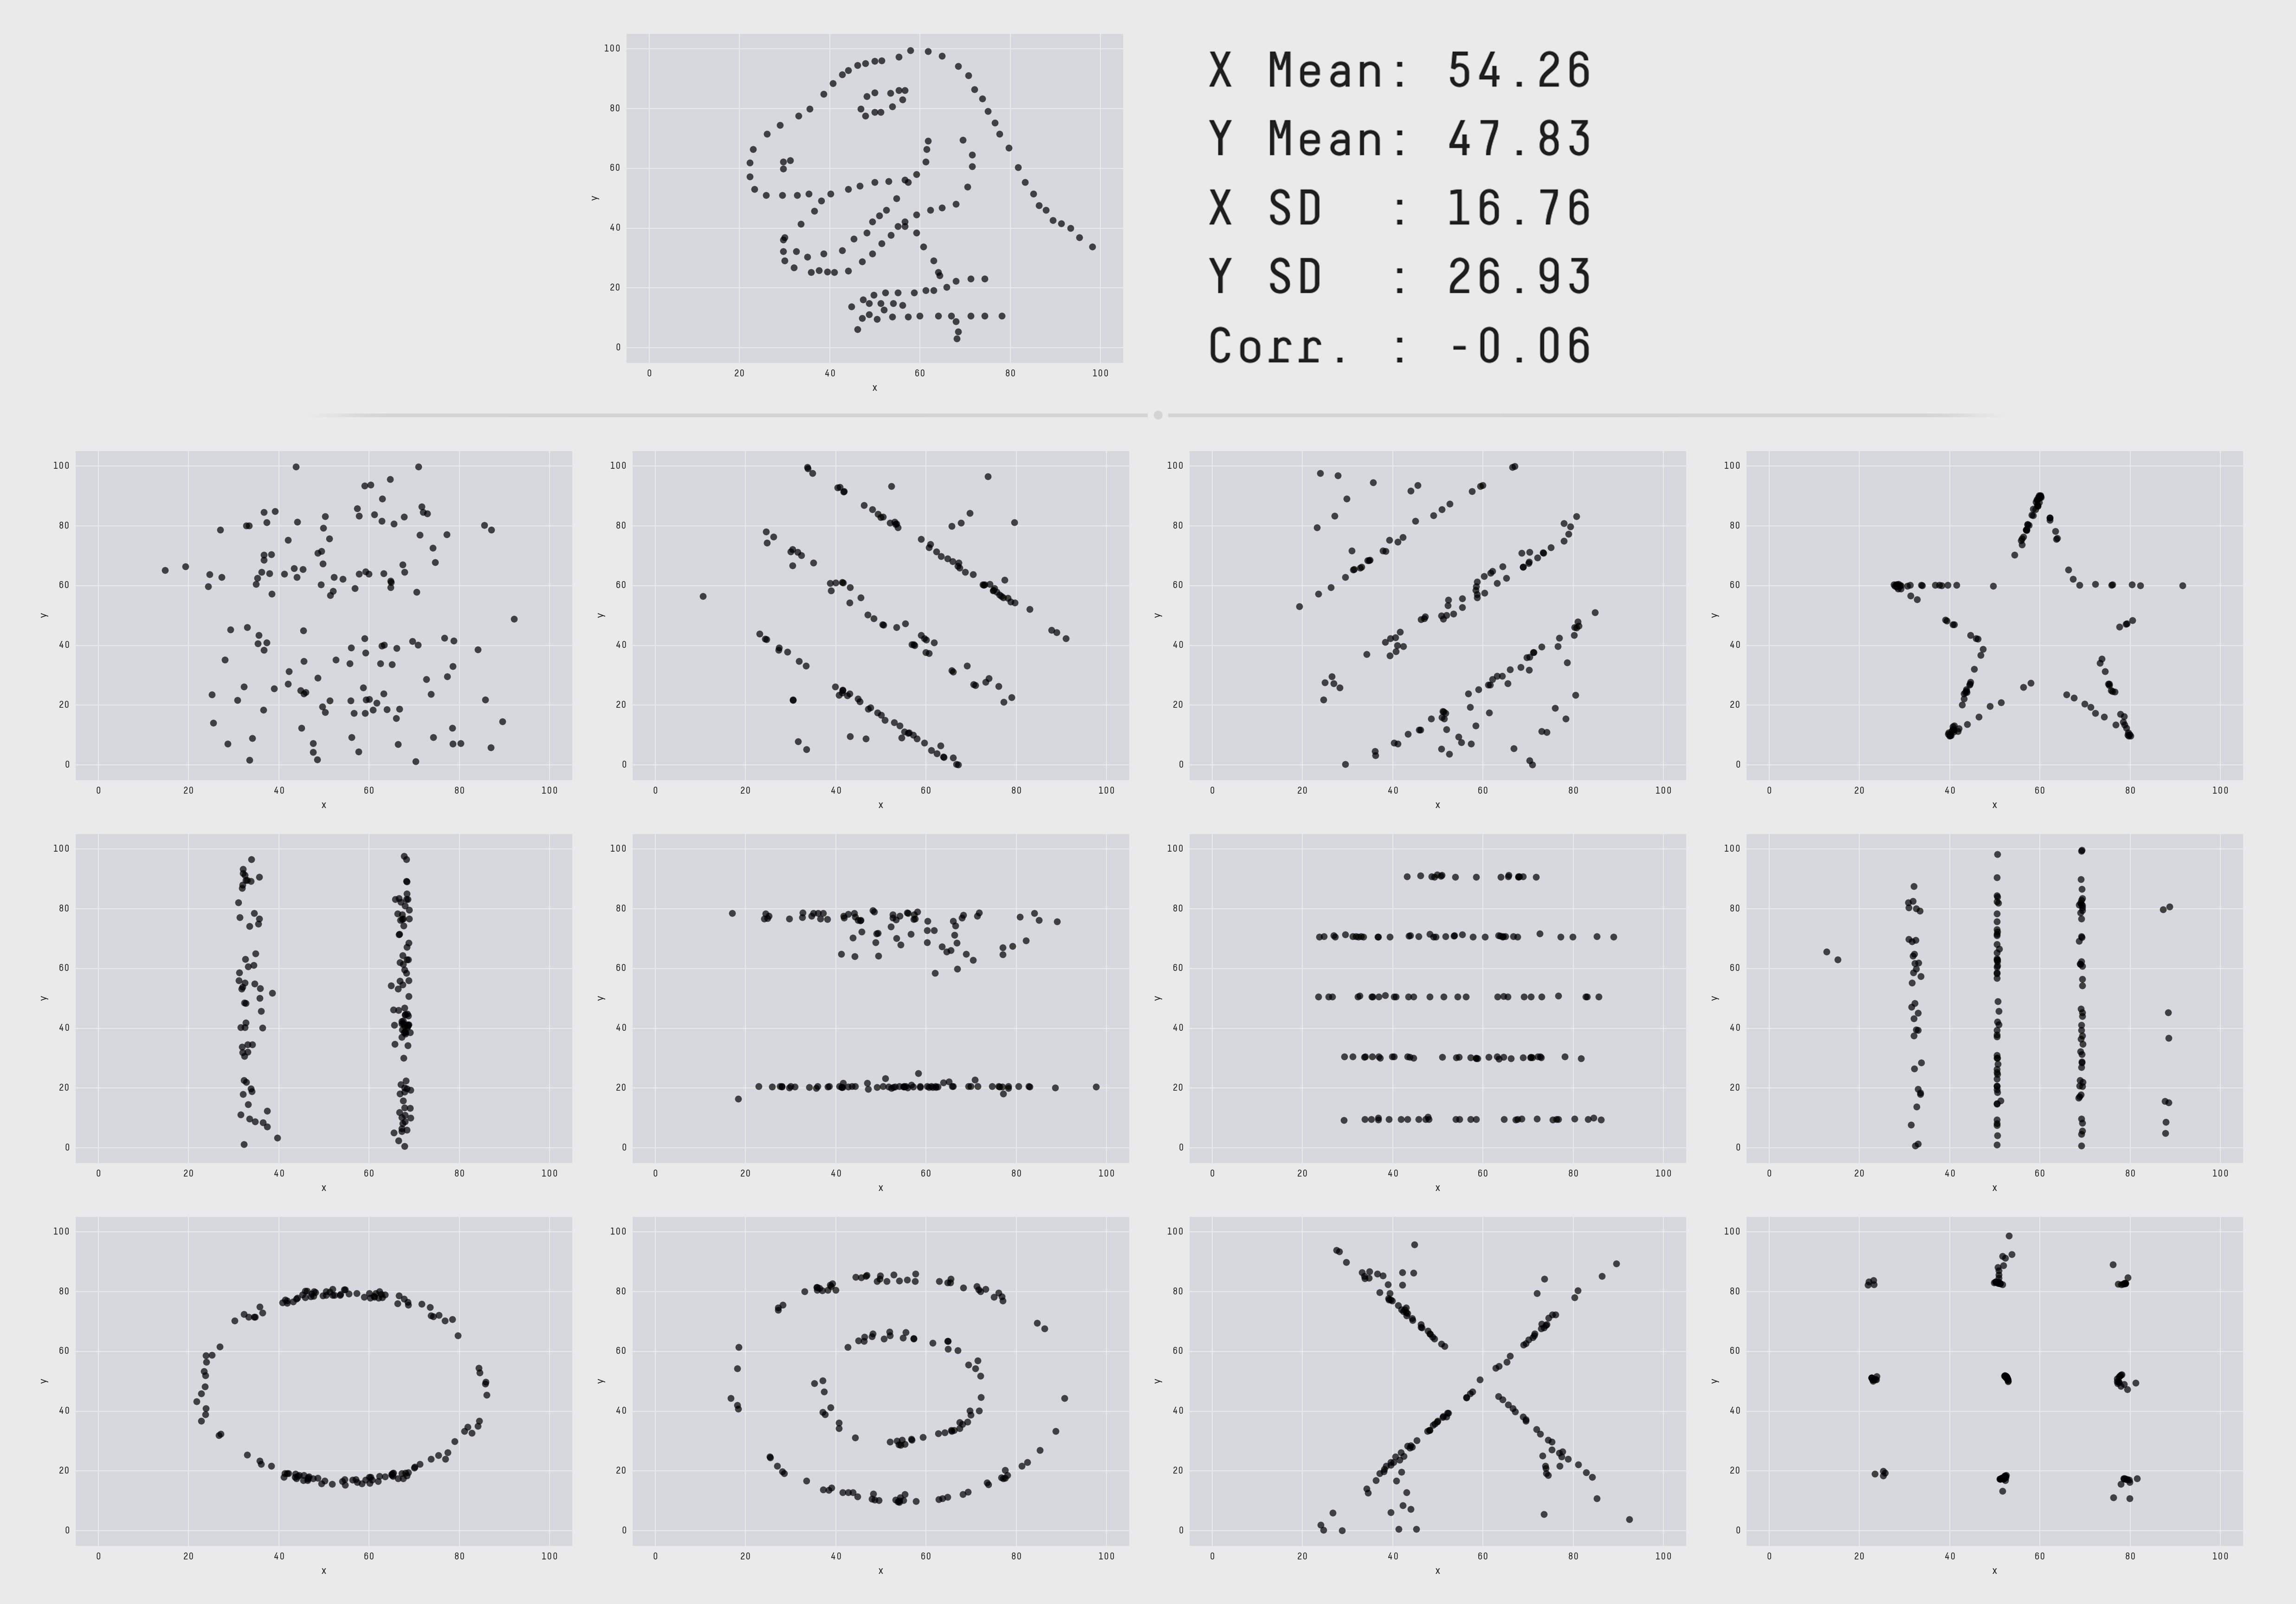
\includegraphics{datasaurus_alberto_cairo.png}
\caption{}
\end{figure}

This is why it's important to be aware of the underlying distribution of
data, and to not simply rely on summary statistics. Bar plots only show
summary statistics, and can thus hide potentially important differences
between groups.

    \subsubsection{Box plot}\label{box-plot}

One type of plot that \emph{does} reflect properties of distributions is
the box plot, also known as "box-and-whiskers plot". It quite literally
is two stacked boxes with whiskers on either side. Each element of the
plot represents a quartile (25\% of the observations) of the data. This
type of plot tells you about each group's median (the 50th percentile
lies between the second and third quartile), and gives you a rough idea
of what the distribution looks like. Some boxplots also include
'fliers': Values that lie outside the typical range, and could be
outliers.

Let's draw box plots for our two groups:

    \begin{Verbatim}[commandchars=\\\{\}]
{\color{incolor}In [{\color{incolor}11}]:} \PY{c+c1}{\PYZsh{} Draw a box for values from group x and group y. You can pass both }
         \PY{c+c1}{\PYZsh{} variables at the same time by combining them into a list, i.e. as}
         \PY{c+c1}{\PYZsh{} [x,y]. The same is true for the labels you would like to associate}
         \PY{c+c1}{\PYZsh{} with the groups.}
         \PY{n}{pyplot}\PY{o}{.}\PY{n}{boxplot}\PY{p}{(}\PY{p}{[}\PY{n}{x}\PY{p}{,}\PY{n}{y}\PY{p}{]}\PY{p}{,} \PY{n}{labels}\PY{o}{=}\PY{p}{[}\PY{l+s+s2}{\PYZdq{}}\PY{l+s+s2}{Group X}\PY{l+s+s2}{\PYZdq{}}\PY{p}{,}\PY{l+s+s2}{\PYZdq{}}\PY{l+s+s2}{Group Y}\PY{l+s+s2}{\PYZdq{}}\PY{p}{]}\PY{p}{)}
\end{Verbatim}


\begin{Verbatim}[commandchars=\\\{\}]
{\color{outcolor}Out[{\color{outcolor}11}]:} \{'boxes': [<matplotlib.lines.Line2D at 0x7fe9e118f1d0>,
           <matplotlib.lines.Line2D at 0x7fe9e119bb50>],
          'caps': [<matplotlib.lines.Line2D at 0x7fe9e118fb50>,
           <matplotlib.lines.Line2D at 0x7fe9e118ff50>,
           <matplotlib.lines.Line2D at 0x7fe9e11a57d0>,
           <matplotlib.lines.Line2D at 0x7fe9e11a5bd0>],
          'fliers': [<matplotlib.lines.Line2D at 0x7fe9e119b790>,
           <matplotlib.lines.Line2D at 0x7fe9e11b0410>],
          'means': [],
          'medians': [<matplotlib.lines.Line2D at 0x7fe9e119b390>,
           <matplotlib.lines.Line2D at 0x7fe9e11a5fd0>],
          'whiskers': [<matplotlib.lines.Line2D at 0x7fe9e118f290>,
           <matplotlib.lines.Line2D at 0x7fe9e118f750>,
           <matplotlib.lines.Line2D at 0x7fe9e119bf90>,
           <matplotlib.lines.Line2D at 0x7fe9e11a53d0>]\}
\end{Verbatim}
            
    \begin{center}
    \adjustimage{max size={0.9\linewidth}{0.9\paperheight}}{output_27_1.png}
    \end{center}
    { \hspace*{\fill} \\}
    
    This is a pretty good visualisation of the two groups. We can see their
central tendency, because the median is represented by the coloured
horizontal line. In addition, we can see how observations are spread
out. For group \texttt{x}, all quartiles are roughly equally big, which
demonstrates that the data is uniformly distributed. For group
\texttt{y}, we can see that the second and third quartile (the boxes)
are smaller than the first and fourth quartile (the whiskers). This
illustrates that the distribution is denser around the median.

What we still can't see from the current plot is what the shape of the
distribution is. For example, it seems like group \texttt{y} is a normal
distribution, but it could also be that all values within the second and
third quartile are the same. For example, they could all be -0.5 and
0.5, and it would result in the same box plot.

    \subsubsection{Violin plot}\label{violin-plot}

Where box plots do not typically reveal the exact shape of a
distribution, violin plots are designed to do exactly that. They apply a
\emph{kernel density estimate} to characterise the shape of a
distribution, and plot that instead of boxes and whiskers. Fliers are
still denoted with a different marker (although what is considered a
"flier" can differ between box plots and violin plots, or more
accurately, per what standards are set within the function to draw the
plots).

Let's see what a violin plot of our two groups would look like:

    \begin{Verbatim}[commandchars=\\\{\}]
{\color{incolor}In [{\color{incolor}12}]:} \PY{c+c1}{\PYZsh{} Draw a violin plot for values from group x and group y. As }
         \PY{c+c1}{\PYZsh{} with the box plot, you can pass both variables at the same}
         \PY{c+c1}{\PYZsh{} time by combining them into a list, i.e. as [x,y].}
         \PY{n}{pyplot}\PY{o}{.}\PY{n}{violinplot}\PY{p}{(}\PY{p}{[}\PY{n}{x}\PY{p}{,}\PY{n}{y}\PY{p}{]}\PY{p}{,} \PY{n}{showmeans}\PY{o}{=}\PY{n+nb+bp}{True}\PY{p}{)}
\end{Verbatim}


\begin{Verbatim}[commandchars=\\\{\}]
{\color{outcolor}Out[{\color{outcolor}12}]:} \{u'bodies': [<matplotlib.collections.PolyCollection at 0x7fe9e1116f90>,
           <matplotlib.collections.PolyCollection at 0x7fe9e11242d0>],
          u'cbars': <matplotlib.collections.LineCollection at 0x7fe9e1124f10>,
          u'cmaxes': <matplotlib.collections.LineCollection at 0x7fe9e1124890>,
          u'cmeans': <matplotlib.collections.LineCollection at 0x7fea0c438310>,
          u'cmins': <matplotlib.collections.LineCollection at 0x7fe9e1124bd0>\}
\end{Verbatim}
            
    \begin{center}
    \adjustimage{max size={0.9\linewidth}{0.9\paperheight}}{output_30_1.png}
    \end{center}
    { \hspace*{\fill} \\}
    
    The violin plot gives a much clearer picture of the actual distribution
of your data.

    \subsection{Choosing a visualisation
type}\label{choosing-a-visualisation-type}

As you have seen, different types of data visualisations exist, and each
come with their own benefits and downsides. Bar plots can be easily
understood, but also give you very little information about what
underlying data look like. In addition, whether or not it makes sense to
draw a bar highly depends on what kind of data you're visualising.
Adding error bars to bar plots to indicate the standard error of the
mean tells you something about the sampling process, whereas adding
error bars to indicate the standard deviation tells you something about
the sample.

If you're interested in visualising distributions in a more detailed
way, you could turn to box or violin plots. These provide a clearer
picture of what your data look like, and are still quite easy to
interpret.

What the best type of plot is depends on the data, and on what message
you would like your graph to illustrate. If you're simply saying "these
groups have different means", a bar plot with error bars that indicate
the standard error of the mean could work very well. However, if you're
trying to illustrate that two groups are from distributions with
different properties, you might need to turn to box or violin plots.

Finally, you can combine plots and types of visualisations. For example,
you could simply throw everything into one combined plot:

    \begin{Verbatim}[commandchars=\\\{\}]
{\color{incolor}In [{\color{incolor}13}]:} \PY{c+c1}{\PYZsh{} Determine the positions of the two groups\PYZsq{} visualisations}
         \PY{c+c1}{\PYZsh{} on the x\PYZhy{}axis.}
         \PY{n}{pos} \PY{o}{=} \PY{p}{[}\PY{l+m+mf}{0.5}\PY{p}{,} \PY{l+m+mf}{1.5}\PY{p}{]}
         
         \PY{c+c1}{\PYZsh{} Draw violin plots for each group, but don\PYZsq{}t draw the mean,}
         \PY{c+c1}{\PYZsh{} median, or extrema.}
         \PY{n}{vplot} \PY{o}{=} \PY{n}{pyplot}\PY{o}{.}\PY{n}{violinplot}\PY{p}{(}\PY{p}{[}\PY{n}{x}\PY{p}{,}\PY{n}{y}\PY{p}{]}\PY{p}{,} \PY{n}{positions}\PY{o}{=}\PY{n}{pos}\PY{p}{,} \PYZbs{}
             \PY{n}{showmeans}\PY{o}{=}\PY{n+nb+bp}{False}\PY{p}{,} \PY{n}{showmedians}\PY{o}{=}\PY{n+nb+bp}{False}\PY{p}{,} \PY{n}{showextrema}\PY{o}{=}\PY{n+nb+bp}{False}\PY{p}{)}
         \PY{c+c1}{\PYZsh{} Set the colour of the violin plot.}
         \PY{k}{for} \PY{n}{violin} \PY{o+ow}{in} \PY{n}{vplot}\PY{p}{[}\PY{l+s+s2}{\PYZdq{}}\PY{l+s+s2}{bodies}\PY{l+s+s2}{\PYZdq{}}\PY{p}{]}\PY{p}{:}
             \PY{n}{violin}\PY{o}{.}\PY{n}{set\PYZus{}color}\PY{p}{(}\PY{l+s+s2}{\PYZdq{}}\PY{l+s+s2}{\PYZsh{}FF69B4}\PY{l+s+s2}{\PYZdq{}}\PY{p}{)}
         \PY{c+c1}{\PYZsh{} Draw box plots for each groups on the same positions.}
         \PY{n}{bplot} \PY{o}{=} \PY{n}{pyplot}\PY{o}{.}\PY{n}{boxplot}\PY{p}{(}\PY{p}{[}\PY{n}{x}\PY{p}{,}\PY{n}{y}\PY{p}{]}\PY{p}{,} \PY{n}{positions}\PY{o}{=}\PY{n}{pos}\PY{p}{,} \PYZbs{}
             \PY{n}{labels}\PY{o}{=}\PY{p}{[}\PY{l+s+s2}{\PYZdq{}}\PY{l+s+s2}{Group X}\PY{l+s+s2}{\PYZdq{}}\PY{p}{,} \PY{l+s+s2}{\PYZdq{}}\PY{l+s+s2}{Group Y}\PY{l+s+s2}{\PYZdq{}}\PY{p}{]}\PY{p}{)}
         \PY{c+c1}{\PYZsh{} Set the colour of horizontal lines that indicate the median}
         \PY{c+c1}{\PYZsh{} in each box plot.}
         \PY{k}{for} \PY{n}{line} \PY{o+ow}{in} \PY{n}{bplot}\PY{p}{[}\PY{l+s+s2}{\PYZdq{}}\PY{l+s+s2}{medians}\PY{l+s+s2}{\PYZdq{}}\PY{p}{]}\PY{p}{:}
             \PY{n}{line}\PY{o}{.}\PY{n}{set\PYZus{}color}\PY{p}{(}\PY{l+s+s2}{\PYZdq{}}\PY{l+s+s2}{\PYZsh{}FF69B4}\PY{l+s+s2}{\PYZdq{}}\PY{p}{)}
         
         \PY{c+c1}{\PYZsh{} Finally, draw the individual data points for each group. The}
         \PY{c+c1}{\PYZsh{} points need to be plotted to the right of each of the }
         \PY{c+c1}{\PYZsh{} box/violin plots. To do so, we first need to create two }
         \PY{c+c1}{\PYZsh{} vectors that code for the position of each sample from each }
         \PY{c+c1}{\PYZsh{} group on the x\PYZhy{}axis.}
         \PY{n}{x\PYZus{}pos} \PY{o}{=} \PY{n}{numpy}\PY{o}{.}\PY{n}{ones}\PY{p}{(}\PY{n}{x}\PY{o}{.}\PY{n}{shape}\PY{p}{)} \PY{o}{*} \PY{n}{pos}\PY{p}{[}\PY{l+m+mi}{0}\PY{p}{]} \PY{o}{+} \PY{l+m+mf}{0.3}
         \PY{n}{y\PYZus{}pos} \PY{o}{=} \PY{n}{numpy}\PY{o}{.}\PY{n}{ones}\PY{p}{(}\PY{n}{y}\PY{o}{.}\PY{n}{shape}\PY{p}{)} \PY{o}{*} \PY{n}{pos}\PY{p}{[}\PY{l+m+mi}{1}\PY{p}{]} \PY{o}{+} \PY{l+m+mf}{0.3}
         \PY{c+c1}{\PYZsh{} Then, we simply need to plot the samples. The alpha keyword}
         \PY{c+c1}{\PYZsh{} indicates the transparancy of each sample.}
         \PY{n}{pyplot}\PY{o}{.}\PY{n}{plot}\PY{p}{(}\PY{n}{x\PYZus{}pos}\PY{p}{,} \PY{n}{x}\PY{p}{,} \PY{l+s+s1}{\PYZsq{}}\PY{l+s+s1}{.}\PY{l+s+s1}{\PYZsq{}}\PY{p}{,} \PY{n}{color}\PY{o}{=}\PY{l+s+s2}{\PYZdq{}}\PY{l+s+s2}{\PYZsh{}FF69B4}\PY{l+s+s2}{\PYZdq{}}\PY{p}{,} \PY{n}{alpha}\PY{o}{=}\PY{l+m+mf}{0.1}\PY{p}{)}
         \PY{n}{pyplot}\PY{o}{.}\PY{n}{plot}\PY{p}{(}\PY{n}{y\PYZus{}pos}\PY{p}{,} \PY{n}{y}\PY{p}{,} \PY{l+s+s1}{\PYZsq{}}\PY{l+s+s1}{.}\PY{l+s+s1}{\PYZsq{}}\PY{p}{,} \PY{n}{color}\PY{o}{=}\PY{l+s+s2}{\PYZdq{}}\PY{l+s+s2}{\PYZsh{}FF69B4}\PY{l+s+s2}{\PYZdq{}}\PY{p}{,} \PY{n}{alpha}\PY{o}{=}\PY{l+m+mf}{0.1}\PY{p}{)}
\end{Verbatim}


\begin{Verbatim}[commandchars=\\\{\}]
{\color{outcolor}Out[{\color{outcolor}13}]:} [<matplotlib.lines.Line2D at 0x7fe9e10cfe50>]
\end{Verbatim}
            
    \begin{center}
    \adjustimage{max size={0.9\linewidth}{0.9\paperheight}}{output_33_1.png}
    \end{center}
    { \hspace*{\fill} \\}
    
    

    \section{Statistics for group
comparisons}\label{statistics-for-group-comparisons}

In this next bit, we will be thinking about surprising events and group
differences. For example, if you read "men are taller than women", what
does that mean? Are all men taller than all women? Are most men taller
than most women? Or maybe men are taller than women \emph{on average}?
But what is a meaningful difference? Would it be meaningful if men, on
average, are 1 cm taller than women? Where do you draw the line? Also,
how many men and women would you need to test before you believe they
might have different average heights?

How we think about these questions has shaped our usage of statistics,
and you could even argue that how we use statistics has shaped how we
think about differences between groups. (That sounds a bit esoteric now,
but will become clearer towards the end of this section.)

    \subsection{Do you need to measure the entire
population?}\label{do-you-need-to-measure-the-entire-population}

Let's start with an example. When I'm in a debate with someone, but find
that I struggle to come up with a sensible argument, I like to hold my
breath in anger. My opponent is now left with only two options: Concede
the point, or engage in an impromptu breath-holding competition.
Obviously, this strategy only works if there is a high likelihood that I
can hold my breath longer than my opponent. How could we come to know
this likelihood?

First, we need to know how long I can hold my breath. This is easy: I
just hold my breath for as long as I can, and record how long it was
using a stopwatch. Let's say this was 83 seconds.

Next, we need to compare my breath-holding ability with the people I
usually debate. In order to do this, we need to establish who this
population is. As I work and live in Cambridge, the people I debate are
likely those who live here, and specifically those found in and around
the University. This is a problem: It's cumbersome and potentially
expensive to test \emph{everyone} who is associated with the University
of Cambridge.

Instead of the whole target population, maybe we could take a random
selection of people from them? If those people are representative, we
could use them to infer what the population must look like. This is
called a *sample".

In this case, I measured a convenience sample of my Cambridge
undergraduate students by by instructing them to hold their breath as
long as they could, and write down their time.

\emph{Of course, this is not ideal: Undergraduate students are around
the same age, and were made to do this as a stupid exercise in what
should have been a serious stats class. So perhaps the sample is biased,
and the measurement sub-optimal. Let's forget about those very
reasonable objections for now, and simply assume the sample is
representative of the wider Cambridge population. Or that I only ever
debate undergrads, as I'm not brave enough to take on anyone with higher
educational credentials than that.}

    \begin{Verbatim}[commandchars=\\\{\}]
{\color{incolor}In [{\color{incolor}14}]:} \PY{k+kn}{import} \PY{n+nn}{numpy}
         \PY{k+kn}{from} \PY{n+nn}{matplotlib} \PY{k+kn}{import} \PY{n}{pyplot}
         
         \PY{c+c1}{\PYZsh{} These times were measured during three stats classes.}
         \PY{c+c1}{\PYZsh{} Each class is in a different list.}
         \PY{n}{times\PYZus{}a} \PY{o}{=} \PY{p}{[}\PY{l+m+mf}{45.53}\PY{p}{,} \PY{l+m+mf}{41.30}\PY{p}{,} \PY{l+m+mf}{36.21}\PY{p}{,} \PY{l+m+mf}{49.3}\PY{p}{,} \PY{l+m+mf}{41.0}\PY{p}{,} \PY{l+m+mi}{63}\PY{p}{,} \PY{l+m+mf}{38.15}\PY{p}{,} \PYZbs{}
             \PY{l+m+mf}{35.1}\PY{p}{,} \PY{l+m+mf}{38.1}\PY{p}{,} \PY{l+m+mf}{47.9}\PY{p}{,} \PY{l+m+mf}{46.6}\PY{p}{,} \PY{l+m+mf}{23.0}\PY{p}{,} \PY{l+m+mf}{60.0}\PY{p}{,} \PY{l+m+mf}{42.0}\PY{p}{,} \PY{l+m+mf}{35.7}\PY{p}{,} \PY{l+m+mf}{41.2}\PY{p}{]}
         \PY{n}{times\PYZus{}b} \PY{o}{=} \PY{p}{[}\PY{l+m+mf}{42.0}\PY{p}{,} \PY{l+m+mf}{38.0}\PY{p}{,} \PY{l+m+mf}{46.0}\PY{p}{,} \PY{l+m+mf}{88.1}\PY{p}{,} \PY{l+m+mi}{125}\PY{p}{,} \PY{l+m+mf}{41.3}\PY{p}{,} \PY{l+m+mf}{36.0}\PY{p}{,} \PYZbs{}
             \PY{l+m+mf}{40.0}\PY{p}{,} \PY{l+m+mf}{43.7}\PY{p}{,} \PY{l+m+mf}{34.7}\PY{p}{,} \PY{l+m+mf}{38.4}\PY{p}{,} \PY{l+m+mf}{42.0}\PY{p}{,} \PY{l+m+mf}{61.0}\PY{p}{,} \PY{l+m+mf}{36.0}\PY{p}{,} \PY{l+m+mf}{43.4}\PY{p}{,} \PYZbs{}
             \PY{l+m+mf}{36.14}\PY{p}{,} \PY{l+m+mf}{18.23}\PY{p}{,} \PY{l+m+mf}{49.0}\PY{p}{,} \PY{l+m+mf}{38.0}\PY{p}{,} \PY{l+m+mf}{22.47}\PY{p}{,} \PY{l+m+mf}{35.51}\PY{p}{,} \PY{l+m+mf}{63.15}\PY{p}{,} \PYZbs{}
             \PY{l+m+mf}{35.2}\PY{p}{,} \PY{l+m+mf}{51.53}\PY{p}{,} \PY{l+m+mf}{34.13}\PY{p}{,} \PY{l+m+mf}{54.0}\PY{p}{,} \PY{l+m+mf}{43.2}\PY{p}{]}
         \PY{n}{times\PYZus{}c} \PY{o}{=} \PY{p}{[}\PY{l+m+mf}{94.0}\PY{p}{,} \PY{l+m+mf}{83.0}\PY{p}{,} \PY{l+m+mf}{95.0}\PY{p}{,} \PY{l+m+mf}{36.5}\PY{p}{,} \PY{l+m+mf}{49.0}\PY{p}{,} \PY{l+m+mf}{44.0}\PY{p}{,} \PY{l+m+mf}{43.0}\PY{p}{,} \PYZbs{}
             \PY{l+m+mf}{57.0}\PY{p}{,} \PY{l+m+mf}{35.8}\PY{p}{,} \PY{l+m+mf}{44.0}\PY{p}{,} \PY{l+m+mf}{44.4}\PY{p}{,} \PY{l+m+mf}{49.0}\PY{p}{,} \PY{l+m+mf}{39.0}\PY{p}{,} \PY{l+m+mf}{42.0}\PY{p}{,} \PY{l+m+mf}{35.0}\PY{p}{,} \PYZbs{}
             \PY{l+m+mf}{50.0}\PY{p}{,} \PY{l+m+mf}{53.0}\PY{p}{,} \PY{l+m+mf}{52.0}\PY{p}{,} \PY{l+m+mf}{33.0}\PY{p}{,} \PY{l+m+mf}{37.0}\PY{p}{,} \PY{l+m+mf}{48.0}\PY{p}{,} \PY{l+m+mf}{74.0}\PY{p}{,} \PY{l+m+mf}{41.0}\PY{p}{,} \PYZbs{}
             \PY{l+m+mf}{49.0}\PY{p}{,} \PY{l+m+mf}{38.0}\PY{p}{,} \PY{l+m+mf}{25.0}\PY{p}{,} \PY{l+m+mf}{61.0}\PY{p}{,} \PY{l+m+mf}{47.0}\PY{p}{,} \PY{l+m+mf}{41.0}\PY{p}{,} \PY{l+m+mf}{73.0}\PY{p}{]}
\end{Verbatim}


    The times were recorded in different lists. Fortunately, lists can
easily be combined together. You can simply use the \texttt{+} operator,
like so:

\texttt{times\ =\ times\_a\ +\ times\_b\ +\ times\_c}

However, you can also use the built-in \texttt{extend} method:

    \begin{Verbatim}[commandchars=\\\{\}]
{\color{incolor}In [{\color{incolor}15}]:} \PY{c+c1}{\PYZsh{} Let\PYZsq{}s add all the times together.}
         \PY{n}{times} \PY{o}{=} \PY{p}{[}\PY{p}{]}
         \PY{n}{times}\PY{o}{.}\PY{n}{extend}\PY{p}{(}\PY{n}{times\PYZus{}a}\PY{p}{)}
         \PY{n}{times}\PY{o}{.}\PY{n}{extend}\PY{p}{(}\PY{n}{times\PYZus{}b}\PY{p}{)}
         \PY{n}{times}\PY{o}{.}\PY{n}{extend}\PY{p}{(}\PY{n}{times\PYZus{}c}\PY{p}{)}
         
         \PY{c+c1}{\PYZsh{} Now that all the times are combined,}
         \PY{c+c1}{\PYZsh{} you can create a NumPy array from the}
         \PY{c+c1}{\PYZsh{} list of all times.}
         \PY{n}{t} \PY{o}{=} \PY{n}{numpy}\PY{o}{.}\PY{n}{array}\PY{p}{(}\PY{n}{times}\PY{p}{,} \PY{n}{dtype}\PY{o}{=}\PY{n+nb}{float}\PY{p}{)}
\end{Verbatim}


    Now that all the times are combined, and put into a single NumPy array,
you can create a histogram. You can use the same \texttt{histogram}
function from NumPy that was used in the examples above.

    \begin{Verbatim}[commandchars=\\\{\}]
{\color{incolor}In [{\color{incolor}16}]:} \PY{c+c1}{\PYZsh{} Make a histogram to count how frequently each breath\PYZhy{}}
         \PY{c+c1}{\PYZsh{} holding time occurs in the sample.}
         \PY{n}{hist}\PY{p}{,} \PY{n}{edges} \PY{o}{=} \PY{n}{numpy}\PY{o}{.}\PY{n}{histogram}\PY{p}{(}\PY{n}{t}\PY{p}{,} \PY{n}{bins}\PY{o}{=}\PY{l+m+mi}{20}\PY{p}{)}
         \PY{n}{bin\PYZus{}centres} \PY{o}{=} \PY{n}{edges}\PY{p}{[}\PY{p}{:}\PY{o}{\PYZhy{}}\PY{l+m+mi}{1}\PY{p}{]} \PY{o}{+} \PY{n}{numpy}\PY{o}{.}\PY{n}{diff}\PY{p}{(}\PY{n}{edges}\PY{p}{)}\PY{o}{/}\PY{l+m+mf}{2.0}
\end{Verbatim}


    Matplotlib's \texttt{plot} function can be used to draw lines. It needs
the x and y values, and you can also pass a line style. Here we pass
\texttt{-} to create a continuous line. Alternatives include
\texttt{-\/-} for a dashed line, \texttt{-.} for a dash-dot line, and
\texttt{:} for a dotted line. You can also pass \texttt{o} for round
markers without a line, or \texttt{s} for square markers without a line.
Finally, you can combine line and marker characters, for example
\texttt{-o} for a continuous line with round markers.

The \texttt{lw} keyword argument sets the \textbf{l}ine \textbf{w}idth,
and the \texttt{color} argument the colour. Here we pass the hex value
for hot pink, but you can also pass colour names, or even (r,g,b) values
(with numbers for each of the red, green, and blue values between 0 and
1)).

    \begin{Verbatim}[commandchars=\\\{\}]
{\color{incolor}In [{\color{incolor}17}]:} \PY{c+c1}{\PYZsh{} Plot the histogram.}
         \PY{n}{pyplot}\PY{o}{.}\PY{n}{plot}\PY{p}{(}\PY{n}{bin\PYZus{}centres}\PY{p}{,} \PY{n}{hist}\PY{p}{,} \PY{l+s+s1}{\PYZsq{}}\PY{l+s+s1}{\PYZhy{}}\PY{l+s+s1}{\PYZsq{}}\PY{p}{,} \PY{n}{lw}\PY{o}{=}\PY{l+m+mi}{3}\PY{p}{,} \PY{n}{color}\PY{o}{=}\PY{l+s+s2}{\PYZdq{}}\PY{l+s+s2}{\PYZsh{}FF69B4}\PY{l+s+s2}{\PYZdq{}}\PY{p}{)}
         \PY{n}{pyplot}\PY{o}{.}\PY{n}{ylabel}\PY{p}{(}\PY{l+s+s2}{\PYZdq{}}\PY{l+s+s2}{Number of observations}\PY{l+s+s2}{\PYZdq{}}\PY{p}{,} \PY{n}{fontsize}\PY{o}{=}\PY{l+m+mi}{16}\PY{p}{)}
         \PY{n}{pyplot}\PY{o}{.}\PY{n}{xlabel}\PY{p}{(}\PY{l+s+s2}{\PYZdq{}}\PY{l+s+s2}{Hold\PYZhy{}your\PYZhy{}breath times (sec)}\PY{l+s+s2}{\PYZdq{}}\PY{p}{,} \PY{n}{fontsize}\PY{o}{=}\PY{l+m+mi}{16}\PY{p}{)}
         \PY{n}{pyplot}\PY{o}{.}\PY{n}{show}\PY{p}{(}\PY{p}{)}
\end{Verbatim}


    \begin{center}
    \adjustimage{max size={0.9\linewidth}{0.9\paperheight}}{output_43_0.png}
    \end{center}
    { \hspace*{\fill} \\}
    
    Great, now we know what the population should roughly look like. From
the histogram, we can read that the most likely breath-holding times are
around 40 seconds. We can also see that the times are quite variable:
They range all the way from 20 to 120 seconds! Even if we look at just
the times with the most observations, there's a substantial range from
about 30-50 seconds.

    \subsection{When is a value noticably
different?}\label{when-is-a-value-noticably-different}

So what about my 83 seconds? Is it a surprising value within this
population? More importantly, does it make me likely to win
debate-avoiding breath-holding competitions? One way to compute this, is
by calculating how many people can hold their breath for less long than
me. This proportion would reflect the probability of encountering
someone who can hold their breath for less long, and thus of my winning.

    \begin{Verbatim}[commandchars=\\\{\}]
{\color{incolor}In [{\color{incolor}18}]:} \PY{c+c1}{\PYZsh{} Define my value.}
         \PY{n}{v} \PY{o}{=} \PY{l+m+mf}{83.0}
         
         \PY{c+c1}{\PYZsh{} Plot the histogram.}
         \PY{n}{pyplot}\PY{o}{.}\PY{n}{plot}\PY{p}{(}\PY{n}{bin\PYZus{}centres}\PY{p}{,} \PY{n}{hist}\PY{p}{,} \PY{l+s+s1}{\PYZsq{}}\PY{l+s+s1}{\PYZhy{}}\PY{l+s+s1}{\PYZsq{}}\PY{p}{,} \PY{n}{lw}\PY{o}{=}\PY{l+m+mi}{3}\PY{p}{,} \PY{n}{color}\PY{o}{=}\PY{l+s+s2}{\PYZdq{}}\PY{l+s+s2}{\PYZsh{}FF69B4}\PY{l+s+s2}{\PYZdq{}}\PY{p}{)}
         \PY{n}{pyplot}\PY{o}{.}\PY{n}{ylabel}\PY{p}{(}\PY{l+s+s2}{\PYZdq{}}\PY{l+s+s2}{Number of observations}\PY{l+s+s2}{\PYZdq{}}\PY{p}{,} \PY{n}{fontsize}\PY{o}{=}\PY{l+m+mi}{16}\PY{p}{)}
         \PY{n}{pyplot}\PY{o}{.}\PY{n}{xlabel}\PY{p}{(}\PY{l+s+s2}{\PYZdq{}}\PY{l+s+s2}{Hold\PYZhy{}your\PYZhy{}breath times (sec)}\PY{l+s+s2}{\PYZdq{}}\PY{p}{,} \PY{n}{fontsize}\PY{o}{=}\PY{l+m+mi}{16}\PY{p}{)}
         
         \PY{c+c1}{\PYZsh{} Plot my value in there.}
         \PY{n}{pyplot}\PY{o}{.}\PY{n}{axvline}\PY{p}{(}\PY{n}{v}\PY{p}{,} \PY{n}{linestyle}\PY{o}{=}\PY{l+s+s2}{\PYZdq{}}\PY{l+s+s2}{\PYZhy{}\PYZhy{}}\PY{l+s+s2}{\PYZdq{}}\PY{p}{,} \PY{n}{lw}\PY{o}{=}\PY{l+m+mi}{3}\PY{p}{,} \PY{n}{color}\PY{o}{=}\PY{l+s+s2}{\PYZdq{}}\PY{l+s+s2}{\PYZsh{}FF0000}\PY{l+s+s2}{\PYZdq{}}\PY{p}{)}
         \PY{n}{pyplot}\PY{o}{.}\PY{n}{show}\PY{p}{(}\PY{p}{)}
\end{Verbatim}


    \begin{center}
    \adjustimage{max size={0.9\linewidth}{0.9\paperheight}}{output_46_0.png}
    \end{center}
    { \hspace*{\fill} \\}
    
    The visualisation is nice, but we need to compute how many values in the
distribution were actually lower than our target value. To do so, we can
use the fact that Booleans can be read as 0s and 1s.

In order to know which values in \texttt{t} are lower than the target
value \texttt{v}, we can create a Boolean array by using
\texttt{t\ \textless{}\ v}. As you might recall from the previous
worksheet, this should result in an array with a True value for every
value in \texttt{t} that was lower than \texttt{v}, and False for every
value that was not.

Because True can be considered 1, and False 0, we can convert a Boolean
array to integer values. This can be done using the \texttt{astype}
function that is built into NumPy arrays. This returns an array with 1
instead of True, and 0 instead of False. The sum of this array is the
number of times the original was True. (In this case that is the number
of values in \texttt{t} that is lower than \texttt{v}!)

    \begin{Verbatim}[commandchars=\\\{\}]
{\color{incolor}In [{\color{incolor}19}]:} \PY{c+c1}{\PYZsh{} Compute how many values were lower.}
         \PY{n}{lower} \PY{o}{=} \PY{n}{t} \PY{o}{\PYZlt{}} \PY{n}{v}
         \PY{n}{n\PYZus{}lower} \PY{o}{=} \PY{n}{numpy}\PY{o}{.}\PY{n}{sum}\PY{p}{(}\PY{n}{lower}\PY{o}{.}\PY{n}{astype}\PY{p}{(}\PY{n+nb}{int}\PY{p}{)}\PY{p}{)}
         \PY{n}{p\PYZus{}lower} \PY{o}{=} \PY{n+nb}{float}\PY{p}{(}\PY{n}{n\PYZus{}lower}\PY{p}{)} \PY{o}{/} \PY{n+nb}{len}\PY{p}{(}\PY{n}{t}\PY{p}{)}
         
         \PY{k}{print}\PY{p}{(}\PY{l+s+s2}{\PYZdq{}}\PY{l+s+s2}{\PYZob{}\PYZcb{}/\PYZob{}\PYZcb{} observations (prop=\PYZob{}\PYZcb{}) lower than \PYZob{}\PYZcb{} seconds}\PY{l+s+s2}{\PYZdq{}}\PY{o}{.}\PY{n}{format}\PY{p}{(} \PYZbs{}
             \PY{n}{n\PYZus{}lower}\PY{p}{,} \PY{n+nb}{len}\PY{p}{(}\PY{n}{t}\PY{p}{)}\PY{p}{,} \PY{n+nb}{round}\PY{p}{(}\PY{n}{p\PYZus{}lower}\PY{p}{,} \PY{n}{ndigits}\PY{o}{=}\PY{l+m+mi}{2}\PY{p}{)}\PY{p}{,} \PY{n+nb}{round}\PY{p}{(}\PY{n}{v}\PY{p}{,} \PY{n}{ndigits}\PY{o}{=}\PY{l+m+mi}{1}\PY{p}{)}\PY{p}{)}\PY{p}{)}
\end{Verbatim}


    \begin{Verbatim}[commandchars=\\\{\}]
68/73 observations (prop=0.93) lower than 83.0 seconds

    \end{Verbatim}

    As you can see, about 93\% of our sample falls below my time. This means
that I would lose my argument only in 7\% of cases.

Another way of thinking about this is to ask whether my time is
surprising given the population. You could argue that my breath-holding
ability is somewhat rare, with only 7\% of people doing better. You
could also argue that it's within the normal population, and that there
are quite a lot of people who can hold their breath for much longer.
Where you draw this line of what is surprising is arbitrary, and depends
on context.

What you just calculated is akin to a \emph{p value}. Our measured data
forms a \emph{probability distribution} that tells you just how likely
each breath-holding time is. When a time is associated with value of
p=0.07, it tells you that 93\% of a population is expected to score
lower.

If you would like to play around with distributions and p values some
more, this Shiny app is great: https://gallery.shinyapps.io/dist\_calc/

    \subsection{When is a whole group of values noticably different from
what I
expected?}\label{when-is-a-whole-group-of-values-noticably-different-from-what-i-expected}

Imagine that you are an alien, unfamiliar with the human race. You came
upon Earth, found a funny-looking mammal, and decided to bring it back
to your ship. Unfortunately, you notice too late that humans don't
thrive in your water tank, but in fact drown. You grab another one, and
observe that they fare better in an environment closer to the earths
atmosphere. It turns out they have this weird thing where they suck in
air, and then breathe it out again. You assume that this is why they
didn't do well in your water tank.

You now wonder whether humans have to continuously do this breathing
thing, or whether they might have some internal reserves. From your
initial water tank mishap, you assume that humans simply cannot do
without continuosly inhaling and exhaling air. Hence, your hypothesis is
that humans cannot hold their breath. Well, maybe for like 30 seconds,
because that's how long your first human visibly struggled in the water
tank.

You decide to run a study\(^*\): You extract a number of Cambridge
undergraduates, ask your subjects to stop exhaling new air, and measure
how long it takes before they have to inhale again. Of course, you end
up with the same data as we've just seen.

\emph{* You don't have to get IRB approval, because it is known that
humans are primitive life that probably isn't even conscious. Many even
wonder whether they feel pain at all, and even if they do, they probably
wouldn't experience it in the same way as you, or even be able to
conciously remember it.}

    \begin{Verbatim}[commandchars=\\\{\}]
{\color{incolor}In [{\color{incolor}20}]:} \PY{k+kn}{import} \PY{n+nn}{numpy}
         \PY{k+kn}{from} \PY{n+nn}{matplotlib} \PY{k+kn}{import} \PY{n}{pyplot}
         
         \PY{c+c1}{\PYZsh{} These times were measured during three stats classes.}
         \PY{n}{times\PYZus{}a} \PY{o}{=} \PY{p}{[}\PY{l+m+mf}{45.53}\PY{p}{,} \PY{l+m+mf}{41.30}\PY{p}{,} \PY{l+m+mf}{36.21}\PY{p}{,} \PY{l+m+mf}{49.3}\PY{p}{,} \PY{l+m+mf}{41.0}\PY{p}{,} \PY{l+m+mi}{63}\PY{p}{,} \PY{l+m+mf}{38.15}\PY{p}{,} \PYZbs{}
             \PY{l+m+mf}{35.1}\PY{p}{,} \PY{l+m+mf}{38.1}\PY{p}{,} \PY{l+m+mf}{47.9}\PY{p}{,} \PY{l+m+mf}{46.6}\PY{p}{,} \PY{l+m+mf}{23.0}\PY{p}{,} \PY{l+m+mf}{60.0}\PY{p}{,} \PY{l+m+mf}{42.0}\PY{p}{,} \PY{l+m+mf}{35.7}\PY{p}{,} \PY{l+m+mf}{41.2}\PY{p}{]}
         \PY{n}{times\PYZus{}b} \PY{o}{=} \PY{p}{[}\PY{l+m+mf}{42.0}\PY{p}{,} \PY{l+m+mf}{38.0}\PY{p}{,} \PY{l+m+mf}{46.0}\PY{p}{,} \PY{l+m+mf}{88.1}\PY{p}{,} \PY{l+m+mi}{125}\PY{p}{,} \PY{l+m+mf}{41.3}\PY{p}{,} \PY{l+m+mf}{36.0}\PY{p}{,} \PYZbs{}
             \PY{l+m+mf}{40.0}\PY{p}{,} \PY{l+m+mf}{43.7}\PY{p}{,} \PY{l+m+mf}{34.7}\PY{p}{,} \PY{l+m+mf}{38.4}\PY{p}{,} \PY{l+m+mf}{42.0}\PY{p}{,} \PY{l+m+mf}{61.0}\PY{p}{,} \PY{l+m+mf}{36.0}\PY{p}{,} \PY{l+m+mf}{43.4}\PY{p}{,} \PYZbs{}
             \PY{l+m+mf}{36.14}\PY{p}{,} \PY{l+m+mf}{18.23}\PY{p}{,} \PY{l+m+mf}{49.0}\PY{p}{,} \PY{l+m+mf}{38.0}\PY{p}{,} \PY{l+m+mf}{22.47}\PY{p}{,} \PY{l+m+mf}{35.51}\PY{p}{,} \PY{l+m+mf}{63.15}\PY{p}{,} \PYZbs{}
             \PY{l+m+mf}{35.2}\PY{p}{,} \PY{l+m+mf}{51.53}\PY{p}{,} \PY{l+m+mf}{34.13}\PY{p}{,} \PY{l+m+mf}{54.0}\PY{p}{,} \PY{l+m+mf}{43.2}\PY{p}{]}
         \PY{n}{times\PYZus{}c} \PY{o}{=} \PY{p}{[}\PY{l+m+mf}{94.0}\PY{p}{,} \PY{l+m+mf}{83.0}\PY{p}{,} \PY{l+m+mf}{95.0}\PY{p}{,} \PY{l+m+mf}{36.5}\PY{p}{,} \PY{l+m+mf}{49.0}\PY{p}{,} \PY{l+m+mf}{44.0}\PY{p}{,} \PY{l+m+mf}{43.0}\PY{p}{,} \PYZbs{}
             \PY{l+m+mf}{57.0}\PY{p}{,} \PY{l+m+mf}{35.8}\PY{p}{,} \PY{l+m+mf}{44.0}\PY{p}{,} \PY{l+m+mf}{44.4}\PY{p}{,} \PY{l+m+mf}{49.0}\PY{p}{,} \PY{l+m+mf}{39.0}\PY{p}{,} \PY{l+m+mf}{42.0}\PY{p}{,} \PY{l+m+mf}{35.0}\PY{p}{,} \PYZbs{}
             \PY{l+m+mf}{50.0}\PY{p}{,} \PY{l+m+mf}{53.0}\PY{p}{,} \PY{l+m+mf}{52.0}\PY{p}{,} \PY{l+m+mf}{33.0}\PY{p}{,} \PY{l+m+mf}{37.0}\PY{p}{,} \PY{l+m+mf}{48.0}\PY{p}{,} \PY{l+m+mf}{74.0}\PY{p}{,} \PY{l+m+mf}{41.0}\PY{p}{,} \PYZbs{}
             \PY{l+m+mf}{49.0}\PY{p}{,} \PY{l+m+mf}{38.0}\PY{p}{,} \PY{l+m+mf}{25.0}\PY{p}{,} \PY{l+m+mf}{61.0}\PY{p}{,} \PY{l+m+mf}{47.0}\PY{p}{,} \PY{l+m+mf}{41.0}\PY{p}{,} \PY{l+m+mf}{73.0}\PY{p}{]}
         
         \PY{c+c1}{\PYZsh{} Let\PYZsq{}s add all the times together.}
         \PY{n}{times} \PY{o}{=} \PY{p}{[}\PY{p}{]}
         \PY{n}{times}\PY{o}{.}\PY{n}{extend}\PY{p}{(}\PY{n}{times\PYZus{}a}\PY{p}{)}
         \PY{n}{times}\PY{o}{.}\PY{n}{extend}\PY{p}{(}\PY{n}{times\PYZus{}b}\PY{p}{)}
         \PY{n}{times}\PY{o}{.}\PY{n}{extend}\PY{p}{(}\PY{n}{times\PYZus{}c}\PY{p}{)}
         \PY{n}{t} \PY{o}{=} \PY{n}{numpy}\PY{o}{.}\PY{n}{array}\PY{p}{(}\PY{n}{times}\PY{p}{,} \PY{n}{dtype}\PY{o}{=}\PY{n+nb}{float}\PY{p}{)}
         
         \PY{c+c1}{\PYZsh{} Make a histogram to count how frequently each breath\PYZhy{}}
         \PY{c+c1}{\PYZsh{} holding time occurs in the sample.}
         \PY{n}{hist}\PY{p}{,} \PY{n}{edges} \PY{o}{=} \PY{n}{numpy}\PY{o}{.}\PY{n}{histogram}\PY{p}{(}\PY{n}{t}\PY{p}{,} \PY{n}{bins}\PY{o}{=}\PY{l+m+mi}{20}\PY{p}{)}
         \PY{n}{bin\PYZus{}centres} \PY{o}{=} \PY{n}{edges}\PY{p}{[}\PY{p}{:}\PY{o}{\PYZhy{}}\PY{l+m+mi}{1}\PY{p}{]} \PY{o}{+} \PY{n}{numpy}\PY{o}{.}\PY{n}{diff}\PY{p}{(}\PY{n}{edges}\PY{p}{)}\PY{o}{/}\PY{l+m+mf}{2.0}
         
         \PY{c+c1}{\PYZsh{} Plot the histogram.}
         \PY{n}{pyplot}\PY{o}{.}\PY{n}{plot}\PY{p}{(}\PY{n}{bin\PYZus{}centres}\PY{p}{,} \PY{n}{hist}\PY{p}{,} \PY{l+s+s1}{\PYZsq{}}\PY{l+s+s1}{\PYZhy{}}\PY{l+s+s1}{\PYZsq{}}\PY{p}{,} \PY{n}{lw}\PY{o}{=}\PY{l+m+mi}{3}\PY{p}{,} \PY{n}{color}\PY{o}{=}\PY{l+s+s2}{\PYZdq{}}\PY{l+s+s2}{\PYZsh{}FF69B4}\PY{l+s+s2}{\PYZdq{}}\PY{p}{)}
         \PY{n}{pyplot}\PY{o}{.}\PY{n}{ylabel}\PY{p}{(}\PY{l+s+s2}{\PYZdq{}}\PY{l+s+s2}{Number of observations}\PY{l+s+s2}{\PYZdq{}}\PY{p}{,} \PY{n}{fontsize}\PY{o}{=}\PY{l+m+mi}{16}\PY{p}{)}
         \PY{n}{pyplot}\PY{o}{.}\PY{n}{xlabel}\PY{p}{(}\PY{l+s+s2}{\PYZdq{}}\PY{l+s+s2}{Hold\PYZhy{}your\PYZhy{}breath times (sec)}\PY{l+s+s2}{\PYZdq{}}\PY{p}{,} \PY{n}{fontsize}\PY{o}{=}\PY{l+m+mi}{16}\PY{p}{)}
         \PY{n}{pyplot}\PY{o}{.}\PY{n}{show}\PY{p}{(}\PY{p}{)}
\end{Verbatim}


    \begin{center}
    \adjustimage{max size={0.9\linewidth}{0.9\paperheight}}{output_51_0.png}
    \end{center}
    { \hspace*{\fill} \\}
    
    The above is the same code as before, just combined into a single
snippet for convenience. Your next question is simple: Is this
distribution what you expected? Do the results confirm your hypothesis
that humans cannot hold their breath?

Your expectation was that humans could not hold their breath, or more
specifically that they wouldn't be able to for more than about 30
seconds. The difficulty is in translating your expectation to the
language of numbers and distributions.

Essentially, what you're saying is that you expect the average human
being to be able to hold their breath for a maximum of 30 seconds. That
doesn't have to mean that all humans abide by that: some will be worse,
and some beter. In terms of a distribution, you're expecting that the
central tendency of the distribution is around 30 seconds.

Let's plot your expected average in the histogram, and see if it aligns
with the real average. We can do this with code that is very similar to
the code you used above.

    \begin{Verbatim}[commandchars=\\\{\}]
{\color{incolor}In [{\color{incolor}21}]:} \PY{c+c1}{\PYZsh{} Define expected average value.}
         \PY{n}{m\PYZus{}expected} \PY{o}{=} \PY{l+m+mi}{30}
         
         \PY{c+c1}{\PYZsh{} Compute the real average.}
         \PY{n}{m\PYZus{}real} \PY{o}{=} \PY{n}{numpy}\PY{o}{.}\PY{n}{mean}\PY{p}{(}\PY{n}{t}\PY{p}{)}
         \PY{k}{print}\PY{p}{(}\PY{l+s+s2}{\PYZdq{}}\PY{l+s+s2}{Expected mean: \PYZob{}\PYZcb{}, real mean: \PYZob{}\PYZcb{}}\PY{l+s+s2}{\PYZdq{}}\PY{o}{.}\PY{n}{format}\PY{p}{(} \PYZbs{}
             \PY{n+nb}{round}\PY{p}{(}\PY{n}{m\PYZus{}expected}\PY{p}{,} \PY{n}{ndigits}\PY{o}{=}\PY{l+m+mi}{2}\PY{p}{)}\PY{p}{,} \PY{n+nb}{round}\PY{p}{(}\PY{n}{m\PYZus{}real}\PY{p}{,} \PY{n}{ndigits}\PY{o}{=}\PY{l+m+mi}{2}\PY{p}{)}\PY{p}{)}\PY{p}{)}
         
         \PY{c+c1}{\PYZsh{} Plot the histogram.}
         \PY{n}{pyplot}\PY{o}{.}\PY{n}{plot}\PY{p}{(}\PY{n}{bin\PYZus{}centres}\PY{p}{,} \PY{n}{hist}\PY{p}{,} \PY{l+s+s1}{\PYZsq{}}\PY{l+s+s1}{\PYZhy{}}\PY{l+s+s1}{\PYZsq{}}\PY{p}{,} \PY{n}{lw}\PY{o}{=}\PY{l+m+mi}{3}\PY{p}{,} \PY{n}{color}\PY{o}{=}\PY{l+s+s2}{\PYZdq{}}\PY{l+s+s2}{\PYZsh{}FF69B4}\PY{l+s+s2}{\PYZdq{}}\PY{p}{)}
         \PY{n}{pyplot}\PY{o}{.}\PY{n}{ylabel}\PY{p}{(}\PY{l+s+s2}{\PYZdq{}}\PY{l+s+s2}{Number of observations}\PY{l+s+s2}{\PYZdq{}}\PY{p}{,} \PY{n}{fontsize}\PY{o}{=}\PY{l+m+mi}{16}\PY{p}{)}
         \PY{n}{pyplot}\PY{o}{.}\PY{n}{xlabel}\PY{p}{(}\PY{l+s+s2}{\PYZdq{}}\PY{l+s+s2}{Hold\PYZhy{}your\PYZhy{}breath times (sec)}\PY{l+s+s2}{\PYZdq{}}\PY{p}{,} \PY{n}{fontsize}\PY{o}{=}\PY{l+m+mi}{16}\PY{p}{)}
         
         \PY{c+c1}{\PYZsh{} Plot the expected and real averages in there.}
         \PY{n}{pyplot}\PY{o}{.}\PY{n}{axvline}\PY{p}{(}\PY{n}{m\PYZus{}expected}\PY{p}{,} \PY{n}{linestyle}\PY{o}{=}\PY{l+s+s2}{\PYZdq{}}\PY{l+s+s2}{\PYZhy{}\PYZhy{}}\PY{l+s+s2}{\PYZdq{}}\PY{p}{,} \PY{n}{lw}\PY{o}{=}\PY{l+m+mi}{3}\PY{p}{,} \PY{n}{color}\PY{o}{=}\PY{l+s+s2}{\PYZdq{}}\PY{l+s+s2}{\PYZsh{}FF0000}\PY{l+s+s2}{\PYZdq{}}\PY{p}{,} \PYZbs{}
             \PY{n}{label}\PY{o}{=}\PY{l+s+s2}{\PYZdq{}}\PY{l+s+s2}{hypothesis}\PY{l+s+s2}{\PYZdq{}}\PY{p}{)}
         \PY{n}{pyplot}\PY{o}{.}\PY{n}{axvline}\PY{p}{(}\PY{n}{m\PYZus{}real}\PY{p}{,} \PY{n}{linestyle}\PY{o}{=}\PY{l+s+s2}{\PYZdq{}}\PY{l+s+s2}{\PYZhy{}\PYZhy{}}\PY{l+s+s2}{\PYZdq{}}\PY{p}{,} \PY{n}{lw}\PY{o}{=}\PY{l+m+mi}{3}\PY{p}{,} \PY{n}{color}\PY{o}{=}\PY{l+s+s2}{\PYZdq{}}\PY{l+s+s2}{\PYZsh{}FF69B4}\PY{l+s+s2}{\PYZdq{}}\PY{p}{,} \PYZbs{}
             \PY{n}{label}\PY{o}{=}\PY{l+s+s2}{\PYZdq{}}\PY{l+s+s2}{data}\PY{l+s+s2}{\PYZdq{}}\PY{p}{)}
         \PY{n}{pyplot}\PY{o}{.}\PY{n}{legend}\PY{p}{(}\PY{n}{loc}\PY{o}{=}\PY{l+s+s2}{\PYZdq{}}\PY{l+s+s2}{upper right}\PY{l+s+s2}{\PYZdq{}}\PY{p}{)}
         \PY{n}{pyplot}\PY{o}{.}\PY{n}{show}\PY{p}{(}\PY{p}{)}
\end{Verbatim}


    \begin{Verbatim}[commandchars=\\\{\}]
Expected mean: 30.0, real mean: 47.03

    \end{Verbatim}

    \begin{center}
    \adjustimage{max size={0.9\linewidth}{0.9\paperheight}}{output_53_1.png}
    \end{center}
    { \hspace*{\fill} \\}
    
    There are a few things of interest in this plot. For starters, your
average (hot pink dashed line) doesn't seem to align perfectly with
where the distribution is thickest. This is because the distribution is
right-skewed, and thus the average might not be the ideal metric for the
distributions central tendency. (Using the median would probably be
better, but for now we'll just ignore that our data isn't normally
distributed.)

The next interesting thing is that while a bit of the distribution is
below your expected average, the real average is different from what you
expected. How can you tell whether this difference is meaningul? This is
where statistics come to the rescue.

If your expectation of a 30 second average breath-holding time was
accurate, you would expect to find that samples that you measure would
vary around 30 seconds. Sure, some samples would be slightly higher, and
some lower, but over the whole they should sit around 30 seconds. Hence,
if you were to run a lot of experiments, the averages that you find in
each of them would form a distribution around 30 seconds. This
distribution is called a \emph{null distribution}.

The above means that there should be a relatively low chance that you
find an average value that is a lot higher than 30 seconds. Therefore,
finding such a value would be quite surprising. In fact, finding a few
surprising results might even persuade you to abandon your initial
hypothesis of a 30 second average, and instead lead you to believe that
the average is higher. This is the core principle in
\emph{null-hypothesis significance testing}.

There is still one important question we haven't answered: When is a
value considered "higher"? Specifically, you measured an average of
about 47 seconds. This is obviously higher than the expected 30 seconds,
but how can you tell whether it is meaningfully higher?

    \subsection{Variance}\label{variance}

This is where the concept of \emph{variance} comes in. Variance is how
much measurements in a sample deviate from its mean. To compute it, you
simply take the difference between each measurement and the mean.
Unfortunately, when you average those differences, you should end up at
0, because there will be as many positive as there are negative
differences (assuming the data is normally distributed). To deal with
this, you could simply square all differences between each measurement
and the mean. In that way, all differences are positive, so you can
safely average them. (Of course, squaring all values will make them all
super big, so afterwards you could take the square root of the average
of squared differences, so that you end up with a reasonable value
again.) The higher this value, the higher variance.

This idea is captured in the \emph{standard deviation}, which is
essentially the average unsigned difference between all measurments and
their average. It's computed like this:

\(s(x) = \sqrt{{{ \Sigma^{n}_{i=1} (x_{i} - \bar{x})^{2} } \over {n}}}\)

In this equation, \(x\) is all our measurements, \(n\) is our sample
size, and \(\bar{x}\) is the average of our measurement.

The neat thing about variance is that it gives us an idea of the context
of an observed difference. Take, for example, a breath-holding time of
67 seconds (20 seconds above the average): If measurements on average
deviated 100 seconds from the average, then 20 seconds doesn't sound
like a very big value. (It's only 0.2 standard deviations.) However, if
they only deviated by 2 seconds, 20 seconds seems like a pretty
unexpected value! (That would be 10 standard deviations!)

    \subsection{Standard error}\label{standard-error}

The average and standard deviation are \emph{population
characteristics}. They reflect the central tendency and spread of values
in a population. Imagine the breath-holding abilities of all people on
earth. The more people you test, the closer your estimation of the
average and standard deviation is going to be to the real population, up
until the point that you've tested every single member of the
population.

Imagine that you, the alien who's super interested in how long humans
can hold their breath, do a whole bunch of studies. In each, you take a
sample of humans, and measure the samples average breath-holding
ability. You won't get the same mean every time, but because the humans
all come from the same population of "humans on earth", it's more likely
that you will find means closer to the population mean. In other words,
the means that you measure in each of your studies will form their own
distribution.

Let's illustrate this point in your own sample.

    \begin{Verbatim}[commandchars=\\\{\}]
{\color{incolor}In [{\color{incolor}22}]:} \PY{c+c1}{\PYZsh{} Seed the random number generator (this makes}
         \PY{c+c1}{\PYZsh{} sure that we get the same result when re\PYZhy{}running}
         \PY{c+c1}{\PYZsh{} this code, which is not necessary, but good}
         \PY{c+c1}{\PYZsh{} for in\PYZhy{}class demo purposes.)}
         \PY{n}{numpy}\PY{o}{.}\PY{n}{random}\PY{o}{.}\PY{n}{seed}\PY{p}{(}\PY{l+m+mi}{3}\PY{p}{)}
         
         \PY{c+c1}{\PYZsh{} Define the number of sub\PYZhy{}samples.}
         \PY{n}{n\PYZus{}samples} \PY{o}{=} \PY{l+m+mi}{100}
         
         \PY{c+c1}{\PYZsh{} Count the number of observations you had in}
         \PY{c+c1}{\PYZsh{} your original measurement.}
         \PY{n}{n} \PY{o}{=} \PY{n+nb}{len}\PY{p}{(}\PY{n}{t}\PY{p}{)}
         
         \PY{c+c1}{\PYZsh{} Keep a record of the means that you find for}
         \PY{c+c1}{\PYZsh{} each sub\PYZhy{}sample.}
         \PY{n}{m} \PY{o}{=} \PY{n}{numpy}\PY{o}{.}\PY{n}{zeros}\PY{p}{(}\PY{n}{n\PYZus{}samples}\PY{p}{,} \PY{n}{dtype}\PY{o}{=}\PY{n+nb}{float}\PY{p}{)}
         \PY{c+c1}{\PYZsh{} Run through all \PYZdq{}studies\PYZdq{}}
         \PY{k}{for} \PY{n}{i} \PY{o+ow}{in} \PY{n+nb}{range}\PY{p}{(}\PY{n}{n\PYZus{}samples}\PY{p}{)}\PY{p}{:}
             \PY{c+c1}{\PYZsh{} Choose a random sub\PYZhy{}sample of 10 people}
             \PY{c+c1}{\PYZsh{} from the measured times.}
             \PY{n}{sub\PYZus{}sample} \PY{o}{=} \PY{n}{numpy}\PY{o}{.}\PY{n}{random}\PY{o}{.}\PY{n}{choice}\PY{p}{(}\PY{n}{n}\PY{p}{,} \PY{l+m+mi}{10}\PY{p}{)}
             \PY{c+c1}{\PYZsh{} Compute the average of this sub\PYZhy{}sample.}
             \PY{n}{m}\PY{p}{[}\PY{n}{i}\PY{p}{]} \PY{o}{=} \PY{n}{numpy}\PY{o}{.}\PY{n}{mean}\PY{p}{(}\PY{n}{t}\PY{p}{[}\PY{n}{sub\PYZus{}sample}\PY{p}{]}\PY{p}{)}
         
         \PY{c+c1}{\PYZsh{} Make a histogram to count how frequently each breath\PYZhy{}}
         \PY{c+c1}{\PYZsh{} holding average time occured in the sub\PYZhy{}samples.}
         \PY{n}{hist}\PY{p}{,} \PY{n}{edges} \PY{o}{=} \PY{n}{numpy}\PY{o}{.}\PY{n}{histogram}\PY{p}{(}\PY{n}{m}\PY{p}{,} \PY{n}{bins}\PY{o}{=}\PY{l+m+mi}{20}\PY{p}{)}
         \PY{n}{bin\PYZus{}centres} \PY{o}{=} \PY{n}{edges}\PY{p}{[}\PY{p}{:}\PY{o}{\PYZhy{}}\PY{l+m+mi}{1}\PY{p}{]} \PY{o}{+} \PY{n}{numpy}\PY{o}{.}\PY{n}{diff}\PY{p}{(}\PY{n}{edges}\PY{p}{)}\PY{o}{/}\PY{l+m+mf}{2.0}
         
         \PY{c+c1}{\PYZsh{} Plot the histogram.}
         \PY{n}{pyplot}\PY{o}{.}\PY{n}{plot}\PY{p}{(}\PY{n}{bin\PYZus{}centres}\PY{p}{,} \PY{n}{hist}\PY{p}{,} \PY{l+s+s1}{\PYZsq{}}\PY{l+s+s1}{\PYZhy{}}\PY{l+s+s1}{\PYZsq{}}\PY{p}{,} \PY{n}{lw}\PY{o}{=}\PY{l+m+mi}{3}\PY{p}{,} \PY{n}{color}\PY{o}{=}\PY{l+s+s2}{\PYZdq{}}\PY{l+s+s2}{\PYZsh{}FF0000}\PY{l+s+s2}{\PYZdq{}}\PY{p}{)}
         \PY{n}{pyplot}\PY{o}{.}\PY{n}{ylabel}\PY{p}{(}\PY{l+s+s2}{\PYZdq{}}\PY{l+s+s2}{Number of observations}\PY{l+s+s2}{\PYZdq{}}\PY{p}{,} \PY{n}{fontsize}\PY{o}{=}\PY{l+m+mi}{16}\PY{p}{)}
         \PY{n}{pyplot}\PY{o}{.}\PY{n}{xlabel}\PY{p}{(}\PY{l+s+s2}{\PYZdq{}}\PY{l+s+s2}{Sub\PYZhy{}sample breath\PYZhy{}holding average (sec)}\PY{l+s+s2}{\PYZdq{}}\PY{p}{,} \PY{n}{fontsize}\PY{o}{=}\PY{l+m+mi}{16}\PY{p}{)}
         \PY{n}{pyplot}\PY{o}{.}\PY{n}{show}\PY{p}{(}\PY{p}{)}
\end{Verbatim}


    \begin{center}
    \adjustimage{max size={0.9\linewidth}{0.9\paperheight}}{output_57_0.png}
    \end{center}
    { \hspace*{\fill} \\}
    
    The above illustrates how the sample means would be distributed if you
had taken samples of 10 people from your "population" of your actual
sample of 73 undergraduate students. As you can see, the sub-sample
averages are centred around the population mean of 47 seconds.

You can use your new knowledge of this sample mean distribution to
compute your expected measurement error. This is known as the
\emph{standard error of the mean}, and gives you an idea of how well
your sample reflects the true population mean. You compute it by
dividing the standard deviation (computed above) by the square root of
the number of observations.

\(s(\bar{x}) = {{s} \over {\sqrt{n}}}\)

This equation tells you that the more people are in your sample, i.e.
the higher \(n\) is, the lower your standard error is going to be.

    \subsection{One-sample t-test}\label{one-sample-t-test}

For this next trick, you will use variance to quantify how much you
believe in your observed difference. Specifically, you're going to take
the breath-holding difference (between your expected value and the
observed average), and you'll divide that by the standard error of the
mean.

This is a sensible thing to do: You observed a particular difference
(signal), and now you're putting that difference into the perspective of
expected measurement error (noise). In a way, you're just trying to
figure out whether your observed difference is a product of the noise in
your measurement, or whether it might actually be because your
hypothesis was wrong.

\(t = {{\bar{x} - \mu_{0}} \over {s_{\bar{x}}}}\)

The numerator here is your observed average (47 seconds) minus your
expected average (30 seconds). In other words, this is the difference
between your measurement and your null hypothesis. If your null
hypothesis is true, you would expect this value to be 0.

The denominator is your "noise". The higher the standard error of the
mean, the lower your confidence in your measured average is, and hence
the lower your confidence in its difference from the null hypothesis.
More noise directly translates into a lower \(t\) value.

So let's see all of this in practice:

    \begin{Verbatim}[commandchars=\\\{\}]
{\color{incolor}In [{\color{incolor}23}]:} \PY{c+c1}{\PYZsh{} Define your expected average.}
         \PY{n}{m\PYZus{}null} \PY{o}{=} \PY{l+m+mf}{30.0}
         
         \PY{c+c1}{\PYZsh{} Count the number of observations.}
         \PY{n}{n} \PY{o}{=} \PY{n+nb}{len}\PY{p}{(}\PY{n}{t}\PY{p}{)}
         
         \PY{c+c1}{\PYZsh{} Compute the average.}
         \PY{n}{m} \PY{o}{=} \PY{n}{numpy}\PY{o}{.}\PY{n}{mean}\PY{p}{(}\PY{n}{t}\PY{p}{)}
         
         \PY{c+c1}{\PYZsh{} Compute the standard deviation.}
         \PY{n}{sd} \PY{o}{=} \PY{n}{numpy}\PY{o}{.}\PY{n}{sqrt}\PY{p}{(}\PY{n}{numpy}\PY{o}{.}\PY{n}{sum}\PY{p}{(}\PY{p}{(}\PY{n}{t} \PY{o}{\PYZhy{}} \PY{n}{m}\PY{p}{)}\PY{o}{*}\PY{o}{*}\PY{l+m+mi}{2}\PY{p}{)} \PY{o}{/} \PY{p}{(}\PY{n}{n}\PY{p}{)}\PY{p}{)}
         
         \PY{c+c1}{\PYZsh{} Compute the standard error of the mean.}
         \PY{n}{sem} \PY{o}{=} \PY{n}{sd} \PY{o}{/} \PY{n}{numpy}\PY{o}{.}\PY{n}{sqrt}\PY{p}{(}\PY{n}{n}\PY{o}{\PYZhy{}}\PY{l+m+mi}{1}\PY{p}{)}
         
         \PY{c+c1}{\PYZsh{} Now compute the t\PYZhy{}value.}
         \PY{n}{t\PYZus{}val} \PY{o}{=} \PY{p}{(}\PY{n}{m} \PY{o}{\PYZhy{}} \PY{n}{m\PYZus{}null}\PY{p}{)} \PY{o}{/} \PY{n}{sem}
         
         \PY{k}{print}\PY{p}{(}\PY{l+s+s2}{\PYZdq{}}\PY{l+s+s2}{m=\PYZob{}\PYZcb{}, sd=\PYZob{}\PYZcb{}, sem=\PYZob{}\PYZcb{}, t=\PYZob{}\PYZcb{}}\PY{l+s+s2}{\PYZdq{}}\PY{o}{.}\PY{n}{format}\PY{p}{(} \PYZbs{}
             \PY{n+nb}{round}\PY{p}{(}\PY{n}{m}\PY{p}{,} \PY{n}{ndigits}\PY{o}{=}\PY{l+m+mi}{2}\PY{p}{)}\PY{p}{,} \PYZbs{}
             \PY{n+nb}{round}\PY{p}{(}\PY{n}{sd}\PY{p}{,} \PY{n}{ndigits}\PY{o}{=}\PY{l+m+mi}{2}\PY{p}{)}\PY{p}{,} \PYZbs{}
             \PY{n+nb}{round}\PY{p}{(}\PY{n}{sem}\PY{p}{,} \PY{n}{ndigits}\PY{o}{=}\PY{l+m+mi}{2}\PY{p}{)}\PY{p}{,} \PYZbs{}
             \PY{n+nb}{round}\PY{p}{(}\PY{n}{t\PYZus{}val}\PY{p}{,} \PY{n}{ndigits}\PY{o}{=}\PY{l+m+mi}{2}\PY{p}{)}\PY{p}{)}\PY{p}{)}
\end{Verbatim}


    \begin{Verbatim}[commandchars=\\\{\}]
m=47.03, sd=17.28, sem=2.04, t=8.36

    \end{Verbatim}

    Great! The \(t\)-value is over 8!

But... Is that a lot?

Remember, we expect a \(t\) value of 0 if the null hypothesis is true.
We also expect a low \(t\) value if the measurement noise is high. In
order to know whether this \(t\) is surprising, we need to know what the
\(t\) distribution looks like. (You can also mess around with an
interactive \(t\) distribution here: https://rpsychologist.com/d3/tdist/
)

    \begin{Verbatim}[commandchars=\\\{\}]
{\color{incolor}In [{\color{incolor}24}]:} \PY{k+kn}{import} \PY{n+nn}{scipy.stats}
         
         \PY{c+c1}{\PYZsh{} Create x values.}
         \PY{n}{x} \PY{o}{=} \PY{n}{numpy}\PY{o}{.}\PY{n}{arange}\PY{p}{(}\PY{o}{\PYZhy{}}\PY{l+m+mf}{10.0}\PY{p}{,} \PY{l+m+mf}{10.01}\PY{p}{,} \PY{l+m+mf}{0.01}\PY{p}{)}
         \PY{c+c1}{\PYZsh{} Create t values, based on the degrees of freedom.}
         \PY{n}{t\PYZus{}dist} \PY{o}{=} \PY{n}{scipy}\PY{o}{.}\PY{n}{stats}\PY{o}{.}\PY{n}{t}\PY{o}{.}\PY{n}{pdf}\PY{p}{(}\PY{n}{x}\PY{p}{,} \PY{n}{df}\PY{o}{=}\PY{n}{n}\PY{o}{\PYZhy{}}\PY{l+m+mi}{1}\PY{p}{)}
         
         \PY{c+c1}{\PYZsh{} Plot the t distribution.}
         \PY{n}{pyplot}\PY{o}{.}\PY{n}{plot}\PY{p}{(}\PY{n}{x}\PY{p}{,} \PY{n}{t\PYZus{}dist}\PY{p}{,} \PY{l+s+s1}{\PYZsq{}}\PY{l+s+s1}{\PYZhy{}}\PY{l+s+s1}{\PYZsq{}}\PY{p}{,} \PY{n}{lw}\PY{o}{=}\PY{l+m+mi}{3}\PY{p}{,} \PY{n}{color}\PY{o}{=}\PY{l+s+s2}{\PYZdq{}}\PY{l+s+s2}{\PYZsh{}009900}\PY{l+s+s2}{\PYZdq{}}\PY{p}{)}
         \PY{n}{pyplot}\PY{o}{.}\PY{n}{xlabel}\PY{p}{(}\PY{l+s+s2}{\PYZdq{}}\PY{l+s+s2}{Possible t values}\PY{l+s+s2}{\PYZdq{}}\PY{p}{,} \PY{n}{fontsize}\PY{o}{=}\PY{l+m+mi}{16}\PY{p}{)}
         \PY{n}{pyplot}\PY{o}{.}\PY{n}{ylabel}\PY{p}{(}\PY{l+s+s2}{\PYZdq{}}\PY{l+s+s2}{Probability density}\PY{l+s+s2}{\PYZdq{}}\PY{p}{,} \PY{n}{fontsize}\PY{o}{=}\PY{l+m+mi}{16}\PY{p}{)}
         \PY{c+c1}{\PYZsh{} Plot our t value in the plot.}
         \PY{n}{pyplot}\PY{o}{.}\PY{n}{axvline}\PY{p}{(}\PY{n}{t\PYZus{}val}\PY{p}{,} \PY{n}{linestyle}\PY{o}{=}\PY{l+s+s2}{\PYZdq{}}\PY{l+s+s2}{\PYZhy{}\PYZhy{}}\PY{l+s+s2}{\PYZdq{}}\PY{p}{,} \PY{n}{lw}\PY{o}{=}\PY{l+m+mi}{3}\PY{p}{,} \PY{n}{color}\PY{o}{=}\PY{l+s+s2}{\PYZdq{}}\PY{l+s+s2}{\PYZsh{}FF69B4}\PY{l+s+s2}{\PYZdq{}}\PY{p}{)}
         \PY{n}{pyplot}\PY{o}{.}\PY{n}{show}\PY{p}{(}\PY{p}{)}
\end{Verbatim}


    \begin{center}
    \adjustimage{max size={0.9\linewidth}{0.9\paperheight}}{output_62_0.png}
    \end{center}
    { \hspace*{\fill} \\}
    
    So it looks like the \(t\) value that you observed (pink dashed line) is
not very likely at all given the distrubution of \(t\) values! You can
compute exactly how likely it is that a \(t\) value is equal to or
higher than yours:

    \begin{Verbatim}[commandchars=\\\{\}]
{\color{incolor}In [{\color{incolor}25}]:} \PY{n}{p\PYZus{}val} \PY{o}{=} \PY{l+m+mf}{1.0} \PY{o}{\PYZhy{}} \PY{n}{scipy}\PY{o}{.}\PY{n}{stats}\PY{o}{.}\PY{n}{t}\PY{o}{.}\PY{n}{cdf}\PY{p}{(}\PY{n}{t\PYZus{}val}\PY{p}{,} \PY{n}{df}\PY{o}{=}\PY{n}{n}\PY{o}{\PYZhy{}}\PY{l+m+mi}{1}\PY{p}{)}
         
         \PY{k}{print}\PY{p}{(}\PY{l+s+s2}{\PYZdq{}}\PY{l+s+s2}{One\PYZhy{}sided p value = \PYZob{}\PYZcb{}}\PY{l+s+s2}{\PYZdq{}}\PY{o}{.}\PY{n}{format}\PY{p}{(}\PY{n}{p\PYZus{}val}\PY{p}{)}\PY{p}{)}
\end{Verbatim}


    \begin{Verbatim}[commandchars=\\\{\}]
One-sided p value = 1.63169477929e-12

    \end{Verbatim}

    This is testing a \emph{directional hypothesis}: Whether the observed
\(t\) value is higher than expected given the \(t\) distribution.
However, sometimes you might not have a directional hypothesis, but
simply wonder whether an observed value is different from your
expectation, whether that is higher or lower. You can then compute how
likely it is to observe a \(t\) value of higher or equal to the absolute
\(|t|\) value, or equal to or lower than \(-|t|\).

    \begin{Verbatim}[commandchars=\\\{\}]
{\color{incolor}In [{\color{incolor}26}]:} \PY{n}{p\PYZus{}val} \PY{o}{=} \PY{l+m+mf}{2.0} \PY{o}{*} \PY{p}{(}\PY{l+m+mf}{1.0} \PY{o}{\PYZhy{}} \PY{n}{scipy}\PY{o}{.}\PY{n}{stats}\PY{o}{.}\PY{n}{t}\PY{o}{.}\PY{n}{cdf}\PY{p}{(}\PY{n}{numpy}\PY{o}{.}\PY{n}{abs}\PY{p}{(}\PY{n}{t\PYZus{}val}\PY{p}{)}\PY{p}{,} \PY{n}{df}\PY{o}{=}\PY{n}{n}\PY{o}{\PYZhy{}}\PY{l+m+mi}{1}\PY{p}{)}\PY{p}{)}
         
         \PY{k}{print}\PY{p}{(}\PY{l+s+s2}{\PYZdq{}}\PY{l+s+s2}{Two\PYZhy{}sided p value = \PYZob{}\PYZcb{}}\PY{l+s+s2}{\PYZdq{}}\PY{o}{.}\PY{n}{format}\PY{p}{(}\PY{n}{p\PYZus{}val}\PY{p}{)}\PY{p}{)}
\end{Verbatim}


    \begin{Verbatim}[commandchars=\\\{\}]
Two-sided p value = 3.26338955858e-12

    \end{Verbatim}

    You'll be delighted to know that we can simplify the above code by using
existing functions:

    \begin{Verbatim}[commandchars=\\\{\}]
{\color{incolor}In [{\color{incolor}27}]:} \PY{k+kn}{from} \PY{n+nn}{scipy.stats} \PY{k+kn}{import} \PY{n}{ttest\PYZus{}1samp}
         
         \PY{c+c1}{\PYZsh{} Define your expected average.}
         \PY{n}{m\PYZus{}null} \PY{o}{=} \PY{l+m+mf}{30.0}
         
         \PY{c+c1}{\PYZsh{} Count the number of observations.}
         \PY{n}{n} \PY{o}{=} \PY{n+nb}{len}\PY{p}{(}\PY{n}{t}\PY{p}{)}
         
         \PY{c+c1}{\PYZsh{} Compute the average.}
         \PY{n}{m} \PY{o}{=} \PY{n}{numpy}\PY{o}{.}\PY{n}{mean}\PY{p}{(}\PY{n}{t}\PY{p}{)}
         
         \PY{c+c1}{\PYZsh{} Compute the standard deviation.}
         \PY{n}{sd} \PY{o}{=} \PY{n}{numpy}\PY{o}{.}\PY{n}{std}\PY{p}{(}\PY{n}{t}\PY{p}{)}
         
         \PY{c+c1}{\PYZsh{} Compute the standard error of the mean.}
         \PY{n}{sem} \PY{o}{=} \PY{n}{sd} \PY{o}{/} \PY{n}{numpy}\PY{o}{.}\PY{n}{sqrt}\PY{p}{(}\PY{n}{n}\PY{p}{)}
         
         \PY{c+c1}{\PYZsh{} Now compute the t\PYZhy{}value.}
         \PY{n}{t\PYZus{}val}\PY{p}{,} \PY{n}{p\PYZus{}val} \PY{o}{=} \PY{n}{ttest\PYZus{}1samp}\PY{p}{(}\PY{n}{t}\PY{p}{,} \PY{n}{m\PYZus{}null}\PY{p}{)}
         
         \PY{k}{print}\PY{p}{(}\PY{l+s+s2}{\PYZdq{}}\PY{l+s+s2}{m=\PYZob{}\PYZcb{}, sd=\PYZob{}\PYZcb{}, sem=\PYZob{}\PYZcb{}, t=\PYZob{}\PYZcb{}, p=\PYZob{}\PYZcb{}}\PY{l+s+s2}{\PYZdq{}}\PY{o}{.}\PY{n}{format}\PY{p}{(} \PYZbs{}
             \PY{n+nb}{round}\PY{p}{(}\PY{n}{m}\PY{p}{,} \PY{n}{ndigits}\PY{o}{=}\PY{l+m+mi}{2}\PY{p}{)}\PY{p}{,} \PYZbs{}
             \PY{n+nb}{round}\PY{p}{(}\PY{n}{sd}\PY{p}{,} \PY{n}{ndigits}\PY{o}{=}\PY{l+m+mi}{2}\PY{p}{)}\PY{p}{,} \PYZbs{}
             \PY{n+nb}{round}\PY{p}{(}\PY{n}{sem}\PY{p}{,} \PY{n}{ndigits}\PY{o}{=}\PY{l+m+mi}{2}\PY{p}{)}\PY{p}{,} \PYZbs{}
             \PY{n+nb}{round}\PY{p}{(}\PY{n}{t\PYZus{}val}\PY{p}{,} \PY{n}{ndigits}\PY{o}{=}\PY{l+m+mi}{2}\PY{p}{)}\PY{p}{,} \PYZbs{}
             \PY{n}{p\PYZus{}val}\PY{p}{)}\PY{p}{)}
\end{Verbatim}


    \begin{Verbatim}[commandchars=\\\{\}]
m=47.03, sd=17.28, sem=2.02, t=8.36, p=3.2633551453e-12

    \end{Verbatim}

    \subsubsection{What does this p value
mean?}\label{what-does-this-p-value-mean}

The \(p\) value that you just computed is the probability of you finding
an average breath-holding time that is equal or more extreme than 47
seconds, \emph{if the null hypothesis is true}.

This is important, so I'm going to stress it: \emph{If your expected
average of 30 seconds is the real population average}, the estimated
probability of you measuring a 47 second average in your sample of 73
people is \(3.26e-12\).

This could mean two things:

\begin{enumerate}
\def\labelenumi{\arabic{enumi})}
\item
  This is a fluke, the true population average is 30 seconds, and you
  just happened to test a sample of people with a higher average. Random
  chance. It's unlikely, but it happens.
\item
  Maybe your expected average of 30 seconds isn't the true population
  mean.
\end{enumerate}

How do you known which of these two options is correct? Simple: You
don't! Not on the basis of a single study, anyways. You could do more
studies, and compute \(p\) values for all those studies too. If the null
hypothesis ("humans can hold their breath for 30 seconds on average") is
true, the \(p\) values should be uniformly distributed between 0 and 1.
If the null hypothesis is not true, you would expect \(p\) values to be
skewed towards 0.

For a cool demo on the \(p\) value distribution, see here:
https://rpsychologist.com/d3/pdist/

    \subsection{Differences between two measurements within the same
individuals}\label{differences-between-two-measurements-within-the-same-individuals}

Before now, you had a very specific hypothesis based on some pilot data
(N = 1 accidentally drowned human in a water tank after 30 seconds). Now
that you've found a group of humans with a higher average breath-holding
ability, you consider the possibility that maybe they got better at
holding their over time.

Being able to train humans to hold their breath for long times would be
great for you: It would mean you could stick them in water tanks to do
all the necessary experiments, without risking they die before your
experiments finish. You thus set up a new experiment: You'll take your
existing sample of humans, and you make them hold their breath for as
long as they can for five times a day. You also make them run around
your space ship a lot\(^*\).

\emph{*This is not because you think it will increase their lung
capacity, but because they keep trying to escape their enclosure.}

    \subsubsection{Loading data}\label{loading-data}

You now have data on how long your sample could hold their breath at the
time of first measurement, and also data from a measurement several
weeks from the first. These times are stored in the file
\texttt{breath\_times.csv}.

The extension \texttt{.csv} stands for "comma-separated values", and
they can be loaded into Python. NumPy's \texttt{loadtxt} function can
read data directly from files that contain data that is separated
(delimited) by commas, tabs, or other delimiters. To use this function,
you need to specify the path to the file that you're trying to load. In
addition, you can specify the delimiter (in this case \texttt{,}), the
type of data (here it will be \texttt{float} for floating-point
numbers), and whether or not the data should be transposed (via the
\texttt{unpack} argument).

The function will return a NumPy array.

    \begin{Verbatim}[commandchars=\\\{\}]
{\color{incolor}In [{\color{incolor}28}]:} \PY{c+c1}{\PYZsh{} Load the raw data.}
         \PY{n}{raw\PYZus{}data} \PY{o}{=} \PY{n}{numpy}\PY{o}{.}\PY{n}{loadtxt}\PY{p}{(}\PY{l+s+s2}{\PYZdq{}}\PY{l+s+s2}{breath\PYZus{}times.csv}\PY{l+s+s2}{\PYZdq{}}\PY{p}{,} \PYZbs{}
             \PY{n}{delimiter}\PY{o}{=}\PY{l+s+s2}{\PYZdq{}}\PY{l+s+s2}{,}\PY{l+s+s2}{\PYZdq{}}\PY{p}{,} \PY{n}{dtype}\PY{o}{=}\PY{n+nb}{float}\PY{p}{,} \PY{n}{unpack}\PY{o}{=}\PY{n+nb+bp}{True}\PY{p}{)}
         
         \PY{c+c1}{\PYZsh{} Convenience renaming.}
         \PY{n}{x1} \PY{o}{=} \PY{n}{raw\PYZus{}data}\PY{p}{[}\PY{l+m+mi}{0}\PY{p}{,}\PY{p}{:}\PY{p}{]}
         \PY{n}{x2} \PY{o}{=} \PY{n}{raw\PYZus{}data}\PY{p}{[}\PY{l+m+mi}{1}\PY{p}{,}\PY{p}{:}\PY{p}{]}
\end{Verbatim}


    Your question is simple: Is the average breathing time different at the
second time? If so, humans might be made to improve, and that would be
wonderful for your water tank experiments!

Let's start with the basics: Compute the difference between the first
and second measurement:

    \begin{Verbatim}[commandchars=\\\{\}]
{\color{incolor}In [{\color{incolor}29}]:} \PY{c+c1}{\PYZsh{} Compute the difference.}
         \PY{n}{difference} \PY{o}{=} \PY{n}{x2} \PY{o}{\PYZhy{}} \PY{n}{x1}
\end{Verbatim}


    Positive values reflect a longer breath-holding time at the second
measurement (potential improvement), whereas negative values reflect a
longer breath-holding time at the first measurement (potential decline).

Let's compute the mean, standard deviation, and standard error of the
mean for these differences.

    \begin{Verbatim}[commandchars=\\\{\}]
{\color{incolor}In [{\color{incolor}30}]:} \PY{c+c1}{\PYZsh{} Count the number of observations.}
         \PY{n}{n} \PY{o}{=} \PY{n+nb}{len}\PY{p}{(}\PY{n}{difference}\PY{p}{)}
         
         \PY{c+c1}{\PYZsh{} Compute the average.}
         \PY{n}{m} \PY{o}{=} \PY{n}{numpy}\PY{o}{.}\PY{n}{mean}\PY{p}{(}\PY{n}{difference}\PY{p}{)}
         
         \PY{c+c1}{\PYZsh{} Compute the standard deviation.}
         \PY{n}{sd} \PY{o}{=} \PY{n}{numpy}\PY{o}{.}\PY{n}{sqrt}\PY{p}{(}\PY{n}{numpy}\PY{o}{.}\PY{n}{sum}\PY{p}{(}\PY{p}{(}\PY{n}{difference} \PY{o}{\PYZhy{}} \PY{n}{m}\PY{p}{)}\PY{o}{*}\PY{o}{*}\PY{l+m+mi}{2}\PY{p}{)} \PY{o}{/} \PY{p}{(}\PY{n}{n}\PY{p}{)}\PY{p}{)}
         
         \PY{c+c1}{\PYZsh{} Compute the standard error of the mean.}
         \PY{n}{sem} \PY{o}{=} \PY{n}{sd} \PY{o}{/} \PY{n}{numpy}\PY{o}{.}\PY{n}{sqrt}\PY{p}{(}\PY{n}{n}\PY{o}{\PYZhy{}}\PY{l+m+mi}{1}\PY{p}{)}
         
         \PY{k}{print}\PY{p}{(}\PY{l+s+s2}{\PYZdq{}}\PY{l+s+s2}{m=\PYZob{}\PYZcb{}, sd=\PYZob{}\PYZcb{}, sem=\PYZob{}\PYZcb{}}\PY{l+s+s2}{\PYZdq{}}\PY{o}{.}\PY{n}{format}\PY{p}{(} \PYZbs{}
             \PY{n+nb}{round}\PY{p}{(}\PY{n}{m}\PY{p}{,} \PY{n}{ndigits}\PY{o}{=}\PY{l+m+mi}{2}\PY{p}{)}\PY{p}{,} \PYZbs{}
             \PY{n+nb}{round}\PY{p}{(}\PY{n}{sd}\PY{p}{,} \PY{n}{ndigits}\PY{o}{=}\PY{l+m+mi}{2}\PY{p}{)}\PY{p}{,} \PYZbs{}
             \PY{n+nb}{round}\PY{p}{(}\PY{n}{sem}\PY{p}{,} \PY{n}{ndigits}\PY{o}{=}\PY{l+m+mi}{2}\PY{p}{)}\PY{p}{)}\PY{p}{)}
\end{Verbatim}


    \begin{Verbatim}[commandchars=\\\{\}]
m=7.58, sd=20.09, sem=2.37

    \end{Verbatim}

    In this case, your null hypothesis is that humans can't improve. Thus,
your expected difference is 0 milliseconds.

Because you have this specific prediction, you can compute a \(t\) value
again!

    \begin{Verbatim}[commandchars=\\\{\}]
{\color{incolor}In [{\color{incolor}31}]:} \PY{c+c1}{\PYZsh{} Define your expected average.}
         \PY{n}{m\PYZus{}null} \PY{o}{=} \PY{l+m+mf}{0.0}
         
         \PY{c+c1}{\PYZsh{} Now compute the t\PYZhy{}value.}
         \PY{n}{t\PYZus{}val} \PY{o}{=} \PY{p}{(}\PY{n}{m} \PY{o}{\PYZhy{}} \PY{n}{m\PYZus{}null}\PY{p}{)} \PY{o}{/} \PY{n}{sem}
         
         \PY{k}{print}\PY{p}{(}\PY{l+s+s2}{\PYZdq{}}\PY{l+s+s2}{m=\PYZob{}\PYZcb{}, sd=\PYZob{}\PYZcb{}, sem=\PYZob{}\PYZcb{}, t=\PYZob{}\PYZcb{}}\PY{l+s+s2}{\PYZdq{}}\PY{o}{.}\PY{n}{format}\PY{p}{(} \PYZbs{}
             \PY{n+nb}{round}\PY{p}{(}\PY{n}{m}\PY{p}{,} \PY{n}{ndigits}\PY{o}{=}\PY{l+m+mi}{2}\PY{p}{)}\PY{p}{,} \PYZbs{}
             \PY{n+nb}{round}\PY{p}{(}\PY{n}{sd}\PY{p}{,} \PY{n}{ndigits}\PY{o}{=}\PY{l+m+mi}{2}\PY{p}{)}\PY{p}{,} \PYZbs{}
             \PY{n+nb}{round}\PY{p}{(}\PY{n}{sem}\PY{p}{,} \PY{n}{ndigits}\PY{o}{=}\PY{l+m+mi}{2}\PY{p}{)}\PY{p}{,} \PYZbs{}
             \PY{n+nb}{round}\PY{p}{(}\PY{n}{t\PYZus{}val}\PY{p}{,} \PY{n}{ndigits}\PY{o}{=}\PY{l+m+mi}{2}\PY{p}{)}\PY{p}{)}\PY{p}{)}
\end{Verbatim}


    \begin{Verbatim}[commandchars=\\\{\}]
m=7.58, sd=20.09, sem=2.37, t=3.2

    \end{Verbatim}

    This also means you can see where the \(t\) value lies on the expected
probability distribution, and compute a \(p\) value from that point on
the distribution:

    \begin{Verbatim}[commandchars=\\\{\}]
{\color{incolor}In [{\color{incolor}32}]:} \PY{c+c1}{\PYZsh{} Create x values.}
         \PY{n}{x} \PY{o}{=} \PY{n}{numpy}\PY{o}{.}\PY{n}{arange}\PY{p}{(}\PY{o}{\PYZhy{}}\PY{l+m+mf}{10.0}\PY{p}{,} \PY{l+m+mf}{10.01}\PY{p}{,} \PY{l+m+mf}{0.01}\PY{p}{)}
         \PY{c+c1}{\PYZsh{} Create t values, based on the degrees of freedom.}
         \PY{n}{t\PYZus{}dist} \PY{o}{=} \PY{n}{scipy}\PY{o}{.}\PY{n}{stats}\PY{o}{.}\PY{n}{t}\PY{o}{.}\PY{n}{pdf}\PY{p}{(}\PY{n}{x}\PY{p}{,} \PY{n}{df}\PY{o}{=}\PY{n}{n}\PY{o}{\PYZhy{}}\PY{l+m+mi}{1}\PY{p}{)}
         
         \PY{c+c1}{\PYZsh{} Plot the t distribution.}
         \PY{n}{pyplot}\PY{o}{.}\PY{n}{plot}\PY{p}{(}\PY{n}{x}\PY{p}{,} \PY{n}{t\PYZus{}dist}\PY{p}{,} \PY{l+s+s1}{\PYZsq{}}\PY{l+s+s1}{\PYZhy{}}\PY{l+s+s1}{\PYZsq{}}\PY{p}{,} \PY{n}{lw}\PY{o}{=}\PY{l+m+mi}{3}\PY{p}{,} \PY{n}{color}\PY{o}{=}\PY{l+s+s2}{\PYZdq{}}\PY{l+s+s2}{\PYZsh{}009900}\PY{l+s+s2}{\PYZdq{}}\PY{p}{)}
         \PY{n}{pyplot}\PY{o}{.}\PY{n}{xlabel}\PY{p}{(}\PY{l+s+s2}{\PYZdq{}}\PY{l+s+s2}{Possible t values}\PY{l+s+s2}{\PYZdq{}}\PY{p}{,} \PY{n}{fontsize}\PY{o}{=}\PY{l+m+mi}{16}\PY{p}{)}
         \PY{n}{pyplot}\PY{o}{.}\PY{n}{ylabel}\PY{p}{(}\PY{l+s+s2}{\PYZdq{}}\PY{l+s+s2}{Probability density}\PY{l+s+s2}{\PYZdq{}}\PY{p}{,} \PY{n}{fontsize}\PY{o}{=}\PY{l+m+mi}{16}\PY{p}{)}
         \PY{c+c1}{\PYZsh{} Plot our t value in the plot.}
         \PY{n}{pyplot}\PY{o}{.}\PY{n}{axvline}\PY{p}{(}\PY{n}{t\PYZus{}val}\PY{p}{,} \PY{n}{linestyle}\PY{o}{=}\PY{l+s+s2}{\PYZdq{}}\PY{l+s+s2}{\PYZhy{}\PYZhy{}}\PY{l+s+s2}{\PYZdq{}}\PY{p}{,} \PY{n}{lw}\PY{o}{=}\PY{l+m+mi}{3}\PY{p}{,} \PY{n}{color}\PY{o}{=}\PY{l+s+s2}{\PYZdq{}}\PY{l+s+s2}{\PYZsh{}FF69B4}\PY{l+s+s2}{\PYZdq{}}\PY{p}{)}
         \PY{n}{pyplot}\PY{o}{.}\PY{n}{show}\PY{p}{(}\PY{p}{)}
         
         \PY{c+c1}{\PYZsh{} Compute the p value.}
         \PY{n}{p\PYZus{}val} \PY{o}{=} \PY{l+m+mf}{2.0} \PY{o}{*} \PY{p}{(}\PY{l+m+mf}{1.0} \PY{o}{\PYZhy{}} \PY{n}{scipy}\PY{o}{.}\PY{n}{stats}\PY{o}{.}\PY{n}{t}\PY{o}{.}\PY{n}{cdf}\PY{p}{(}\PY{n}{numpy}\PY{o}{.}\PY{n}{abs}\PY{p}{(}\PY{n}{t\PYZus{}val}\PY{p}{)}\PY{p}{,} \PY{n}{df}\PY{o}{=}\PY{n}{n}\PY{o}{\PYZhy{}}\PY{l+m+mi}{1}\PY{p}{)}\PY{p}{)}
         
         \PY{k}{print}\PY{p}{(}\PY{l+s+s2}{\PYZdq{}}\PY{l+s+s2}{Two\PYZhy{}sided p value = \PYZob{}\PYZcb{}}\PY{l+s+s2}{\PYZdq{}}\PY{o}{.}\PY{n}{format}\PY{p}{(}\PY{n}{p\PYZus{}val}\PY{p}{)}\PY{p}{)}
\end{Verbatim}


    \begin{center}
    \adjustimage{max size={0.9\linewidth}{0.9\paperheight}}{output_80_0.png}
    \end{center}
    { \hspace*{\fill} \\}
    
    \begin{Verbatim}[commandchars=\\\{\}]
Two-sided p value = 0.00204220863149

    \end{Verbatim}

    \subsection{Related-samples t-test}\label{related-samples-t-test}

What you've just done, is called a \emph{related-samples t-test}. It's
used to test for differences between two measurements \emph{within
participants}. The null hypothesis is that there is no difference
between the two related measurements.

    \begin{Verbatim}[commandchars=\\\{\}]
{\color{incolor}In [{\color{incolor}33}]:} \PY{k+kn}{from} \PY{n+nn}{scipy.stats} \PY{k+kn}{import} \PY{n}{ttest\PYZus{}1samp}\PY{p}{,} \PY{n}{ttest\PYZus{}rel}
         
         \PY{c+c1}{\PYZsh{} One\PYZhy{}sample t\PYZhy{}test of the difference between two related measurements.}
         \PY{n}{t\PYZus{}val}\PY{p}{,} \PY{n}{p\PYZus{}val} \PY{o}{=} \PY{n}{ttest\PYZus{}1samp}\PY{p}{(}\PY{n}{x2}\PY{o}{\PYZhy{}}\PY{n}{x1}\PY{p}{,} \PY{l+m+mi}{0}\PY{p}{)}
         \PY{k}{print}\PY{p}{(}\PY{l+s+s2}{\PYZdq{}}\PY{l+s+s2}{One\PYZhy{}sample t\PYZhy{}test:      t=\PYZob{}\PYZcb{}, p=\PYZob{}\PYZcb{}}\PY{l+s+s2}{\PYZdq{}}\PY{o}{.}\PY{n}{format}\PY{p}{(} \PYZbs{}
             \PY{n+nb}{round}\PY{p}{(}\PY{n}{t\PYZus{}val}\PY{p}{,} \PY{n}{ndigits}\PY{o}{=}\PY{l+m+mi}{2}\PY{p}{)}\PY{p}{,} \PY{n}{p\PYZus{}val}\PY{p}{)}\PY{p}{)}
         
         \PY{c+c1}{\PYZsh{} Related\PYZhy{}samples t\PYZhy{}test of the difference between two related measurements.}
         \PY{n}{t\PYZus{}val}\PY{p}{,} \PY{n}{p\PYZus{}val} \PY{o}{=} \PY{n}{ttest\PYZus{}rel}\PY{p}{(}\PY{n}{x2}\PY{p}{,} \PY{n}{x1}\PY{p}{)}
         \PY{k}{print}\PY{p}{(}\PY{l+s+s2}{\PYZdq{}}\PY{l+s+s2}{Related\PYZhy{}samples t\PYZhy{}test: t=\PYZob{}\PYZcb{}, p=\PYZob{}\PYZcb{}}\PY{l+s+s2}{\PYZdq{}}\PY{o}{.}\PY{n}{format}\PY{p}{(} \PYZbs{}
             \PY{n+nb}{round}\PY{p}{(}\PY{n}{t\PYZus{}val}\PY{p}{,} \PY{n}{ndigits}\PY{o}{=}\PY{l+m+mi}{2}\PY{p}{)}\PY{p}{,} \PY{n}{p\PYZus{}val}\PY{p}{)}\PY{p}{)}
\end{Verbatim}


    \begin{Verbatim}[commandchars=\\\{\}]
One-sample t-test:      t=3.2, p=0.00204220863149
Related-samples t-test: t=3.2, p=0.00204220863149

    \end{Verbatim}

    \subsection{Differences in a measurement in two different
groups}\label{differences-in-a-measurement-in-two-different-groups}

You, at this point more-or-less accidentally the galaxy's foremost
expert on human breathing, decide that it's too much of a hassle to
train humans to hold their breath for longer. Instead, you decide to
investigate whether certain subsets of humans might have longer
breath-holding times. These would be ideal water-tank inhabitants!

You decide to compare your existing sample with an entirely different
group of humans who you think might be better at holding their breath.
You reason that this second group of humans spends a lot more time in
the water, so they must be better at holding their breath. In fact, they
seem to have some adaptations that other humans lack, including a dorsal
fin and a single hindleg that seems to propel them in the water.

Have a look at the data:

    \begin{Verbatim}[commandchars=\\\{\}]
{\color{incolor}In [{\color{incolor}34}]:} \PY{k+kn}{import} \PY{n+nn}{numpy}
         \PY{k+kn}{from} \PY{n+nn}{matplotlib} \PY{k+kn}{import} \PY{n}{pyplot}
         
         \PY{c+c1}{\PYZsh{} Load the raw data.}
         \PY{n}{raw\PYZus{}data} \PY{o}{=} \PY{n}{numpy}\PY{o}{.}\PY{n}{loadtxt}\PY{p}{(}\PY{l+s+s2}{\PYZdq{}}\PY{l+s+s2}{breath\PYZus{}times\PYZus{}between\PYZhy{}subjects.csv}\PY{l+s+s2}{\PYZdq{}}\PY{p}{,} \PYZbs{}
             \PY{n}{delimiter}\PY{o}{=}\PY{l+s+s2}{\PYZdq{}}\PY{l+s+s2}{,}\PY{l+s+s2}{\PYZdq{}}\PY{p}{,} \PY{n}{dtype}\PY{o}{=}\PY{n+nb}{float}\PY{p}{,} \PY{n}{unpack}\PY{o}{=}\PY{n+nb+bp}{True}\PY{p}{)}
         
         \PY{c+c1}{\PYZsh{} Convenience renaming.}
         \PY{n}{group\PYZus{}1} \PY{o}{=} \PY{n}{raw\PYZus{}data}\PY{p}{[}\PY{l+m+mi}{0}\PY{p}{,}\PY{p}{:}\PY{p}{]}
         \PY{n}{group\PYZus{}2} \PY{o}{=} \PY{n}{raw\PYZus{}data}\PY{p}{[}\PY{l+m+mi}{1}\PY{p}{,}\PY{p}{:}\PY{p}{]}
         
         \PY{c+c1}{\PYZsh{} Set some colours for the groups.}
         \PY{n}{colours} \PY{o}{=} \PY{p}{[}\PY{l+s+s2}{\PYZdq{}}\PY{l+s+s2}{\PYZsh{}FF69B4}\PY{l+s+s2}{\PYZdq{}}\PY{p}{,} \PY{l+s+s2}{\PYZdq{}}\PY{l+s+s2}{\PYZsh{}AAAAAA}\PY{l+s+s2}{\PYZdq{}}\PY{p}{]}
         
         \PY{c+c1}{\PYZsh{} Loop through the groups.}
         \PY{k}{for} \PY{n}{i}\PY{p}{,} \PY{n}{group\PYZus{}n} \PY{o+ow}{in} \PY{n+nb}{enumerate}\PY{p}{(}\PY{p}{[}\PY{n}{group\PYZus{}1}\PY{p}{,} \PY{n}{group\PYZus{}2}\PY{p}{]}\PY{p}{)}\PY{p}{:}
         
             \PY{c+c1}{\PYZsh{} Compute the real average.}
             \PY{n}{m\PYZus{}real} \PY{o}{=} \PY{n}{numpy}\PY{o}{.}\PY{n}{mean}\PY{p}{(}\PY{n}{group\PYZus{}n}\PY{p}{)}
         
             \PY{c+c1}{\PYZsh{} Make a histogram to count how frequently each breath\PYZhy{}}
             \PY{c+c1}{\PYZsh{} holding time occurs in the sample.}
             \PY{n}{hist}\PY{p}{,} \PY{n}{edges} \PY{o}{=} \PY{n}{numpy}\PY{o}{.}\PY{n}{histogram}\PY{p}{(}\PY{n}{group\PYZus{}n}\PY{p}{,} \PY{n}{bins}\PY{o}{=}\PY{l+m+mi}{10}\PY{p}{)}
             \PY{n}{bin\PYZus{}centres} \PY{o}{=} \PY{n}{edges}\PY{p}{[}\PY{p}{:}\PY{o}{\PYZhy{}}\PY{l+m+mi}{1}\PY{p}{]} \PY{o}{+} \PY{n}{numpy}\PY{o}{.}\PY{n}{diff}\PY{p}{(}\PY{n}{edges}\PY{p}{)}\PY{o}{/}\PY{l+m+mf}{2.0}
         
             \PY{c+c1}{\PYZsh{} Plot the histogram.}
             \PY{n}{pyplot}\PY{o}{.}\PY{n}{plot}\PY{p}{(}\PY{n}{bin\PYZus{}centres}\PY{p}{,} \PY{n}{hist}\PY{p}{,} \PY{l+s+s1}{\PYZsq{}}\PY{l+s+s1}{\PYZhy{}}\PY{l+s+s1}{\PYZsq{}}\PY{p}{,} \PY{n}{lw}\PY{o}{=}\PY{l+m+mi}{3}\PY{p}{,} \PY{n}{color}\PY{o}{=}\PY{n}{colours}\PY{p}{[}\PY{n}{i}\PY{p}{]}\PY{p}{,} \PYZbs{}
                 \PY{n}{label}\PY{o}{=}\PY{l+s+s2}{\PYZdq{}}\PY{l+s+s2}{Group \PYZob{}\PYZcb{}}\PY{l+s+s2}{\PYZdq{}}\PY{o}{.}\PY{n}{format}\PY{p}{(}\PY{n}{i}\PY{o}{+}\PY{l+m+mi}{1}\PY{p}{)}\PY{p}{)}
         
             \PY{c+c1}{\PYZsh{} Plot the expected and real averages in there.}
             \PY{n}{pyplot}\PY{o}{.}\PY{n}{axvline}\PY{p}{(}\PY{n}{m\PYZus{}real}\PY{p}{,} \PY{n}{linestyle}\PY{o}{=}\PY{l+s+s2}{\PYZdq{}}\PY{l+s+s2}{\PYZhy{}\PYZhy{}}\PY{l+s+s2}{\PYZdq{}}\PY{p}{,} \PY{n}{lw}\PY{o}{=}\PY{l+m+mi}{3}\PY{p}{,} \PY{n}{color}\PY{o}{=}\PY{n}{colours}\PY{p}{[}\PY{n}{i}\PY{p}{]}\PY{p}{)}
         
         \PY{c+c1}{\PYZsh{} Finish the plot.}
         \PY{n}{pyplot}\PY{o}{.}\PY{n}{ylabel}\PY{p}{(}\PY{l+s+s2}{\PYZdq{}}\PY{l+s+s2}{Number of observations}\PY{l+s+s2}{\PYZdq{}}\PY{p}{,} \PY{n}{fontsize}\PY{o}{=}\PY{l+m+mi}{16}\PY{p}{)}
         \PY{n}{pyplot}\PY{o}{.}\PY{n}{xlabel}\PY{p}{(}\PY{l+s+s2}{\PYZdq{}}\PY{l+s+s2}{Hold\PYZhy{}your\PYZhy{}breath times (sec)}\PY{l+s+s2}{\PYZdq{}}\PY{p}{,} \PY{n}{fontsize}\PY{o}{=}\PY{l+m+mi}{16}\PY{p}{)}
         \PY{n}{pyplot}\PY{o}{.}\PY{n}{legend}\PY{p}{(}\PY{n}{loc}\PY{o}{=}\PY{l+s+s2}{\PYZdq{}}\PY{l+s+s2}{upper right}\PY{l+s+s2}{\PYZdq{}}\PY{p}{)}
         \PY{n}{pyplot}\PY{o}{.}\PY{n}{show}\PY{p}{(}\PY{p}{)}
\end{Verbatim}


    \begin{center}
    \adjustimage{max size={0.9\linewidth}{0.9\paperheight}}{output_84_0.png}
    \end{center}
    { \hspace*{\fill} \\}
    
    It's pretty clear that these two groups are very different. However,
you'd still like to get some statistical validation. Unfortunately, you
can't use a related-samples t-test, as that was for measurements within
the same individuals. Here, there are two groups of different
individuals, so you can't simply compute difference scores.

    \subsection{Independent samples
t-test}\label{independent-samples-t-test}

In a paired-samples t-test, you computed the differences between pairs
of data (measurements collected within an individual). You then computed
the average and the variance of this difference, and used those in your
assessment of whether the two groups of measurements were different. For
two independent groups, the data is not paired in the same way. This
makes it impossible to use the same approach.

You can still compute the average and variance in each group. This means
you could still compute the numerator in a t-test as the difference
between the group means:

\({\bar{x_{1}} - \bar{x_{2}}}\)

Previously, the denominator was the standard error of the mean: The
standard divided by the square root of the number of samples. Here,
however, we have \emph{two} standard deviations; one for each group. We
need to combine those into the \emph{pooled standard deviation} before
we can compute a \(t\) value:

\(s_{pooled} = \sqrt{ {s^{2}_{x_{1}} + s^{2}_{x_{2}}} \over {2} }\)

And now you can compute a \(t\) value!

\(t = { {\bar{x_{1}} - \bar{x_{2}}} \over {s_{pooled} \sqrt{{2 \over n}}} }\)

Or, in code:

    \begin{Verbatim}[commandchars=\\\{\}]
{\color{incolor}In [{\color{incolor}35}]:} \PY{k+kn}{from} \PY{n+nn}{scipy.stats} \PY{k+kn}{import} \PY{n}{ttest\PYZus{}ind}
         
         \PY{n}{t}\PY{p}{,} \PY{n}{p} \PY{o}{=} \PY{n}{ttest\PYZus{}ind}\PY{p}{(}\PY{n}{group\PYZus{}2}\PY{p}{,} \PY{n}{group\PYZus{}1}\PY{p}{)}
         
         \PY{k}{print}\PY{p}{(}\PY{l+s+s2}{\PYZdq{}}\PY{l+s+s2}{t = \PYZob{}\PYZcb{}}\PY{l+s+s2}{\PYZdq{}}\PY{o}{.}\PY{n}{format}\PY{p}{(}\PY{n}{t}\PY{p}{)}\PY{p}{)}
\end{Verbatim}


    \begin{Verbatim}[commandchars=\\\{\}]
t = 14.5932310103

    \end{Verbatim}

    The equation for \(t\) above is only applicable when two assumptions are
met: The groups must be of equal size, and the groups must be of equal
variance.

If the groups are not of equal size, the pooled standard deviation
instead becomes a weighted average of the two independent standard
deviations.

If the groups are of unequal variance, things get even more complicated.
The denominator is caluclated differently, and the degrees of freedom
(used to construct a \(t\) distribution) are computed in a different way
too.

The best thing to do here, is use \emph{Welch's test}. This is a
modified independent-samples t-test that can handle unequal group sizes
and variances. In code:

    \begin{Verbatim}[commandchars=\\\{\}]
{\color{incolor}In [{\color{incolor}36}]:} \PY{n}{t}\PY{p}{,} \PY{n}{p} \PY{o}{=} \PY{n}{ttest\PYZus{}ind}\PY{p}{(}\PY{n}{group\PYZus{}2}\PY{p}{,} \PY{n}{group\PYZus{}1}\PY{p}{,} \PY{n}{equal\PYZus{}var}\PY{o}{=}\PY{n+nb+bp}{False}\PY{p}{)}
         
         \PY{k}{print}\PY{p}{(}\PY{l+s+s2}{\PYZdq{}}\PY{l+s+s2}{t = \PYZob{}\PYZcb{}}\PY{l+s+s2}{\PYZdq{}}\PY{o}{.}\PY{n}{format}\PY{p}{(}\PY{n}{t}\PY{p}{)}\PY{p}{)}
\end{Verbatim}


    \begin{Verbatim}[commandchars=\\\{\}]
t = 14.5932310103

    \end{Verbatim}

    

    \section{Statistics for correlation}\label{statistics-for-correlation}

People who listen to Taylor Swift tend to be happier. Across the
population, people who indicate they listen to Taylor Swift for longer,
also rate themselves as being happier*. In other words, happiness and
Taylor Swift listening \emph{covary}. This can be expressed as a
correlation: a quantification of how much two variables relate to each
other.

*Note: Not actually based on peer-reviewed research.

    To illustrate the concept of correlation, let's turn to a dataset. We
asked a bunch of Cambridge students* how often they listen to Taylor
Swift (minutes per day), and how happy they would rate themselves on a
scale of 0-10. We also recorded what year they were in. We then divided
the dataset into 6 groups: undergrad years 1-4, MPhil or equivalent, and
PhD. We then sorted the data to match individuals across the 6 groups
who reported the exact same listening time. Miraculously, the groups
matched \emph{perfectly}. The data are stored in the attached
\texttt{happy\_taytay.csv} file. In this file, each row represents
individual participants with the exact same daily Swift listening time.
Each column represents a variable: the first is daily Swift listening
time, the second is the happiness rating of 1st Year undergrads, the
third is the happiness rating of 2nd Year students, etc. until we reach
the happiness rating of PhD students in the final column.

*No, we didn't. We just made up some data.

    Let's load the dataset into Python first. We can do this via a helpful
NumPy function called \texttt{loadtxt}. This function requires us to
pass the path to the dataset (its name and location on your computer or
wherefrom else you're loading it), and a few keyword arguments that
determine how the data is loaded. The first of these is \texttt{dtype},
which specifies what type of data is in our file: floating point
numbers, or floats. The second is \texttt{delimiter}, which specifies
how values are separated from each other: by commas. The third is
\texttt{skiprows}, which indicates how many rows should be skipped while
loading the data: just one row, as this contains the header data (with
variable names). Finally, there is \texttt{unpack}, which determines
whether data is transposed or not: In our case it should be.

    \begin{Verbatim}[commandchars=\\\{\}]
{\color{incolor}In [{\color{incolor}37}]:} \PY{c+c1}{\PYZsh{} Import the libraries that we\PYZsq{}ll use. These are again NumPy}
         \PY{c+c1}{\PYZsh{} and Matplotlib.}
         \PY{k+kn}{import} \PY{n+nn}{numpy}
         \PY{k+kn}{from} \PY{n+nn}{matplotlib} \PY{k+kn}{import} \PY{n}{pyplot}
         
         \PY{c+c1}{\PYZsh{} Load the data from the attached data file.}
         \PY{n}{data} \PY{o}{=} \PY{n}{numpy}\PY{o}{.}\PY{n}{loadtxt}\PY{p}{(}\PY{l+s+s2}{\PYZdq{}}\PY{l+s+s2}{happy\PYZus{}taytay.csv}\PY{l+s+s2}{\PYZdq{}}\PY{p}{,} \PY{n}{dtype}\PY{o}{=}\PY{n+nb}{float}\PY{p}{,} \PYZbs{}
             \PY{n}{delimiter}\PY{o}{=}\PY{l+s+s2}{\PYZdq{}}\PY{l+s+s2}{,}\PY{l+s+s2}{\PYZdq{}}\PY{p}{,} \PY{n}{skiprows}\PY{o}{=}\PY{l+m+mi}{1}\PY{p}{,} \PY{n}{unpack}\PY{o}{=}\PY{n+nb+bp}{True}\PY{p}{)}
         
         \PY{k}{print}\PY{p}{(}\PY{n}{data}\PY{o}{.}\PY{n}{shape}\PY{p}{)}
\end{Verbatim}


    \begin{Verbatim}[commandchars=\\\{\}]
(7, 1000)

    \end{Verbatim}

    Now that we have loaded the data, we can do some convenience renaming of
variables. We will use \texttt{tay\_minutes} for the number of minutes
participants listen to Taylor Swift every day. We will use
\texttt{happy\_*} for the average happiness rating for each group, where
the \texttt{*} indicates what group the happiness rating belongs to.

    \begin{Verbatim}[commandchars=\\\{\}]
{\color{incolor}In [{\color{incolor}38}]:} \PY{c+c1}{\PYZsh{} Create variable names that are a bit easier to use.}
         \PY{c+c1}{\PYZsh{} The amount of minutes each student has listened to Taylor }
         \PY{c+c1}{\PYZsh{} Swift is in the first row (at index 0!), and is spread}
         \PY{c+c1}{\PYZsh{} across all columns (\PYZdq{}all\PYZdq{} is indicated by \PYZdq{}:\PYZdq{}).}
         \PY{n}{tay\PYZus{}minutes} \PY{o}{=} \PY{n}{data}\PY{p}{[}\PY{l+m+mi}{0}\PY{p}{,}\PY{p}{:}\PY{p}{]}
         \PY{c+c1}{\PYZsh{} The happiness data is in the second (at index 1!) until }
         \PY{c+c1}{\PYZsh{} the seventh (at index 6!) row.}
         \PY{n}{happy\PYZus{}Y1} \PY{o}{=} \PY{n}{data}\PY{p}{[}\PY{l+m+mi}{1}\PY{p}{,}\PY{p}{:}\PY{p}{]}
         \PY{n}{happy\PYZus{}Y2} \PY{o}{=} \PY{n}{data}\PY{p}{[}\PY{l+m+mi}{2}\PY{p}{,}\PY{p}{:}\PY{p}{]}
         \PY{n}{happy\PYZus{}Y3} \PY{o}{=} \PY{n}{data}\PY{p}{[}\PY{l+m+mi}{3}\PY{p}{,}\PY{p}{:}\PY{p}{]}
         \PY{n}{happy\PYZus{}Y4} \PY{o}{=} \PY{n}{data}\PY{p}{[}\PY{l+m+mi}{4}\PY{p}{,}\PY{p}{:}\PY{p}{]}
         \PY{n}{happy\PYZus{}M} \PY{o}{=} \PY{n}{data}\PY{p}{[}\PY{l+m+mi}{5}\PY{p}{,}\PY{p}{:}\PY{p}{]}
         \PY{n}{happy\PYZus{}PhD} \PY{o}{=} \PY{n}{data}\PY{p}{[}\PY{l+m+mi}{6}\PY{p}{,}\PY{p}{:}\PY{p}{]}
\end{Verbatim}


    To get a feel for what the data look like, let's plot all of the values
in different sub-plots.

    \begin{Verbatim}[commandchars=\\\{\}]
{\color{incolor}In [{\color{incolor}39}]:} \PY{c+c1}{\PYZsh{} First, create a new figure with a reasonably large size. }
         \PY{c+c1}{\PYZsh{} This size is indicated in inches, and the dpi argument}
         \PY{c+c1}{\PYZsh{} sets the number of pixels per inch.}
         \PY{n}{fig}\PY{p}{,} \PY{n}{ax} \PY{o}{=} \PY{n}{pyplot}\PY{o}{.}\PY{n}{subplots}\PY{p}{(}\PY{n}{nrows}\PY{o}{=}\PY{l+m+mi}{2}\PY{p}{,} \PY{n}{ncols}\PY{o}{=}\PY{l+m+mi}{3}\PY{p}{,} \PYZbs{}
             \PY{n}{figsize}\PY{o}{=}\PY{p}{(}\PY{l+m+mi}{32}\PY{p}{,}\PY{l+m+mi}{12}\PY{p}{)}\PY{p}{,} \PY{n}{dpi}\PY{o}{=}\PY{l+m+mf}{100.0}\PY{p}{,} \PY{n}{sharex}\PY{o}{=}\PY{n+nb+bp}{True}\PY{p}{,} \PY{n}{sharey}\PY{o}{=}\PY{n+nb+bp}{True}\PY{p}{)}
         
         \PY{c+c1}{\PYZsh{} First row, first column.}
         \PY{n}{ax}\PY{p}{[}\PY{l+m+mi}{0}\PY{p}{]}\PY{p}{[}\PY{l+m+mi}{0}\PY{p}{]}\PY{o}{.}\PY{n}{set\PYZus{}title}\PY{p}{(}\PY{l+s+s2}{\PYZdq{}}\PY{l+s+s2}{Year 1}\PY{l+s+s2}{\PYZdq{}}\PY{p}{,} \PY{n}{fontsize}\PY{o}{=}\PY{l+m+mi}{24}\PY{p}{)}
         \PY{n}{ax}\PY{p}{[}\PY{l+m+mi}{0}\PY{p}{]}\PY{p}{[}\PY{l+m+mi}{0}\PY{p}{]}\PY{o}{.}\PY{n}{plot}\PY{p}{(}\PY{n}{tay\PYZus{}minutes}\PY{p}{,} \PY{n}{happy\PYZus{}Y1}\PY{p}{,} \PY{l+s+s1}{\PYZsq{}}\PY{l+s+s1}{o}\PY{l+s+s1}{\PYZsq{}}\PY{p}{)}
         \PY{c+c1}{\PYZsh{} First row, second column.}
         \PY{n}{ax}\PY{p}{[}\PY{l+m+mi}{0}\PY{p}{]}\PY{p}{[}\PY{l+m+mi}{1}\PY{p}{]}\PY{o}{.}\PY{n}{set\PYZus{}title}\PY{p}{(}\PY{l+s+s2}{\PYZdq{}}\PY{l+s+s2}{Year 2}\PY{l+s+s2}{\PYZdq{}}\PY{p}{,} \PY{n}{fontsize}\PY{o}{=}\PY{l+m+mi}{24}\PY{p}{)}
         \PY{n}{ax}\PY{p}{[}\PY{l+m+mi}{0}\PY{p}{]}\PY{p}{[}\PY{l+m+mi}{1}\PY{p}{]}\PY{o}{.}\PY{n}{plot}\PY{p}{(}\PY{n}{tay\PYZus{}minutes}\PY{p}{,} \PY{n}{happy\PYZus{}Y2}\PY{p}{,} \PY{l+s+s1}{\PYZsq{}}\PY{l+s+s1}{o}\PY{l+s+s1}{\PYZsq{}}\PY{p}{)}
         \PY{c+c1}{\PYZsh{} First row, third column.}
         \PY{n}{ax}\PY{p}{[}\PY{l+m+mi}{0}\PY{p}{]}\PY{p}{[}\PY{l+m+mi}{2}\PY{p}{]}\PY{o}{.}\PY{n}{set\PYZus{}title}\PY{p}{(}\PY{l+s+s2}{\PYZdq{}}\PY{l+s+s2}{Year 3}\PY{l+s+s2}{\PYZdq{}}\PY{p}{,} \PY{n}{fontsize}\PY{o}{=}\PY{l+m+mi}{24}\PY{p}{)}
         \PY{n}{ax}\PY{p}{[}\PY{l+m+mi}{0}\PY{p}{]}\PY{p}{[}\PY{l+m+mi}{2}\PY{p}{]}\PY{o}{.}\PY{n}{plot}\PY{p}{(}\PY{n}{tay\PYZus{}minutes}\PY{p}{,} \PY{n}{happy\PYZus{}Y3}\PY{p}{,} \PY{l+s+s1}{\PYZsq{}}\PY{l+s+s1}{o}\PY{l+s+s1}{\PYZsq{}}\PY{p}{)}
         \PY{c+c1}{\PYZsh{} Second row, first column.}
         \PY{n}{ax}\PY{p}{[}\PY{l+m+mi}{1}\PY{p}{]}\PY{p}{[}\PY{l+m+mi}{0}\PY{p}{]}\PY{o}{.}\PY{n}{set\PYZus{}title}\PY{p}{(}\PY{l+s+s2}{\PYZdq{}}\PY{l+s+s2}{Year 4}\PY{l+s+s2}{\PYZdq{}}\PY{p}{,} \PY{n}{fontsize}\PY{o}{=}\PY{l+m+mi}{24}\PY{p}{)}
         \PY{n}{ax}\PY{p}{[}\PY{l+m+mi}{1}\PY{p}{]}\PY{p}{[}\PY{l+m+mi}{0}\PY{p}{]}\PY{o}{.}\PY{n}{plot}\PY{p}{(}\PY{n}{tay\PYZus{}minutes}\PY{p}{,} \PY{n}{happy\PYZus{}Y4}\PY{p}{,} \PY{l+s+s1}{\PYZsq{}}\PY{l+s+s1}{o}\PY{l+s+s1}{\PYZsq{}}\PY{p}{)}
         \PY{c+c1}{\PYZsh{} Second row, second column.}
         \PY{n}{ax}\PY{p}{[}\PY{l+m+mi}{1}\PY{p}{]}\PY{p}{[}\PY{l+m+mi}{1}\PY{p}{]}\PY{o}{.}\PY{n}{set\PYZus{}title}\PY{p}{(}\PY{l+s+s2}{\PYZdq{}}\PY{l+s+s2}{Master}\PY{l+s+s2}{\PYZdq{}}\PY{p}{,} \PY{n}{fontsize}\PY{o}{=}\PY{l+m+mi}{24}\PY{p}{)}
         \PY{n}{ax}\PY{p}{[}\PY{l+m+mi}{1}\PY{p}{]}\PY{p}{[}\PY{l+m+mi}{1}\PY{p}{]}\PY{o}{.}\PY{n}{plot}\PY{p}{(}\PY{n}{tay\PYZus{}minutes}\PY{p}{,} \PY{n}{happy\PYZus{}M}\PY{p}{,} \PY{l+s+s1}{\PYZsq{}}\PY{l+s+s1}{o}\PY{l+s+s1}{\PYZsq{}}\PY{p}{)}
         \PY{c+c1}{\PYZsh{} Second row, third column.}
         \PY{n}{ax}\PY{p}{[}\PY{l+m+mi}{1}\PY{p}{]}\PY{p}{[}\PY{l+m+mi}{2}\PY{p}{]}\PY{o}{.}\PY{n}{set\PYZus{}title}\PY{p}{(}\PY{l+s+s2}{\PYZdq{}}\PY{l+s+s2}{PhD}\PY{l+s+s2}{\PYZdq{}}\PY{p}{,} \PY{n}{fontsize}\PY{o}{=}\PY{l+m+mi}{24}\PY{p}{)}
         \PY{n}{ax}\PY{p}{[}\PY{l+m+mi}{1}\PY{p}{]}\PY{p}{[}\PY{l+m+mi}{2}\PY{p}{]}\PY{o}{.}\PY{n}{plot}\PY{p}{(}\PY{n}{tay\PYZus{}minutes}\PY{p}{,} \PY{n}{happy\PYZus{}PhD}\PY{p}{,} \PY{l+s+s1}{\PYZsq{}}\PY{l+s+s1}{o}\PY{l+s+s1}{\PYZsq{}}\PY{p}{)}
\end{Verbatim}


\begin{Verbatim}[commandchars=\\\{\}]
{\color{outcolor}Out[{\color{outcolor}39}]:} [<matplotlib.lines.Line2D at 0x7fe9cef7ca50>]
\end{Verbatim}
            
    \begin{center}
    \adjustimage{max size={0.9\linewidth}{0.9\paperheight}}{output_98_1.png}
    \end{center}
    { \hspace*{\fill} \\}
    
    In which of the years do you think happiness relates to listening to
Taylor Swift? In other words, in what year do you think the amount of
minutes that student listens to Taylor Swift every day correlates with
their happiness?

    You can try to guess the degree of correlation in each plot by just
eyeballing them. A more scientific approach would be to quantify the
correlation in each plot. The most common correlation quantification is
Pearson's correlation coefficient.

You can compute Pearson's coefficient manually (and we will later), but
you can also just use an existing function from the Scientific Python
package (SciPy). SciPy has a statistics sub-module, which has a
\texttt{pearsonr} function. Let's load that first:

    \begin{Verbatim}[commandchars=\\\{\}]
{\color{incolor}In [{\color{incolor}40}]:} \PY{k+kn}{from} \PY{n+nn}{scipy.stats} \PY{k+kn}{import} \PY{n}{pearsonr}
\end{Verbatim}


    The \texttt{pearsonr} function returns two values: R and p. R is
Pearson's correlation coefficient, and p is the associated p-value
(which you've learned about in earlier practicals). We'll use the R, and
ignore the p for now. Let's redraw the plots, but now add a correlation
coefficient.

    \begin{Verbatim}[commandchars=\\\{\}]
{\color{incolor}In [{\color{incolor}41}]:} \PY{c+c1}{\PYZsh{} Create a figure to plot data in. This is the same as }
         \PY{c+c1}{\PYZsh{} before.}
         \PY{n}{fig}\PY{p}{,} \PY{n}{ax} \PY{o}{=} \PY{n}{pyplot}\PY{o}{.}\PY{n}{subplots}\PY{p}{(}\PY{n}{nrows}\PY{o}{=}\PY{l+m+mi}{2}\PY{p}{,} \PY{n}{ncols}\PY{o}{=}\PY{l+m+mi}{3}\PY{p}{,} \PYZbs{}
             \PY{n}{figsize}\PY{o}{=}\PY{p}{(}\PY{l+m+mi}{32}\PY{p}{,}\PY{l+m+mi}{12}\PY{p}{)}\PY{p}{,} \PY{n}{dpi}\PY{o}{=}\PY{l+m+mf}{100.0}\PY{p}{,} \PY{n}{sharex}\PY{o}{=}\PY{n+nb+bp}{True}\PY{p}{,} \PY{n}{sharey}\PY{o}{=}\PY{n+nb+bp}{True}\PY{p}{)}
         
         \PY{c+c1}{\PYZsh{} Now use a for\PYZhy{}loop to go through all variables.}
         \PY{c+c1}{\PYZsh{} NOTE: The following creates two variable that change}
         \PY{c+c1}{\PYZsh{} on every iteration of the for loop:}
         \PY{c+c1}{\PYZsh{}     i is the iteration number, starting at 0 and}
         \PY{c+c1}{\PYZsh{}             going up by 1 on every iteration.}
         \PY{c+c1}{\PYZsh{}     happy is the value of each variable in the }
         \PY{c+c1}{\PYZsh{}             list that is passed to the enumerate function.}
         \PY{k}{for} \PY{n}{i}\PY{p}{,} \PY{n}{happy} \PY{o+ow}{in} \PY{n+nb}{enumerate}\PY{p}{(}\PY{p}{[}\PY{n}{happy\PYZus{}Y1}\PY{p}{,} \PY{n}{happy\PYZus{}Y2}\PY{p}{,} \PYZbs{}
             \PY{n}{happy\PYZus{}Y3}\PY{p}{,} \PY{n}{happy\PYZus{}Y4}\PY{p}{,} \PY{n}{happy\PYZus{}M}\PY{p}{,} \PY{n}{happy\PYZus{}PhD}\PY{p}{]}\PY{p}{)}\PY{p}{:}
             
             \PY{c+c1}{\PYZsh{} Determine which row we should draw in. This is the }
             \PY{c+c1}{\PYZsh{} integer division (ignoring any remainder) of i and}
             \PY{c+c1}{\PYZsh{} the number of columns.}
             \PY{n}{row} \PY{o}{=} \PY{n}{i} \PY{o}{/}\PY{o}{/} \PY{l+m+mi}{3}
             \PY{c+c1}{\PYZsh{} Determine which column we should draw in. This is}
             \PY{c+c1}{\PYZsh{} the remainder after division of i and the number of}
             \PY{c+c1}{\PYZsh{} columns.}
             \PY{n}{col} \PY{o}{=} \PY{n}{i} \PY{o}{\PYZpc{}} \PY{l+m+mi}{3}
             
             \PY{c+c1}{\PYZsh{} Compute the Pearson correlation for Swift listening}
             \PY{c+c1}{\PYZsh{} and the current group\PYZsq{}s happiness.}
             \PY{n}{r}\PY{p}{,} \PY{n}{p} \PY{o}{=} \PY{n}{pearsonr}\PY{p}{(}\PY{n}{tay\PYZus{}minutes}\PY{p}{,} \PY{n}{happy}\PY{p}{)}
             
             \PY{c+c1}{\PYZsh{} Create a label for the current group, including the}
             \PY{c+c1}{\PYZsh{} Pearson R.}
             \PY{n}{label} \PY{o}{=} \PY{l+s+s2}{\PYZdq{}}\PY{l+s+s2}{R = }\PY{l+s+si}{\PYZpc{}.2f}\PY{l+s+s2}{\PYZdq{}} \PY{o}{\PYZpc{}} \PY{p}{(}\PY{n}{r}\PY{p}{)}
             
             \PY{c+c1}{\PYZsh{} Draw the data.}
             \PY{n}{ax}\PY{p}{[}\PY{n}{row}\PY{p}{]}\PY{p}{[}\PY{n}{col}\PY{p}{]}\PY{o}{.}\PY{n}{plot}\PY{p}{(}\PY{n}{tay\PYZus{}minutes}\PY{p}{,} \PY{n}{happy}\PY{p}{,} \PY{l+s+s1}{\PYZsq{}}\PY{l+s+s1}{o}\PY{l+s+s1}{\PYZsq{}}\PY{p}{,} \PY{n}{label}\PY{o}{=}\PY{n}{label}\PY{p}{)}
         
             \PY{c+c1}{\PYZsh{} Draw a legend in the graph.}
             \PY{n}{ax}\PY{p}{[}\PY{n}{row}\PY{p}{]}\PY{p}{[}\PY{n}{col}\PY{p}{]}\PY{o}{.}\PY{n}{legend}\PY{p}{(}\PY{n}{loc}\PY{o}{=}\PY{l+s+s2}{\PYZdq{}}\PY{l+s+s2}{upper left}\PY{l+s+s2}{\PYZdq{}}\PY{p}{,} \PY{n}{fontsize}\PY{o}{=}\PY{l+m+mi}{24}\PY{p}{)}
\end{Verbatim}


    \begin{center}
    \adjustimage{max size={0.9\linewidth}{0.9\paperheight}}{output_103_0.png}
    \end{center}
    { \hspace*{\fill} \\}
    
    Pearson's correlation coefficient can vary between -1 (complete negative
correlation), 0 (no correlation at all), and 1 (complete positive
correlation). In the above figure, the top-left plot shows no
correlation, whereas the bottom-right plot shows a near-perfect positive
correlation.

From this, you could conclude that listening to Taylor Swift has no
relation with happiness in Year 1 undergraduates, and almost a 1:1
relation with happiness in PhD students.

One interpretation for this result could be that listening to Taylor
Swift determines a great deal of PhD students' happiness, but an equally
supported interpretation would be that PhD students who are very happy
listen to Taylor Swift more often. Alternatively, there could be a third
factor that determines both happiness and Taylor Swift listening. For
example, maybe having super peppy friends increases both PhD students'
happiness \emph{and} the number of minutes they listen to Taylor Swift
every day. In sum, \textbf{correlation does not imply causation}, it
merely implies the existence of a direct or indirect relation. (And
sometimes a correlation is entirely coincidental!)

    \subsection{\texorpdfstring{\textbf{Important}: Variance and
Co-variance}{Important: Variance and Co-variance}}\label{important-variance-and-co-variance}

Before you go on to learn ALL the things about correlation coefficients,
it's good to get (re-)acquainted with two important concepts:
\emph{variance} and \emph{covariance}.

Let's say we have a variable \(x\), and it consists of the following
numbers: \([9, 17, 11, 6, 4]\) There are 5 observations in \(x\), and
the mean \(\bar{x}\) is 9.4

Let's say we have another variable \(y\), and it consists of the
following numbers: \([18, 10, 20, 14, 6]\) There are 5 observations in
\(y\), and the mean \(\bar{y}\) is 13.6

\textbf{Variance} indicates how much individual observations deviate
from the mean. To compute it, you follow these steps:

\begin{enumerate}
\def\labelenumi{\arabic{enumi}.}
\tightlist
\item
  Subtract the mean from every value (results in both positive and
  negative deviations from the mean).
\item
  Square those numbers to get rid of their sign (results in values that
  are higher the further away each observation was from the mean, in
  either direction)
\item
  Sum all the values.
\item
  Take the square root of the sum.
\end{enumerate}

Or, in an equation:

\(var(x) = \sqrt{\Sigma^{n}_{i=1} (x_{i} - \bar{x})^{2}}\)

Numerical example:

\(var(x) = \sqrt{\Sigma^{5}_{i=1} (x_{i} - 9.4)^{2}}\)

\(var(x) = \sqrt{\Sigma [(9-9.4)^{2}, (17-9.4)^{2}, (11-9.4)^{2}, (6-9.4)^{2}, (4-9.4)^{2}] }\)

\(var(x) = \sqrt{\Sigma [-0.4^{2}, 7.6^{2}, 1.6^{2}, -3.4^{2}, -5.4^{2}]}\)

\(var(x) \approx \sqrt{\Sigma [0.16, 57.76, 2.56, 11.56, 29.16]}\)

\(var(x) \approx \sqrt{101.2}\)

\(var(x) \approx 10.06\)

The higher the variance is, the more individual observations deviate
from the mean of all observations.

\textbf{Co-variance} indicates to what extend observations in two
variables deviate from the mean \emph{at the same time}. In other words:
covariance quantifies whether x rises when y rises as well. To compute
it, follow these steps:

\begin{enumerate}
\def\labelenumi{\arabic{enumi}.}
\tightlist
\item
  Subtract the mean of \(x\) from every sample in \(x\). (High positive
  or negative values indicate a large difference from the mean.)
\item
  Subtract the mean of \(y\) from every sample in \(y\). (High positive
  or negative values indicate a large difference from the mean.)
\item
  Multiply the values found in steps a and b. You now have one value for
  each observation. (High positive values indicate an observation was
  positively or negatively different from the mean in both \(x\) and
  \(y\); whereas high negative values indicate that an observation was
  positively different from the mean in \(x\) but negatively in \(y\),
  or vice versa.)
\item
  Sum all values obtained in step 3. (A gigh positive sum indicates that
  many observations were different from the mean in the same direction
  in both \(x\) and \(y\), and a high negative sum indicates that many
  observations were different from the mean in opposite directions
  between \(x\) and \(y\). Importantly, a sum that is closer to zero
  indicates that observations in \(x\) and \(y\) were not systematically
  different in the same or the opposite direction between \(x\) and
  \(y\).)
\item
  (Divide the value computed in step 4 by the number of observations.
  This makes the resulting value more analogous to the standard
  deviation, which is the variance divided by the number of
  observations.)
\end{enumerate}

Or, in an equation:

\(cov(x,y) = {{1} \over {n}} \Sigma^{n}_{i=1} (x_{i} - \bar{x}) (y_{i} - \bar{y})\)

Numerical example:

\(cov(x,y) = {{1} \over {5}} \Sigma^{5}_{i=1} (x_{i} - 9.4) (y_{i} - 13.6)\)

\(cov(x,y) = 0.2 \Sigma [(9-9.4)*(18-13.6), (17-9.4)*(10-13.6), (11-9.4)*(20-13.6), (6-9.4)*(14-13.6), (4-9.4)*(6-13.6)]\)

\(cov(x,y) = 0.2 \Sigma [-0.4*4.4, 7.6*-3.6, 1.6*6.4, -3.4*0.4, -5.4*-7.6]\)

\(cov(x,y) \approx 0.2 \Sigma [ -1.76, -27.36, 10.24, -1.36, 41.04]\)

\(cov(x,y) \approx 0.2 * 20.8\)

\(cov(x,y) \approx 4.16\)

\textbf{Correlation} is the ratio between the covariance of two
variables and their respective variances.

    \subsection{What is this correlation magic, and how can I do it
myself?!}\label{what-is-this-correlation-magic-and-how-can-i-do-it-myself}

At this point, Pearson's correlation coefficient (also known as
Pearson's R) will probably look like a bit of a black box. To give you
some more insight into how it works, let's examine the coefficient a bit
further. In short, Pearson's R is calculated by dividing two
populations' covariance by the product of their standard deviations. Or,
in a formula:

\(\rho_{X,Y} = {{cov(X,Y)} \over {\sigma_{X}\sigma_{Y}}}\)

For a sample, the formula looks considerably more scary:

\(r_{x,y} = {{\Sigma^{n}_{i=1} (x_{i} - \bar{x}) (y_{i} - \bar{y})} \over {\sqrt{\Sigma^{n}_{i=1} (x_{i} - \bar{x})^{2}} \sqrt{\Sigma^{n}_{i=1} (y_{i} - \bar{y})^{2}}}}\)

Although your initial reaction might be to blindly glance over the
equations, it might be good to think about what they mean. Let's break
them down into smaller parts.

First, \(x\) and \(y\) represent variables. For example, \(x\) could be
"minutes listened to Taylor Swift per day", and \(y\) could be
"self-reported happiness rating".

Probably the most simple bit of the equation is \(x_{i} - \bar{x}\).
This simply means "subtract the average value of x ( \(\bar{x}\) ) from
the current value of x ( \(x_{i}\) )".

Why does it say "the current value of x"? Well, that's because the big
sigma (\(\Sigma\)) is a \emph{sum operator}. It goes through all values
of the variable \(x\), does something with them (defined after the
sigma), and then adds up all outcomes. You might have noticed the \(n\)
in \(\Sigma^{n}\): that simply means "the number of values in the
variable x". (For example, 1000 students' Taylor Swift listening
minutes.) Finally, there is the \(i=1\) bit in \(\Sigma^{n}_{i=1}\).
This means "start at the first observation". So, in sum, the sum
operator goes through all observations, does something to them, and then
adds the outcomes up in one big total value.

Saying the sum operator "does something" to the values is a bit vague.
Here, we have a sum operator above the line (the numerator) that reads
\(\Sigma^{n}_{i=1} (x_{i} - \bar{x}) (y_{i} - \bar{y})\) Here, the "does
something" means is \((x_{i} - \bar{x}) (y_{i} - \bar{y})\), which means
"multiply \(x_{i} - \bar{x}\) with \(y_{i} - \bar{y}\)". We had already
established that "\(x_{i} - \bar{x}\)" means "subtract the average of x
from the current value of x".

We can write this in Python code:

    \begin{Verbatim}[commandchars=\\\{\}]
{\color{incolor}In [{\color{incolor}42}]:} \PY{c+c1}{\PYZsh{} Let\PYZsq{}s take Taylor Swift listening as \PYZsq{}x\PYZsq{} values.}
         \PY{n}{x} \PY{o}{=} \PY{n}{tay\PYZus{}minutes}
         \PY{n}{mean\PYZus{}x} \PY{o}{=} \PY{n}{numpy}\PY{o}{.}\PY{n}{mean}\PY{p}{(}\PY{n}{x}\PY{p}{)}
         \PY{c+c1}{\PYZsh{} Let\PYZsq{}s take the happiness ratings of Year 3 undergrads }
         \PY{c+c1}{\PYZsh{} as \PYZsq{}y\PYZsq{} values.}
         \PY{n}{y} \PY{o}{=} \PY{n}{happy\PYZus{}Y3}
         \PY{n}{mean\PYZus{}y} \PY{o}{=} \PY{n}{numpy}\PY{o}{.}\PY{n}{mean}\PY{p}{(}\PY{n}{y}\PY{p}{)}
         
         \PY{c+c1}{\PYZsh{} Count the number of observations we have.}
         \PY{n}{n} \PY{o}{=} \PY{n+nb}{len}\PY{p}{(}\PY{n}{x}\PY{p}{)}
         
         \PY{c+c1}{\PYZsh{} Start with a sum value of 0.}
         \PY{n}{s} \PY{o}{=} \PY{l+m+mf}{0.0}
         
         \PY{c+c1}{\PYZsh{} Loop through all observations.}
         \PY{k}{for} \PY{n}{i} \PY{o+ow}{in} \PY{n+nb}{range}\PY{p}{(}\PY{n}{n}\PY{p}{)}\PY{p}{:}
             \PY{c+c1}{\PYZsh{} Subtract the current values of x and y from their}
             \PY{c+c1}{\PYZsh{} respective averages, and multiply them. Add the}
             \PY{c+c1}{\PYZsh{} outcome to the sum.}
             \PY{n}{s} \PY{o}{+}\PY{o}{=} \PY{p}{(}\PY{n}{x}\PY{p}{[}\PY{n}{i}\PY{p}{]} \PY{o}{\PYZhy{}} \PY{n}{mean\PYZus{}x}\PY{p}{)} \PY{o}{*} \PY{p}{(}\PY{n}{y}\PY{p}{[}\PY{n}{i}\PY{p}{]} \PY{o}{\PYZhy{}} \PY{n}{mean\PYZus{}y}\PY{p}{)}
         
         \PY{k}{print}\PY{p}{(}\PY{l+s+s2}{\PYZdq{}}\PY{l+s+s2}{Sum = \PYZob{}\PYZcb{}}\PY{l+s+s2}{\PYZdq{}}\PY{o}{.}\PY{n}{format}\PY{p}{(}\PY{n+nb}{round}\PY{p}{(}\PY{n}{s}\PY{p}{,} \PY{n}{ndigits}\PY{o}{=}\PY{l+m+mi}{2}\PY{p}{)}\PY{p}{)}\PY{p}{)}
\end{Verbatim}


    \begin{Verbatim}[commandchars=\\\{\}]
Sum = 11671.9

    \end{Verbatim}

    Fortunately, we can write this a in a shorter way, by using NumPy's
\texttt{sum} function:

    \begin{Verbatim}[commandchars=\\\{\}]
{\color{incolor}In [{\color{incolor}43}]:} \PY{n}{s} \PY{o}{=} \PY{n}{numpy}\PY{o}{.}\PY{n}{sum}\PY{p}{(} \PY{p}{(}\PY{n}{x} \PY{o}{\PYZhy{}} \PY{n}{mean\PYZus{}x}\PY{p}{)} \PY{o}{*} \PY{p}{(}\PY{n}{y}\PY{o}{\PYZhy{}}\PY{n}{mean\PYZus{}y}\PY{p}{)} \PY{p}{)}
         
         \PY{k}{print}\PY{p}{(}\PY{l+s+s2}{\PYZdq{}}\PY{l+s+s2}{Sum = \PYZob{}\PYZcb{}}\PY{l+s+s2}{\PYZdq{}}\PY{o}{.}\PY{n}{format}\PY{p}{(}\PY{n+nb}{round}\PY{p}{(}\PY{n}{s}\PY{p}{,} \PY{n}{ndigits}\PY{o}{=}\PY{l+m+mi}{2}\PY{p}{)}\PY{p}{)}\PY{p}{)}
\end{Verbatim}


    \begin{Verbatim}[commandchars=\\\{\}]
Sum = 11671.9

    \end{Verbatim}

    This particular sum,
\(\Sigma^{n}_{i=1} (x_{i} - \bar{x}) (y_{i} - \bar{y})\), indicates how
much x and y covary.

    Another part of the Pearson R equation was the bit below the line (the
denominator), which includes
\(\sqrt{\Sigma^{n}_{i=1}(x_{i}-\bar{x})^2}\). Let's work from the
inside-out: We already know that \(x_{i}-\bar{x}\) means "subtract the
average value of x from the current value of x". Here, that value is
then squared: \((x_{i}-\bar{x})^2\). All of these squares are then
summed together (sum of squares!). Finally, the square root of this sum
is calculated.

You might recognise this value as the \emph{variance}.

Let's compute the values in Python:

    \begin{Verbatim}[commandchars=\\\{\}]
{\color{incolor}In [{\color{incolor}44}]:} \PY{n}{squares} \PY{o}{=} \PY{p}{(}\PY{n}{x} \PY{o}{\PYZhy{}} \PY{n}{mean\PYZus{}x}\PY{p}{)}\PY{o}{*}\PY{o}{*}\PY{l+m+mi}{2}
         \PY{n}{sum\PYZus{}of\PYZus{}squares} \PY{o}{=} \PY{n}{numpy}\PY{o}{.}\PY{n}{sum}\PY{p}{(}\PY{n}{squares}\PY{p}{)}
         \PY{n}{variance} \PY{o}{=} \PY{n}{numpy}\PY{o}{.}\PY{n}{sqrt}\PY{p}{(}\PY{n}{sum\PYZus{}of\PYZus{}squares}\PY{p}{)}
         
         \PY{k}{print}\PY{p}{(}\PY{l+s+s2}{\PYZdq{}}\PY{l+s+s2}{Variance = \PYZob{}\PYZcb{}}\PY{l+s+s2}{\PYZdq{}}\PY{o}{.}\PY{n}{format}\PY{p}{(}\PY{n+nb}{round}\PY{p}{(}\PY{n}{variance}\PY{p}{,} \PY{n}{ndigits}\PY{o}{=}\PY{l+m+mi}{2}\PY{p}{)}\PY{p}{)}\PY{p}{)}
\end{Verbatim}


    \begin{Verbatim}[commandchars=\\\{\}]
Variance = 628.19

    \end{Verbatim}

    You can write this in a single line:

    \begin{Verbatim}[commandchars=\\\{\}]
{\color{incolor}In [{\color{incolor}45}]:} \PY{n}{var\PYZus{}x} \PY{o}{=} \PY{n}{numpy}\PY{o}{.}\PY{n}{sqrt}\PY{p}{(}\PY{n}{numpy}\PY{o}{.}\PY{n}{sum}\PY{p}{(}\PY{p}{(}\PY{n}{x}\PY{o}{\PYZhy{}}\PY{n}{mean\PYZus{}x}\PY{p}{)}\PY{o}{*}\PY{o}{*}\PY{l+m+mi}{2}\PY{p}{)}\PY{p}{)}
         
         \PY{k}{print}\PY{p}{(}\PY{l+s+s2}{\PYZdq{}}\PY{l+s+s2}{Variance = \PYZob{}\PYZcb{}}\PY{l+s+s2}{\PYZdq{}}\PY{o}{.}\PY{n}{format}\PY{p}{(}\PY{n+nb}{round}\PY{p}{(}\PY{n}{var\PYZus{}x}\PY{p}{,} \PY{n}{ndigits}\PY{o}{=}\PY{l+m+mi}{2}\PY{p}{)}\PY{p}{)}\PY{p}{)}
\end{Verbatim}


    \begin{Verbatim}[commandchars=\\\{\}]
Variance = 628.19

    \end{Verbatim}

    Combining what you learned above, you can compute the Pearson
correlation of two values yourself!

    \begin{Verbatim}[commandchars=\\\{\}]
{\color{incolor}In [{\color{incolor}46}]:} \PY{c+c1}{\PYZsh{} Let\PYZsq{}s take Taylor Swift listening as \PYZsq{}x\PYZsq{} values.}
         \PY{n}{x} \PY{o}{=} \PY{n}{tay\PYZus{}minutes}
         \PY{n}{mean\PYZus{}x} \PY{o}{=} \PY{n}{numpy}\PY{o}{.}\PY{n}{mean}\PY{p}{(}\PY{n}{x}\PY{p}{)}
         \PY{c+c1}{\PYZsh{} Let\PYZsq{}s take the happiness ratings of Year 3 undergrads }
         \PY{c+c1}{\PYZsh{} as \PYZsq{}y\PYZsq{} values.}
         \PY{n}{y} \PY{o}{=} \PY{n}{happy\PYZus{}Y3}
         \PY{n}{mean\PYZus{}y} \PY{o}{=} \PY{n}{numpy}\PY{o}{.}\PY{n}{mean}\PY{p}{(}\PY{n}{y}\PY{p}{)}
         
         \PY{c+c1}{\PYZsh{} Compute the covariance of x and y.}
         \PY{n}{cov} \PY{o}{=} \PY{n}{numpy}\PY{o}{.}\PY{n}{sum}\PY{p}{(} \PY{p}{(}\PY{n}{x} \PY{o}{\PYZhy{}} \PY{n}{mean\PYZus{}x}\PY{p}{)} \PY{o}{*} \PY{p}{(}\PY{n}{y}\PY{o}{\PYZhy{}}\PY{n}{mean\PYZus{}y}\PY{p}{)} \PY{p}{)}
         \PY{c+c1}{\PYZsh{} Compute the variance of x.}
         \PY{n}{var\PYZus{}x} \PY{o}{=} \PY{n}{numpy}\PY{o}{.}\PY{n}{sqrt}\PY{p}{(}\PY{n}{numpy}\PY{o}{.}\PY{n}{sum}\PY{p}{(}\PY{p}{(}\PY{n}{x}\PY{o}{\PYZhy{}}\PY{n}{mean\PYZus{}x}\PY{p}{)}\PY{o}{*}\PY{o}{*}\PY{l+m+mi}{2}\PY{p}{)}\PY{p}{)}
         \PY{c+c1}{\PYZsh{} Compute the variance of y.}
         \PY{n}{var\PYZus{}y} \PY{o}{=} \PY{n}{numpy}\PY{o}{.}\PY{n}{sqrt}\PY{p}{(}\PY{n}{numpy}\PY{o}{.}\PY{n}{sum}\PY{p}{(}\PY{p}{(}\PY{n}{y}\PY{o}{\PYZhy{}}\PY{n}{mean\PYZus{}y}\PY{p}{)}\PY{o}{*}\PY{o}{*}\PY{l+m+mi}{2}\PY{p}{)}\PY{p}{)}
         
         \PY{c+c1}{\PYZsh{} Compute Pearson\PYZsq{}s R!}
         \PY{n}{r} \PY{o}{=} \PY{n}{cov} \PY{o}{/} \PY{p}{(}\PY{n}{var\PYZus{}x} \PY{o}{*} \PY{n}{var\PYZus{}y}\PY{p}{)}
         
         \PY{k}{print}\PY{p}{(}\PY{l+s+s2}{\PYZdq{}}\PY{l+s+s2}{Pearson}\PY{l+s+s2}{\PYZsq{}}\PY{l+s+s2}{s R = \PYZob{}\PYZcb{}}\PY{l+s+s2}{\PYZdq{}}\PY{o}{.}\PY{n}{format}\PY{p}{(}\PY{n+nb}{round}\PY{p}{(}\PY{n}{r}\PY{p}{,} \PY{n}{ndigits}\PY{o}{=}\PY{l+m+mi}{2}\PY{p}{)}\PY{p}{)}\PY{p}{)}
\end{Verbatim}


    \begin{Verbatim}[commandchars=\\\{\}]
Pearson's R = 0.35

    \end{Verbatim}

    Final check to see if this matches what SciPy's Pearson R function
produces:

    \begin{Verbatim}[commandchars=\\\{\}]
{\color{incolor}In [{\color{incolor}47}]:} \PY{n}{r}\PY{p}{,} \PY{n}{p} \PY{o}{=} \PY{n}{pearsonr}\PY{p}{(}\PY{n}{x}\PY{p}{,}\PY{n}{y}\PY{p}{)}
         
         \PY{k}{print}\PY{p}{(}\PY{l+s+s2}{\PYZdq{}}\PY{l+s+s2}{Pearson}\PY{l+s+s2}{\PYZsq{}}\PY{l+s+s2}{s R = \PYZob{}\PYZcb{}}\PY{l+s+s2}{\PYZdq{}}\PY{o}{.}\PY{n}{format}\PY{p}{(}\PY{n+nb}{round}\PY{p}{(}\PY{n}{r}\PY{p}{,} \PY{n}{ndigits}\PY{o}{=}\PY{l+m+mi}{2}\PY{p}{)}\PY{p}{)}\PY{p}{)}
\end{Verbatim}


    \begin{Verbatim}[commandchars=\\\{\}]
Pearson's R = 0.35

    \end{Verbatim}

    Woop! You can now use and manually compute a Pearson correlation
coefficient!

    \subsection{Non-parametric correlation
coefficients}\label{non-parametric-correlation-coefficients}

Pearson's correlation is what is referred to as a \emph{parametric
test}. This is because it assumes that the values in both variables (x
and y) were drawn from a normal distribution. In practice, this won't
always hold true.

\subsubsection{Spearman's Rho}\label{spearmans-rho}

If you want to compute a correlation, but your data are \emph{not}
normally distributed, the closest alternative might just be Spearman's
\(\rho\) (Greek letter "rho"). Not unlike
\href{https://www.youtube.com/watch?v=4r7wHMg5Yjg}{the honey badger},
Spearman doesn't care about how your data is distributed. Instead, it
simply rank-orders all the values in both variables.

Spearman's \(\rho\) thus depends on the covariance of the ranked
variables x and y, not on their actual values. The equation is:

\(\rho = {{cov(rg_{x}, rg_{y})} \over {\sigma_{rg_{x}} \sigma_{rg_{y}}}}\)

Here, \(rg_{x}\) is simply the rank-score of each value in the variable
x. For example, if \(x = [2, 5, 3]\) then \(rg_{x} = [1, 3, 2]\).
\(\sigma_{rg_{x}}\) is the standard deviation of the rank-scored values.

\textbf{Important note}: the covariance in this equation is treated
subtly differently from the covariance in the equation for Pearson's
correlation coefficient. Specifically, the value is computed in exactly
the same way, but for Spearman's \(\rho\) it is divided by the number of
observations. A similar thing is true for the standard deviation, which
is used here instead of the variance used for the Pearson's R
computation above.

Let's see Spearman's \(\rho\) in practice:

    \begin{Verbatim}[commandchars=\\\{\}]
{\color{incolor}In [{\color{incolor}48}]:} \PY{c+c1}{\PYZsh{} Import a function that can rank\PYZhy{}score our data.}
         \PY{k+kn}{from} \PY{n+nn}{scipy.stats} \PY{k+kn}{import} \PY{n}{rankdata}
         
         \PY{c+c1}{\PYZsh{} Let\PYZsq{}s take Taylor Swift listening as \PYZsq{}x\PYZsq{} values.}
         \PY{n}{x} \PY{o}{=} \PY{n}{rankdata}\PY{p}{(}\PY{n}{tay\PYZus{}minutes}\PY{p}{)}
         \PY{n}{mean\PYZus{}x} \PY{o}{=} \PY{n}{numpy}\PY{o}{.}\PY{n}{mean}\PY{p}{(}\PY{n}{x}\PY{p}{)}
         \PY{c+c1}{\PYZsh{} Let\PYZsq{}s take the happiness ratings of Year 3 undergrads}
         \PY{c+c1}{\PYZsh{} as \PYZsq{}y\PYZsq{} values.}
         \PY{n}{y} \PY{o}{=} \PY{n}{rankdata}\PY{p}{(}\PY{n}{happy\PYZus{}Y3}\PY{p}{)}
         \PY{n}{mean\PYZus{}y} \PY{o}{=} \PY{n}{numpy}\PY{o}{.}\PY{n}{mean}\PY{p}{(}\PY{n}{y}\PY{p}{)}
         
         \PY{c+c1}{\PYZsh{} Count the number of observations, and save it as a }
         \PY{c+c1}{\PYZsh{} floating point number.}
         \PY{n}{n} \PY{o}{=} \PY{n+nb}{float}\PY{p}{(}\PY{n+nb}{len}\PY{p}{(}\PY{n}{x}\PY{p}{)}\PY{p}{)}
         
         \PY{c+c1}{\PYZsh{} Compute the covariance of the ranked x and y.}
         \PY{n}{cov} \PY{o}{=} \PY{n}{numpy}\PY{o}{.}\PY{n}{sum}\PY{p}{(} \PY{p}{(}\PY{n}{x} \PY{o}{\PYZhy{}} \PY{n}{mean\PYZus{}x}\PY{p}{)} \PY{o}{*} \PY{p}{(}\PY{n}{y}\PY{o}{\PYZhy{}}\PY{n}{mean\PYZus{}y}\PY{p}{)} \PY{p}{)} \PY{o}{/} \PY{n}{n}
         \PY{c+c1}{\PYZsh{} Compute the standard deviations of the ranked x and y.}
         \PY{n}{sd\PYZus{}x} \PY{o}{=} \PY{n}{numpy}\PY{o}{.}\PY{n}{std}\PY{p}{(}\PY{n}{x}\PY{p}{)}
         \PY{n}{sd\PYZus{}y} \PY{o}{=} \PY{n}{numpy}\PY{o}{.}\PY{n}{std}\PY{p}{(}\PY{n}{y}\PY{p}{)}
         
         \PY{c+c1}{\PYZsh{} Compute rho}
         \PY{n}{rho} \PY{o}{=} \PY{n}{cov} \PY{o}{/} \PY{p}{(}\PY{n}{sd\PYZus{}x} \PY{o}{*} \PY{n}{sd\PYZus{}y}\PY{p}{)}
         
         \PY{k}{print}\PY{p}{(}\PY{l+s+s2}{\PYZdq{}}\PY{l+s+s2}{Spearman}\PY{l+s+s2}{\PYZsq{}}\PY{l+s+s2}{s rho = \PYZob{}\PYZcb{}}\PY{l+s+s2}{\PYZdq{}}\PY{o}{.}\PY{n}{format}\PY{p}{(}\PY{n+nb}{round}\PY{p}{(}\PY{n}{rho}\PY{p}{,} \PY{n}{ndigits}\PY{o}{=}\PY{l+m+mi}{2}\PY{p}{)}\PY{p}{)}\PY{p}{)}
\end{Verbatim}


    \begin{Verbatim}[commandchars=\\\{\}]
Spearman's rho = 0.34

    \end{Verbatim}

    Fortunately, we can simply refer to a pre-existing function in SciPy's
\texttt{stats} sub-module:

    \begin{Verbatim}[commandchars=\\\{\}]
{\color{incolor}In [{\color{incolor}49}]:} \PY{c+c1}{\PYZsh{} Import the spearmanr function from SciPy}
         \PY{k+kn}{from} \PY{n+nn}{scipy.stats} \PY{k+kn}{import} \PY{n}{spearmanr}
         
         \PY{c+c1}{\PYZsh{} Let\PYZsq{}s take Taylor Swift listening as \PYZsq{}x\PYZsq{} values.}
         \PY{n}{x} \PY{o}{=} \PY{n}{tay\PYZus{}minutes}
         \PY{n}{mean\PYZus{}x} \PY{o}{=} \PY{n}{numpy}\PY{o}{.}\PY{n}{mean}\PY{p}{(}\PY{n}{x}\PY{p}{)}
         \PY{c+c1}{\PYZsh{} Let\PYZsq{}s take the happiness ratings of Year 3 undergrads}
         \PY{c+c1}{\PYZsh{} as \PYZsq{}y\PYZsq{} values.}
         \PY{n}{y} \PY{o}{=} \PY{n}{happy\PYZus{}Y3}
         \PY{n}{mean\PYZus{}y} \PY{o}{=} \PY{n}{numpy}\PY{o}{.}\PY{n}{mean}\PY{p}{(}\PY{n}{y}\PY{p}{)}
         
         \PY{c+c1}{\PYZsh{} Compute the Spearman rank correlation coefficient.}
         \PY{n}{rho}\PY{p}{,} \PY{n}{p} \PY{o}{=} \PY{n}{spearmanr}\PY{p}{(}\PY{n}{x}\PY{p}{,} \PY{n}{y}\PY{p}{)}
         
         \PY{k}{print}\PY{p}{(}\PY{l+s+s2}{\PYZdq{}}\PY{l+s+s2}{Spearman}\PY{l+s+s2}{\PYZsq{}}\PY{l+s+s2}{s rho = \PYZob{}\PYZcb{}}\PY{l+s+s2}{\PYZdq{}}\PY{o}{.}\PY{n}{format}\PY{p}{(}\PY{n+nb}{round}\PY{p}{(}\PY{n}{rho}\PY{p}{,} \PY{n}{ndigits}\PY{o}{=}\PY{l+m+mi}{2}\PY{p}{)}\PY{p}{)}\PY{p}{)}
\end{Verbatim}


    \begin{Verbatim}[commandchars=\\\{\}]
Spearman's rho = 0.34

    \end{Verbatim}

    \subsubsection{Kendall's tau}\label{kendalls-tau}

Conceptually, Spearman's \(\rho\) maps onto Pearson's \(r\) very nicely.
However, it is not the only option you have to compute a non-parametric
correlation coefficient. There is also Kendall's \(\tau\). After
counting all concordant (values differ from mean in same direction) and
disconcordant (values differ from mean in opposite direction) pairs,
Kendall's \(\tau\) can be computed like this:

\(\tau = {{N_{concordant} - N_{disconcordant}} \over {n (n-1)/2}}\)

Again, fortunately for us, SciPy has a function for this:

    \begin{Verbatim}[commandchars=\\\{\}]
{\color{incolor}In [{\color{incolor}50}]:} \PY{k+kn}{from} \PY{n+nn}{scipy.stats} \PY{k+kn}{import} \PY{n}{kendalltau}
         
         \PY{c+c1}{\PYZsh{} Let\PYZsq{}s take Taylor Swift listening as \PYZsq{}x\PYZsq{} values.}
         \PY{n}{x} \PY{o}{=} \PY{n}{tay\PYZus{}minutes}
         \PY{c+c1}{\PYZsh{} Let\PYZsq{}s take the happiness ratings of Year 3 undergrads}
         \PY{c+c1}{\PYZsh{} as \PYZsq{}y\PYZsq{} values.}
         \PY{n}{y} \PY{o}{=} \PY{n}{happy\PYZus{}Y3}
         
         \PY{c+c1}{\PYZsh{} Compute Kendall\PYZsq{}s tau}
         \PY{n}{tau}\PY{p}{,} \PY{n}{p} \PY{o}{=} \PY{n}{kendalltau}\PY{p}{(}\PY{n}{x}\PY{p}{,} \PY{n}{y}\PY{p}{)}
         
         \PY{k}{print}\PY{p}{(}\PY{l+s+s2}{\PYZdq{}}\PY{l+s+s2}{Kendall}\PY{l+s+s2}{\PYZsq{}}\PY{l+s+s2}{s tau = \PYZob{}\PYZcb{}}\PY{l+s+s2}{\PYZdq{}}\PY{o}{.}\PY{n}{format}\PY{p}{(}\PY{n+nb}{round}\PY{p}{(}\PY{n}{tau}\PY{p}{,} \PY{n}{ndigits}\PY{o}{=}\PY{l+m+mi}{2}\PY{p}{)}\PY{p}{)}\PY{p}{)}
\end{Verbatim}


    \begin{Verbatim}[commandchars=\\\{\}]
Kendall's tau = 0.23

    \end{Verbatim}

    Although the value for Kendall's \(\tau\) is lower than Spearman's
\(\rho\) and Pearson's \(r\), that does not mean it doesn't count as
much. In fact, lower values of Kendall's \(\tau\) correspond to higher
values of Spearman's \(\rho\) or Pearson's \(r\). (For example, a
Pearson R of 0.8 is equivalent to a Kendall \(\tau\) of 0.6)

If you want to know more about why Kendall's \(\tau\) is more powerful
than the other two correlation coefficients, please read the following
article:

\begin{itemize}
\tightlist
\item
  Bonett, D. G., \& Wright, T. A. (2000). Sample size requirements for
  estimating Pearson, Kendall, and Spearman correlations.
  \emph{Psychometrika}, \emph{65}(1), 23--28.
\end{itemize}

    


    % Add a bibliography block to the postdoc
    
    
    
    \end{document}
